% Options for packages loaded elsewhere
\PassOptionsToPackage{unicode}{hyperref}
\PassOptionsToPackage{hyphens}{url}
%
\documentclass[
]{book}
\usepackage{amsmath,amssymb}
\usepackage{lmodern}
\usepackage{ifxetex,ifluatex}
\ifnum 0\ifxetex 1\fi\ifluatex 1\fi=0 % if pdftex
  \usepackage[T1]{fontenc}
  \usepackage[utf8]{inputenc}
  \usepackage{textcomp} % provide euro and other symbols
\else % if luatex or xetex
  \usepackage{unicode-math}
  \defaultfontfeatures{Scale=MatchLowercase}
  \defaultfontfeatures[\rmfamily]{Ligatures=TeX,Scale=1}
\fi
% Use upquote if available, for straight quotes in verbatim environments
\IfFileExists{upquote.sty}{\usepackage{upquote}}{}
\IfFileExists{microtype.sty}{% use microtype if available
  \usepackage[]{microtype}
  \UseMicrotypeSet[protrusion]{basicmath} % disable protrusion for tt fonts
}{}
\makeatletter
\@ifundefined{KOMAClassName}{% if non-KOMA class
  \IfFileExists{parskip.sty}{%
    \usepackage{parskip}
  }{% else
    \setlength{\parindent}{0pt}
    \setlength{\parskip}{6pt plus 2pt minus 1pt}}
}{% if KOMA class
  \KOMAoptions{parskip=half}}
\makeatother
\usepackage{xcolor}
\IfFileExists{xurl.sty}{\usepackage{xurl}}{} % add URL line breaks if available
\IfFileExists{bookmark.sty}{\usepackage{bookmark}}{\usepackage{hyperref}}
\hypersetup{
  pdftitle={New York Bight Ecological Model (NYBEM)},
  pdfauthor={S. Kyle McKay, Vanessa Mahan, Michael Dougherty, Toddd Swannack, Candice Hall, Christina Saltus, Molly Reif, Steve Allen},
  hidelinks,
  pdfcreator={LaTeX via pandoc}}
\urlstyle{same} % disable monospaced font for URLs
\usepackage{color}
\usepackage{fancyvrb}
\newcommand{\VerbBar}{|}
\newcommand{\VERB}{\Verb[commandchars=\\\{\}]}
\DefineVerbatimEnvironment{Highlighting}{Verbatim}{commandchars=\\\{\}}
% Add ',fontsize=\small' for more characters per line
\usepackage{framed}
\definecolor{shadecolor}{RGB}{248,248,248}
\newenvironment{Shaded}{\begin{snugshade}}{\end{snugshade}}
\newcommand{\AlertTok}[1]{\textcolor[rgb]{0.94,0.16,0.16}{#1}}
\newcommand{\AnnotationTok}[1]{\textcolor[rgb]{0.56,0.35,0.01}{\textbf{\textit{#1}}}}
\newcommand{\AttributeTok}[1]{\textcolor[rgb]{0.77,0.63,0.00}{#1}}
\newcommand{\BaseNTok}[1]{\textcolor[rgb]{0.00,0.00,0.81}{#1}}
\newcommand{\BuiltInTok}[1]{#1}
\newcommand{\CharTok}[1]{\textcolor[rgb]{0.31,0.60,0.02}{#1}}
\newcommand{\CommentTok}[1]{\textcolor[rgb]{0.56,0.35,0.01}{\textit{#1}}}
\newcommand{\CommentVarTok}[1]{\textcolor[rgb]{0.56,0.35,0.01}{\textbf{\textit{#1}}}}
\newcommand{\ConstantTok}[1]{\textcolor[rgb]{0.00,0.00,0.00}{#1}}
\newcommand{\ControlFlowTok}[1]{\textcolor[rgb]{0.13,0.29,0.53}{\textbf{#1}}}
\newcommand{\DataTypeTok}[1]{\textcolor[rgb]{0.13,0.29,0.53}{#1}}
\newcommand{\DecValTok}[1]{\textcolor[rgb]{0.00,0.00,0.81}{#1}}
\newcommand{\DocumentationTok}[1]{\textcolor[rgb]{0.56,0.35,0.01}{\textbf{\textit{#1}}}}
\newcommand{\ErrorTok}[1]{\textcolor[rgb]{0.64,0.00,0.00}{\textbf{#1}}}
\newcommand{\ExtensionTok}[1]{#1}
\newcommand{\FloatTok}[1]{\textcolor[rgb]{0.00,0.00,0.81}{#1}}
\newcommand{\FunctionTok}[1]{\textcolor[rgb]{0.00,0.00,0.00}{#1}}
\newcommand{\ImportTok}[1]{#1}
\newcommand{\InformationTok}[1]{\textcolor[rgb]{0.56,0.35,0.01}{\textbf{\textit{#1}}}}
\newcommand{\KeywordTok}[1]{\textcolor[rgb]{0.13,0.29,0.53}{\textbf{#1}}}
\newcommand{\NormalTok}[1]{#1}
\newcommand{\OperatorTok}[1]{\textcolor[rgb]{0.81,0.36,0.00}{\textbf{#1}}}
\newcommand{\OtherTok}[1]{\textcolor[rgb]{0.56,0.35,0.01}{#1}}
\newcommand{\PreprocessorTok}[1]{\textcolor[rgb]{0.56,0.35,0.01}{\textit{#1}}}
\newcommand{\RegionMarkerTok}[1]{#1}
\newcommand{\SpecialCharTok}[1]{\textcolor[rgb]{0.00,0.00,0.00}{#1}}
\newcommand{\SpecialStringTok}[1]{\textcolor[rgb]{0.31,0.60,0.02}{#1}}
\newcommand{\StringTok}[1]{\textcolor[rgb]{0.31,0.60,0.02}{#1}}
\newcommand{\VariableTok}[1]{\textcolor[rgb]{0.00,0.00,0.00}{#1}}
\newcommand{\VerbatimStringTok}[1]{\textcolor[rgb]{0.31,0.60,0.02}{#1}}
\newcommand{\WarningTok}[1]{\textcolor[rgb]{0.56,0.35,0.01}{\textbf{\textit{#1}}}}
\usepackage{longtable,booktabs,array}
\usepackage{calc} % for calculating minipage widths
% Correct order of tables after \paragraph or \subparagraph
\usepackage{etoolbox}
\makeatletter
\patchcmd\longtable{\par}{\if@noskipsec\mbox{}\fi\par}{}{}
\makeatother
% Allow footnotes in longtable head/foot
\IfFileExists{footnotehyper.sty}{\usepackage{footnotehyper}}{\usepackage{footnote}}
\makesavenoteenv{longtable}
\usepackage{graphicx}
\makeatletter
\def\maxwidth{\ifdim\Gin@nat@width>\linewidth\linewidth\else\Gin@nat@width\fi}
\def\maxheight{\ifdim\Gin@nat@height>\textheight\textheight\else\Gin@nat@height\fi}
\makeatother
% Scale images if necessary, so that they will not overflow the page
% margins by default, and it is still possible to overwrite the defaults
% using explicit options in \includegraphics[width, height, ...]{}
\setkeys{Gin}{width=\maxwidth,height=\maxheight,keepaspectratio}
% Set default figure placement to htbp
\makeatletter
\def\fps@figure{htbp}
\makeatother
\setlength{\emergencystretch}{3em} % prevent overfull lines
\providecommand{\tightlist}{%
  \setlength{\itemsep}{0pt}\setlength{\parskip}{0pt}}
\setcounter{secnumdepth}{5}
\usepackage{booktabs}
\usepackage{booktabs}
\usepackage{longtable}
\usepackage{array}
\usepackage{multirow}
\usepackage{wrapfig}
\usepackage{float}
\usepackage{colortbl}
\usepackage{pdflscape}
\usepackage{tabu}
\usepackage{threeparttable}
\usepackage{threeparttablex}
\usepackage[normalem]{ulem}
\usepackage{makecell}
\usepackage{xcolor}
\ifluatex
  \usepackage{selnolig}  % disable illegal ligatures
\fi
\usepackage[]{natbib}
\bibliographystyle{apalike}

\title{New York Bight Ecological Model (NYBEM)}
\author{S. Kyle McKay, Vanessa Mahan, Michael Dougherty, Toddd Swannack, Candice Hall, Christina Saltus, Molly Reif, Steve Allen}
\date{2022-04-14}

\begin{document}
\maketitle

{
\setcounter{tocdepth}{1}
\tableofcontents
}
\hypertarget{front-matter}{%
\chapter*{Front Matter}\label{front-matter}}
\addcontentsline{toc}{chapter}{Front Matter}

\hypertarget{point-of-contact}{%
\section*{Point of Contact}\label{point-of-contact}}
\addcontentsline{toc}{section}{Point of Contact}

S. Kyle McKay, Ph.D., P.E.\\
kyle.mckay at usace.army.mil\\
Phone: 970-980-9747\\
Environmental Laboratory\\
New York, NY 10278

{DRAFT FOR MODEL CERTIFICATION REVIEW ONLY}

\hypertarget{abstract}{%
\section*{Abstract}\label{abstract}}
\addcontentsline{toc}{section}{Abstract}

The U.S. Army Corps of Engineers (USACE) is conducting three large-scale coastal storm risk management feasibility studies in the New York Bight ecosystem, specifically: the New Jersey Back Bays, the New York-New Jersey Harbor \& Tributaries Study, and the Nassau County Back Bays. In these study areas, the USACE is considering a diversity of measures for mitigating flood risks, including structural actions (e.g., levees, floodwalls, storm surge barriers), non-structural measures (e.g., buy-outs, elevation of structures, flood-proofing), and natural and nature-based features (e.g., wetland creation, reefs for breakwaters). Environmental outcomes and acceptability are important constraints on plan selection, and the studies are applying a ``tiered'' approach to compliance with the National Environmental Policy Act. The New York Bight Ecological Model (NYBEM) is being developed as a tool for partially assessing the direct and indirect effects of agency actions on regional ecosystems. The NYBEM assesses changes in habitat quantity and quality associated with changing hydrodynamic conditions in six major ecosystem types: freshwater tidal, estuarine intertidal, estuarine subtidal, marine intertidal, marine subtidal, and marine deepwater. The numerical code for NYBEM was programmed in the R Statistical Software Language, and the model code is contained within an R-package (\texttt{nybem}), which will be shared publicly following review and certification. This report documents the development of this tool, including information on model scoping, the development process, conceptualization, quantification, and evaluation. The NYBEM is then applied to assess the existing condition of ecosystems in the New Jersey Back Bay study area.

\hypertarget{acknowledgements}{%
\section*{Acknowledgements}\label{acknowledgements}}
\addcontentsline{toc}{section}{Acknowledgements}

Model development was funded by two U.S. Army Corps of Engineers' feasibility studies in the New Jersey Back Bays (\href{https://www.nap.usace.army.mil/Missions/Civil-Works/New-Jersey-Back-Bays-Coastal-Storm-Risk-Management/}{NJBB}) and NY/NJ Harbor and Tributaries Study (\href{https://www.nan.usace.army.mil/Missions/Civil-Works/Projects-in-New-York/New-York-New-Jersey-Harbor-Tributaries-Focus-Area-Feasibility-Study/}{HATS}). The U.S. Army Corps of Engineers also partially funded research aspects of this work through the Ecosystem Management and Restoration Research Program. The authors are grateful to the USACE project team members and workshop attendees for their generous contributions of time, energy, and ideas. In particular, Bryce Wisemiller and JB Smith managed the larger USACE studies; Rob Hampson, Tate McAlpin, Jennifer McAlpin, and Anthony Emiren coordinated and conducted all hydrodynamic modeling; Cheryl Alkemeyer led environmental impact assessment for the HATS; Jesse Miller provided input and contributions throughout model development; and Elvin Cordero provided important contributions to early formulations of the numerical toolkit. Opinions expressed here are those of the authors and not necessarily those of the agencies they represent.

\hypertarget{glossary-and-acronymns}{%
\section*{Glossary and Acronymns}\label{glossary-and-acronymns}}
\addcontentsline{toc}{section}{Glossary and Acronymns}

\begin{itemize}
\tightlist
\item
  \emph{\href{https://adcirc.org/}{ADCIRC}}: ``a system of computer programs for solving time dependent, free surface circulation and transport problems in two and three dimensions. These programs utilize the finite element method in space allowing the use of highly flexible, unstructured grids.'' For this study, ADCIRC was used to predict storm surge.
\item
  \emph{\href{https://www.erdc.usace.army.mil/Media/Fact-Sheets/Fact-Sheet-Article-View/Article/476708/ada/}{AdH}}: Adaptive Hydraulics (AdH) numerical code is ``a modular, parallel, adaptive finite-element model for one-, two- and three-dimensional (2D, and 3D) flow and transport.'' For this study, AdH was used to predict changes in local hydrodynamics.
\item
  \emph{ADM}: USACE Agency Decision Milestone.
\item
  \emph{AMM}: USACE Alternatives Milestone.
\item
  \emph{Deepwater Ecosystems}: Coastal ecosystems with bed elevation between -2m and -20m below Mean Sea Level (MSL).
\item
  \emph{EIS}: Environmental Impact Statement.
\item
  \emph{ERDC}: U.S. Army Engineer Research and Development Center.\\
\item
  \emph{Estuarine Ecosystems}: Coastal ecosystems with salinity from 0.5 to 30 ppt.
\item
  \emph{Freshwater Ecosystems}: Coastal ecosystems with salinity \textless{} 0.5 ppt.
\item
  \emph{FWOP}: Future WithOut Project Conditions.
\item
  \emph{HATS}: New York / New Jersey Harbor and Tributaries storm risk management study led by the USACE New York District.\\
\item
  \emph{Intertidal Ecosystems}: Coastal ecosystems with bed elevation between Mean Higher High Water (MHHW) and Mean Lower Low Water (MLLW).
\item
  \emph{Marine Ecosystems}: Coastal ecosystems with salinity \textgreater= 30 ppt.
\item
  \emph{Mean Higher High Water (MHHW)}: A tidal datum. The average of the higher high water height each tidal day observed over AdH simulation period (\href{https://shoreline.noaa.gov/glossary.html}{NOAA 2019}).
\item
  \emph{Mean Lower Low Water (MLLW)}: A tidal datum. The average of the lower low water height each tidal day observed over AdH simulation period (\href{https://shoreline.noaa.gov/glossary.html}{NOAA 2019}).
\item
  \emph{MSL}: Mean Sea Level.
\item
  \emph{NAB}: U.S. Army Corps of Engineers Baltimore District.\\
\item
  \emph{NAN}: U.S. Army Corps of Engineers New York District.\\
\item
  \emph{NAP}: U.S. Army Corps of Engineers Philadelphia District.\\
\item
  \emph{NEPA}: National Environmental Policy Act.
\item
  \emph{NLCD}: National Land Cover Dataset\\
\item
  \emph{NCBB}: Nassau County Back Bays coastal storm risk management study led by the USACE Philadelphia District.\\
\item
  \emph{NJBB}: New Jersey Back Bays coastal storm risk management study led by the USACE Philadelphia District.\\
\item
  \emph{NYBEM}: New York Bight Ecological Model (``nigh-bem'').\\
\item
  \emph{PED}: Pre-construction Engineering and Design.
\item
  \emph{Subtidal Ecosystems}: Coastal ecosystems with bed elevation between Mean Lower Low Water (MLLW) and -2m below Mean Sea Level (MSL).
\item
  \emph{TSP}: Tentatively Selected Plan.
\item
  \emph{USACE}: U.S. Army Corps of Engineers.\\
\item
  \emph{USFWS}: U.S. Fish and Wildlife Service.
\end{itemize}

\hypertarget{background}{%
\chapter{Background}\label{background}}

In response to Superstorm Sandy and associated Congressional directives (\href{https://www.congress.gov/113/plaws/publ2/PLAW-113publ2.pdf}{PL 113-2}), the North Atlantic Coast Comprehensive Study (\href{https://www.nad.usace.army.mil/CompStudy/}{NACCS}) identified nine focus areas with populations vulnerable to coastal flooding risk. Three of these areas are in the New York Bight ecosystem, and the U.S. Army Corps of Engineers (USACE) is conducting large-scale coastal storm risk management (CSRM) feasibility studies. The New Jersey Back Bays (\href{https://www.nap.usace.army.mil/Missions/Civil-Works/New-Jersey-Back-Bays-Study/}{NJBB}) study is investigating 900 mi\textsuperscript{2} of land and water areas along with 3,400 mi of shoreline spanning a significant portion of New Jersey's Atlantic coastline. The New York-New Jersey Harbor \& Tributaries Study (\href{https://www.nan.usace.army.mil/Missions/Civil-Works/Projects-in-New-York/New-York-New-Jersey-Harbor-Tributaries-Focus-Area-Feasibility-Study/}{HATS}) is examining 2,100 mi\textsuperscript{2} and comprises parts of 25 counties in the two states. The Nassau County Back Bays (\href{https://www.nap.usace.army.mil/Missions/Civil-Works/Nassau-County-Back-Bays-Study/}{NCBB}) study is investigating flood risk in 400 mi\textsuperscript{2} of land and water areas on Long Island's southern shore. Objectives of these studies include issues such as: (a) reduction of coastal storm damage risks to communities, public infrastructure, important societal resources, and the environment, (b) improvement of a community's ability to recover from storm surge damages, (c) enhancement of human health and safety by improving performance of critical infrastructure and natural features during and after storm surge events, and (d) enhancement of coastal resilience with nature-based features.

\begin{figure}
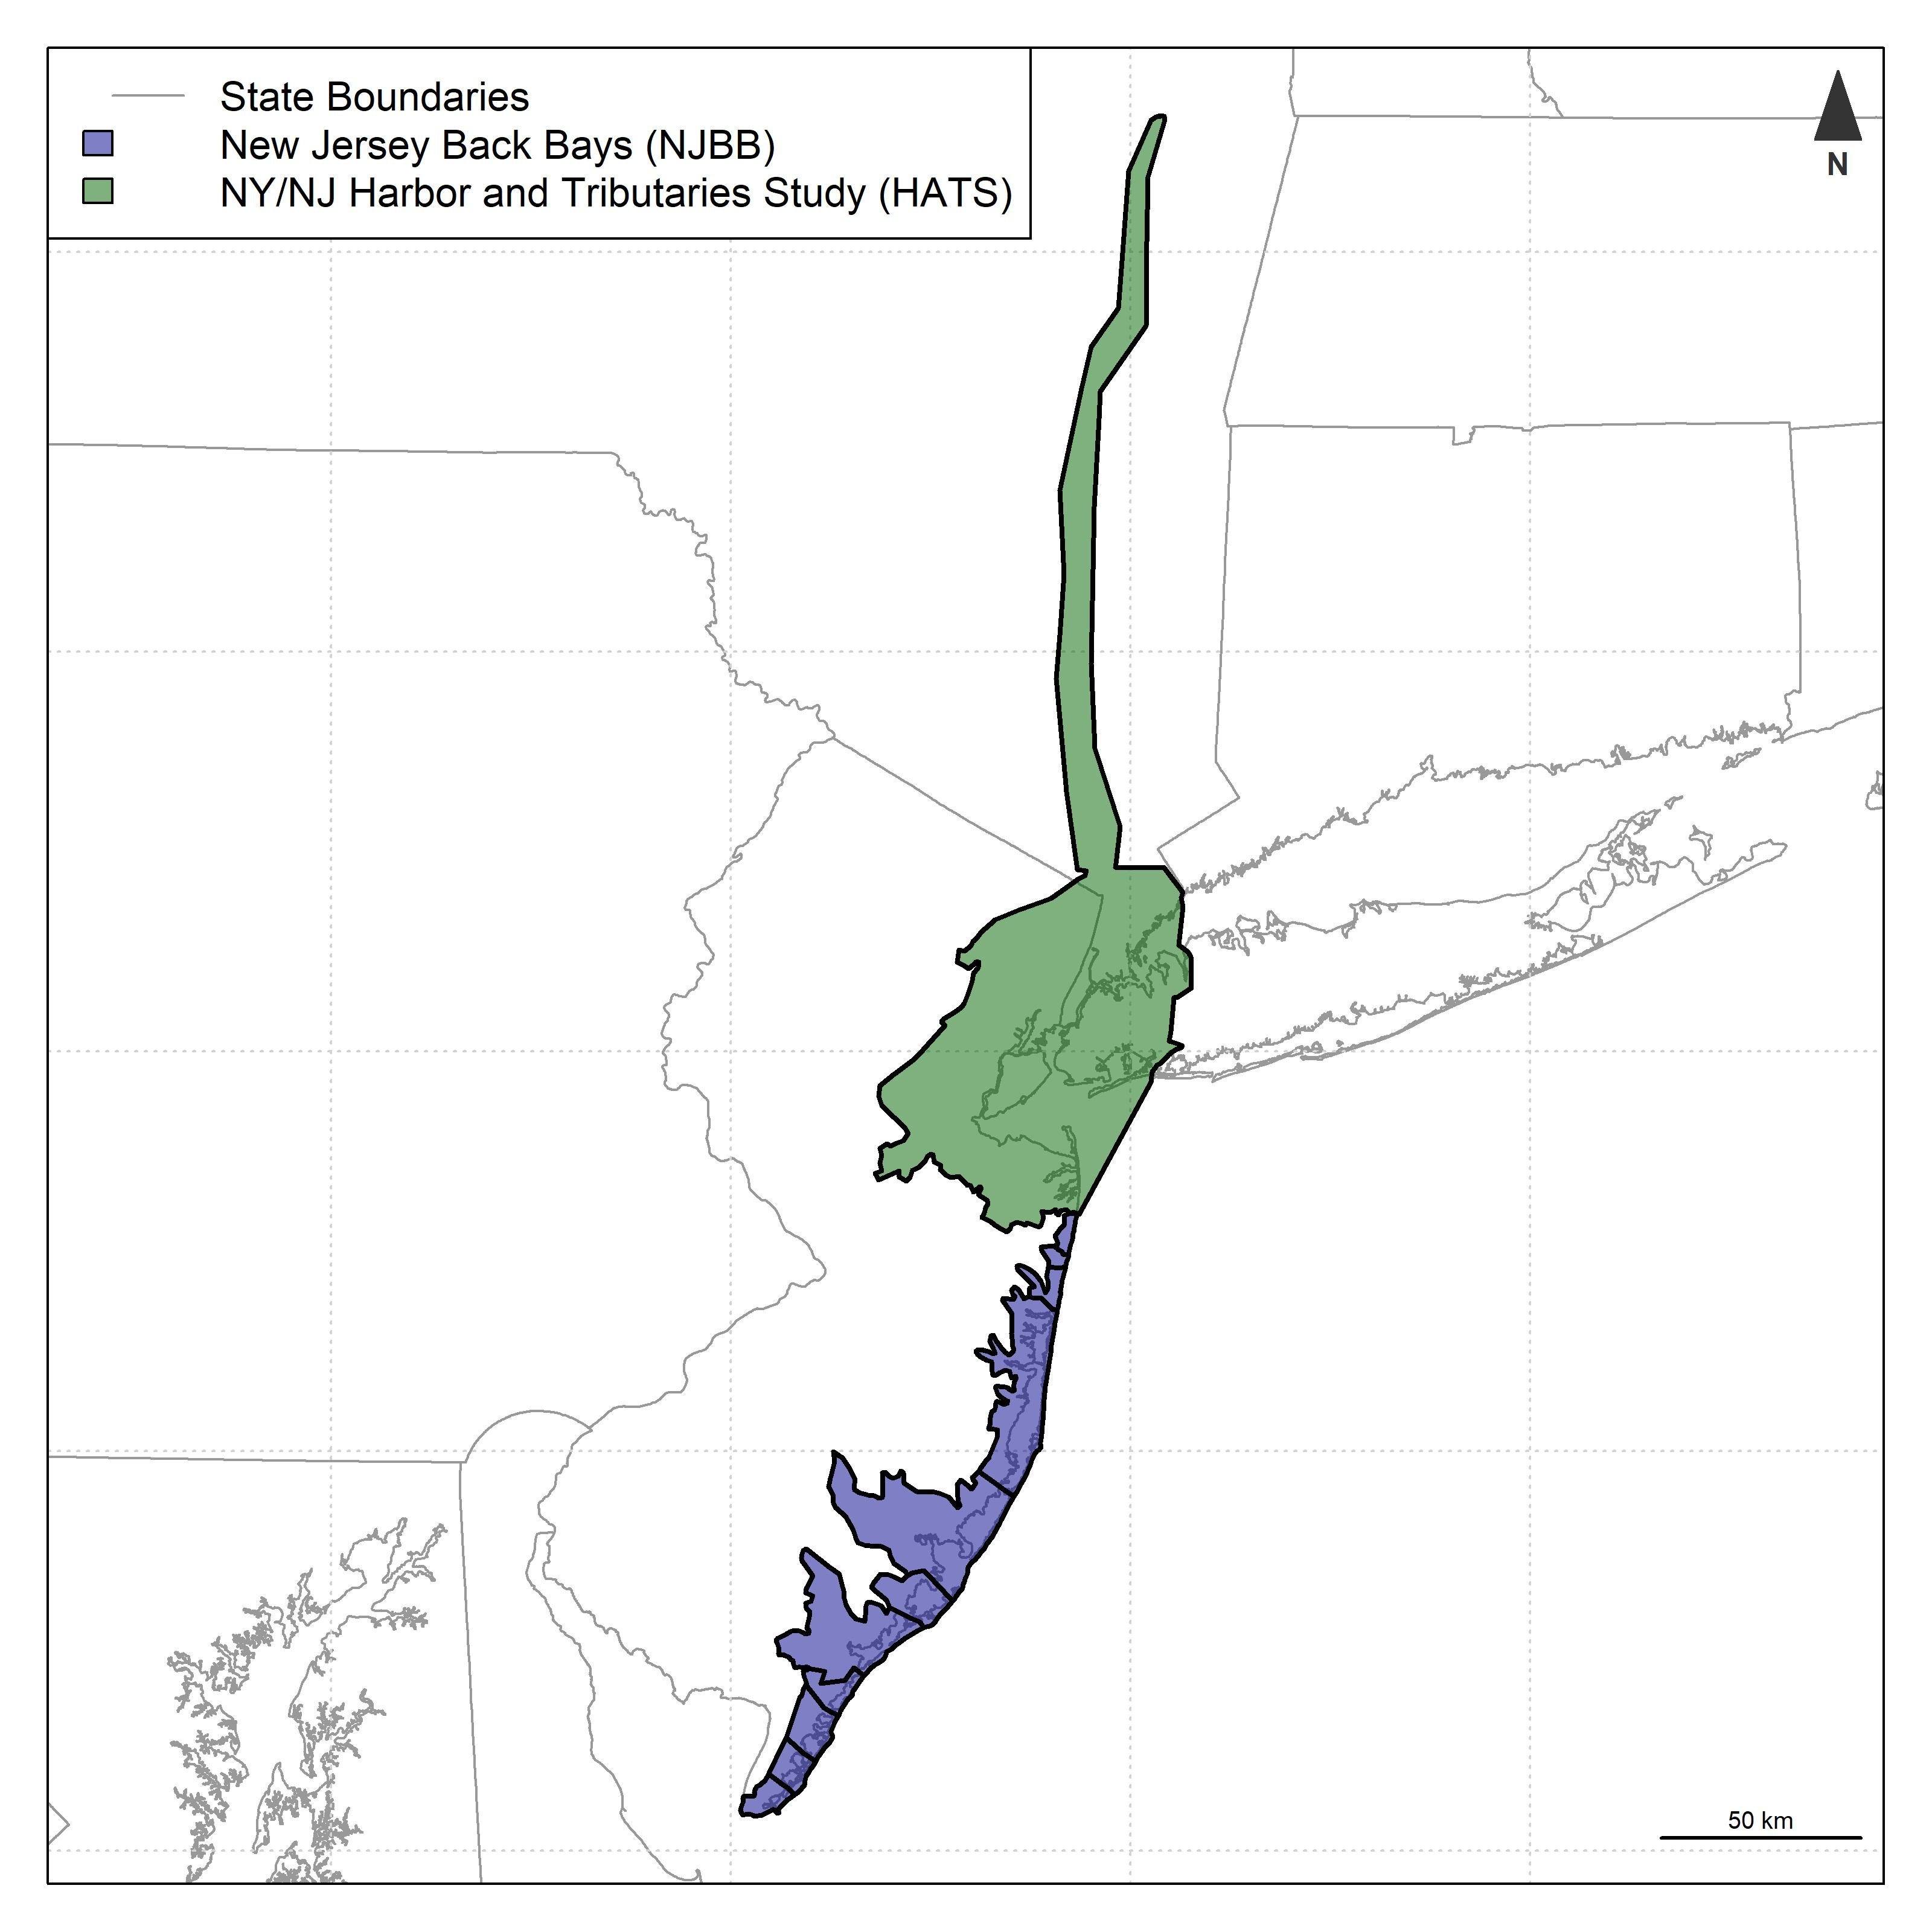
\includegraphics[width=44.44in]{ZZ_Fig01.01_USACE.Studies} \caption{USACE regional coastal storm risk management studies. NJBB and HATS are the primary focus of model development.}\label{fig:unnamed-chunk-2}
\end{figure}

In these study areas, the USACE is considering a diversity of measures for mitigating flood risks, including structural actions (e.g., levees, floodwalls, storm surge barriers), non-structural measures (e.g., buy-outs, elevation of structures, flood-proofing), and natural and nature-based features (NNBF, e.g., wetland creation, reefs for breakwaters). Environmental outcomes and acceptability are important constraints on plan selection, and recommended plans must be in compliance with environmental laws and regulations. Given the large spatial scope, these USACE studies are applying a ``tiered'' approach to compliance with the National Environmental Policy Act (NEPA). Tiered assessment intends to provide appropriate data at key planning milestones for complex studies with diverse environmental effects. In the context of these studies, a ``Tier 1'' Environmental Impact Statement (EIS) will be generated at the conclusion of the USACE Planning Process (i.e., in the Feasibility Report and Chief's Report). The ``Tier 1'' EIS is being developed with sequentially more accurate and precise information as the planning process proceeds through key milestones such as the Alternatives Milestone Meeting (AMM), Tentatively Selected Plan Milestone (TSP), and Agency Decision Milestone (ADM). A ``Tier 2'' EIS will be developed in Pre-Construction Engineering and Design (PED).

\hypertarget{problem-statement}{%
\section{Problem Statement}\label{problem-statement}}

The conceptual and numerical models presented here seek to articulate and quantify mechanisms of environmental impact of proposed coastal storm risk management alternatives. The following goals guided model development:

\begin{itemize}
\item
  Models should provide a general description of the \emph{relative} environmental effects of large-scale alternatives, which can inform the feasibility process and NEPA assessments.
\item
  Models must be able to forecast environmental effects over the project planning horizon (50-100 years) based on physical changes to ecosystems resulting from both background processes (e.g., sea level rise) and project alternatives (e.g., change in tidal regime from storm surge barriers).
\item
  Models should assess environmental effects by ecosystem type (e.g., marine deepwater vs.~estuarine intertidal) to inform mitigation actions.
\item
  Models should capture direct effects of actions at infrastructure locations (e.g., the footprint of a surge barrier) as well as indirect effects induced off-site from infrastructure (e.g., change in bay hydrodynamics associated with a storm surge barrier).
\item
  Models should be adaptable to new information and data as project planning proceeds.
\item
  Models should provide a consistent approach for environmental assessment, which can assist with communication of the cumulative effects of recommended alternatives across the region.
\end{itemize}

\hypertarget{report-overview}{%
\section{Report Overview}\label{report-overview}}

This report presents development and application of the New York Bight Ecological Model (NYBEM, ``nigh-bem''), which will ultimately consist of two separate but interlinked models. First, an index-based modeling framework (i.e., a habitat-suitability-style, quantity-quality approach) is developed her to assess patch-scale effects for six ecosystem types (e.g., estuarine intertidal zones). Second, a network-based model will be developed in the future to assess system-wide connectivity for migratory, aquatic organisms (e.g., anadramous fish). This report documents the technical details, use, and relevant information for USACE model certification (EC 1105-2-412, PB 2013-02) for the patch-scale, habitat-suitability model. The following sections summarize the major elements of model development:

\begin{itemize}
\item
  \emph{Model Development Process}: Summarizes the general scope of the model and approach for development.
\item
  \emph{Conceptualization}: Describes the overarching view of the structure and function of ecosystems in the New York Bight.
\item
  \emph{Quantification}: Reviews the technical details and numerical code of the six ecosystem-specific, patch-scale models.
\item
  \emph{Evaluation}: Assesses the model relative to underlying numerical accuracy, scientific theory, and usability.
\item
  \emph{Application and Communication}: Describes an application of the NYBEM to assess the existing condition in the New Jersey Back Bays.
\end{itemize}

\hypertarget{model-development-process}{%
\chapter{Model Development Process}\label{model-development-process}}

When used in the context of complex management decisions with many partners, environmental and ecological modeling often benefit from approaches that emphasize transparency, increase user input during development, and clearly communicate model assumptions and limitations \citep{van_den_belt_mediated_2004, voinov_modelling_2010, herman_unpacking_2019}. Here, a general five-step modeling process is followed that applies best practices in ecological model development \citep{grant_ecological_2008}. First, general relationships among essential ecosystem components are formally \emph{conceptualized} to tell the story of ``how the system works'' \citep{fischenich_application_2008}. Second, the model is \emph{quantified} using a formal structure of functional relationships, algorithms, parameters, and numerical code. Third, models are \emph{evaluated} relative to underlying scientific theory, numerical accuracy, and usability, which often entails techniques such as code checking, testing, verification, and sensitivity analyses. Fourth, a model is \emph{applied} to a given management question, scenario, or assessment. Fifth, a strategy is developed and executed to \emph{communicate} model development and application to technical and non-technical audiences. This process has been applied numerous times to select, adapt, or develop ecological models for USACE and non-USACE studies \citep[e.g.,][]{mckay_aligning_2019, herman_unpacking_2019}, and the framework is intended to draw heavily from existing knowledge, data, and tools.

USACE policy \citep{us_army_corps_of_engineers_assuring_2011} defines a model as ``a representation of a system for a purpose,'' and thus specifying a modeling purpose and objective is often a foundational step in the modeling process. \textbf{Here, our modeling objective is to articulate the mechanisms and magnitude of environmental effects of proposed coastal storm risk management actions in the New York Bight Ecosystem.} However, this model (like all models) is being developed in a constrained environment with limited time and resources. Three key issues constrained and guided NYBEM development, each of which is addressed in subsequent sections:

\begin{itemize}
\item
  The model domain is limited to the spatial extent of the focal USACE studies.
\item
  Model development is phased to align with USACE project planning milestones.
\item
  Transparency in model development and input from stakeholders and partners were actively embraced to increase the adoption and acceptance of the tools, given the high-profile nature of the studies.
\end{itemize}

\hypertarget{spatial-extent}{%
\section{Spatial Extent}\label{spatial-extent}}

The cumulative project area of the ongoing CSRM studies exceeds 3,000 mi\textsuperscript{2} and covers multiple states. The spatial extent of model application was defined by a sequence of three sequentially smaller filters (Figure 2):

\begin{itemize}
\item
  \emph{New York Bight}: The USFWS defined the ecosystems of the New York Bight in 1997 as the ``open ocean region south of Long Island and east of New Jersey, known as the New York Bight proper'' and all associated upstream estuaries, waters, and lands. This large spatial domain covers 31,276 mi\textsuperscript{2} (10,206 mi\textsuperscript{2} upland watershed and 21,070 mi\textsuperscript{2} estuarine or marine). Specifically, the watershed is defined by ten 8-digit Hydrologic Unit Code (HUC) watersheds (02020006, 02020007, 02020008, 02030101, 02030103, 02030104, 02030105, 02030202, 02040301, and 02040302). The USFWS Bight definition includes all marine ecosystems offshore. However, given the nearshore scope of USACE's studies, seaward extent is limited to ecosystems above a 20m depth contour (i.e., the USFWS definition of ``nearshore''). This watershed boundary and seaward limit have a total area of 13,420 mi\textsuperscript{2}\citep{us_fish_and_wildlife_service_usfws_significant_1997}. However, given the nearshore scope of USACE's studies, seaward extent is limited to ecosystems above a 20m depth contour (i.e., the USFWS definition of ``nearshore'')\citep{us_fish_and_wildlife_service_usfws_significant_1997}.
\item
  \emph{Project Boundaries}: The Bight ecosystem includes many upland and coastal ecosystems beyond the project boundaries (e.g., Eastern Long Island). The USACE study boundaries provide a second filter on the spatial limits of the NYBEM. The New York Bight ecosystem contained within the project boundaries has an area of 2,930 mi\textsuperscript{2}.
\item
  \emph{Aquatic Ecosystems}: A key focus of the NYBEM is assessment of indirect effects of proposed actions. Currently, upland and shoreline ecosystems above mean higher high water (MHHW) are not included in the models. Impact assessments from these systems (e.g., dunes, scrub-shrub, riparian zones) are better understood from prior impact analyses. Additionally, these systems are likely to experience fewer indirect impacts, and methods are generally available for assessing direct impacts. Upland ecosystems are not explicitly removed from the spatial domain at this phase, but are removed below through the absence of any patch-scale models at elevations above MHHW and the absence of hydrodynamic data in uplands.
\end{itemize}

{REPLACE FIGURE}

\begin{figure}
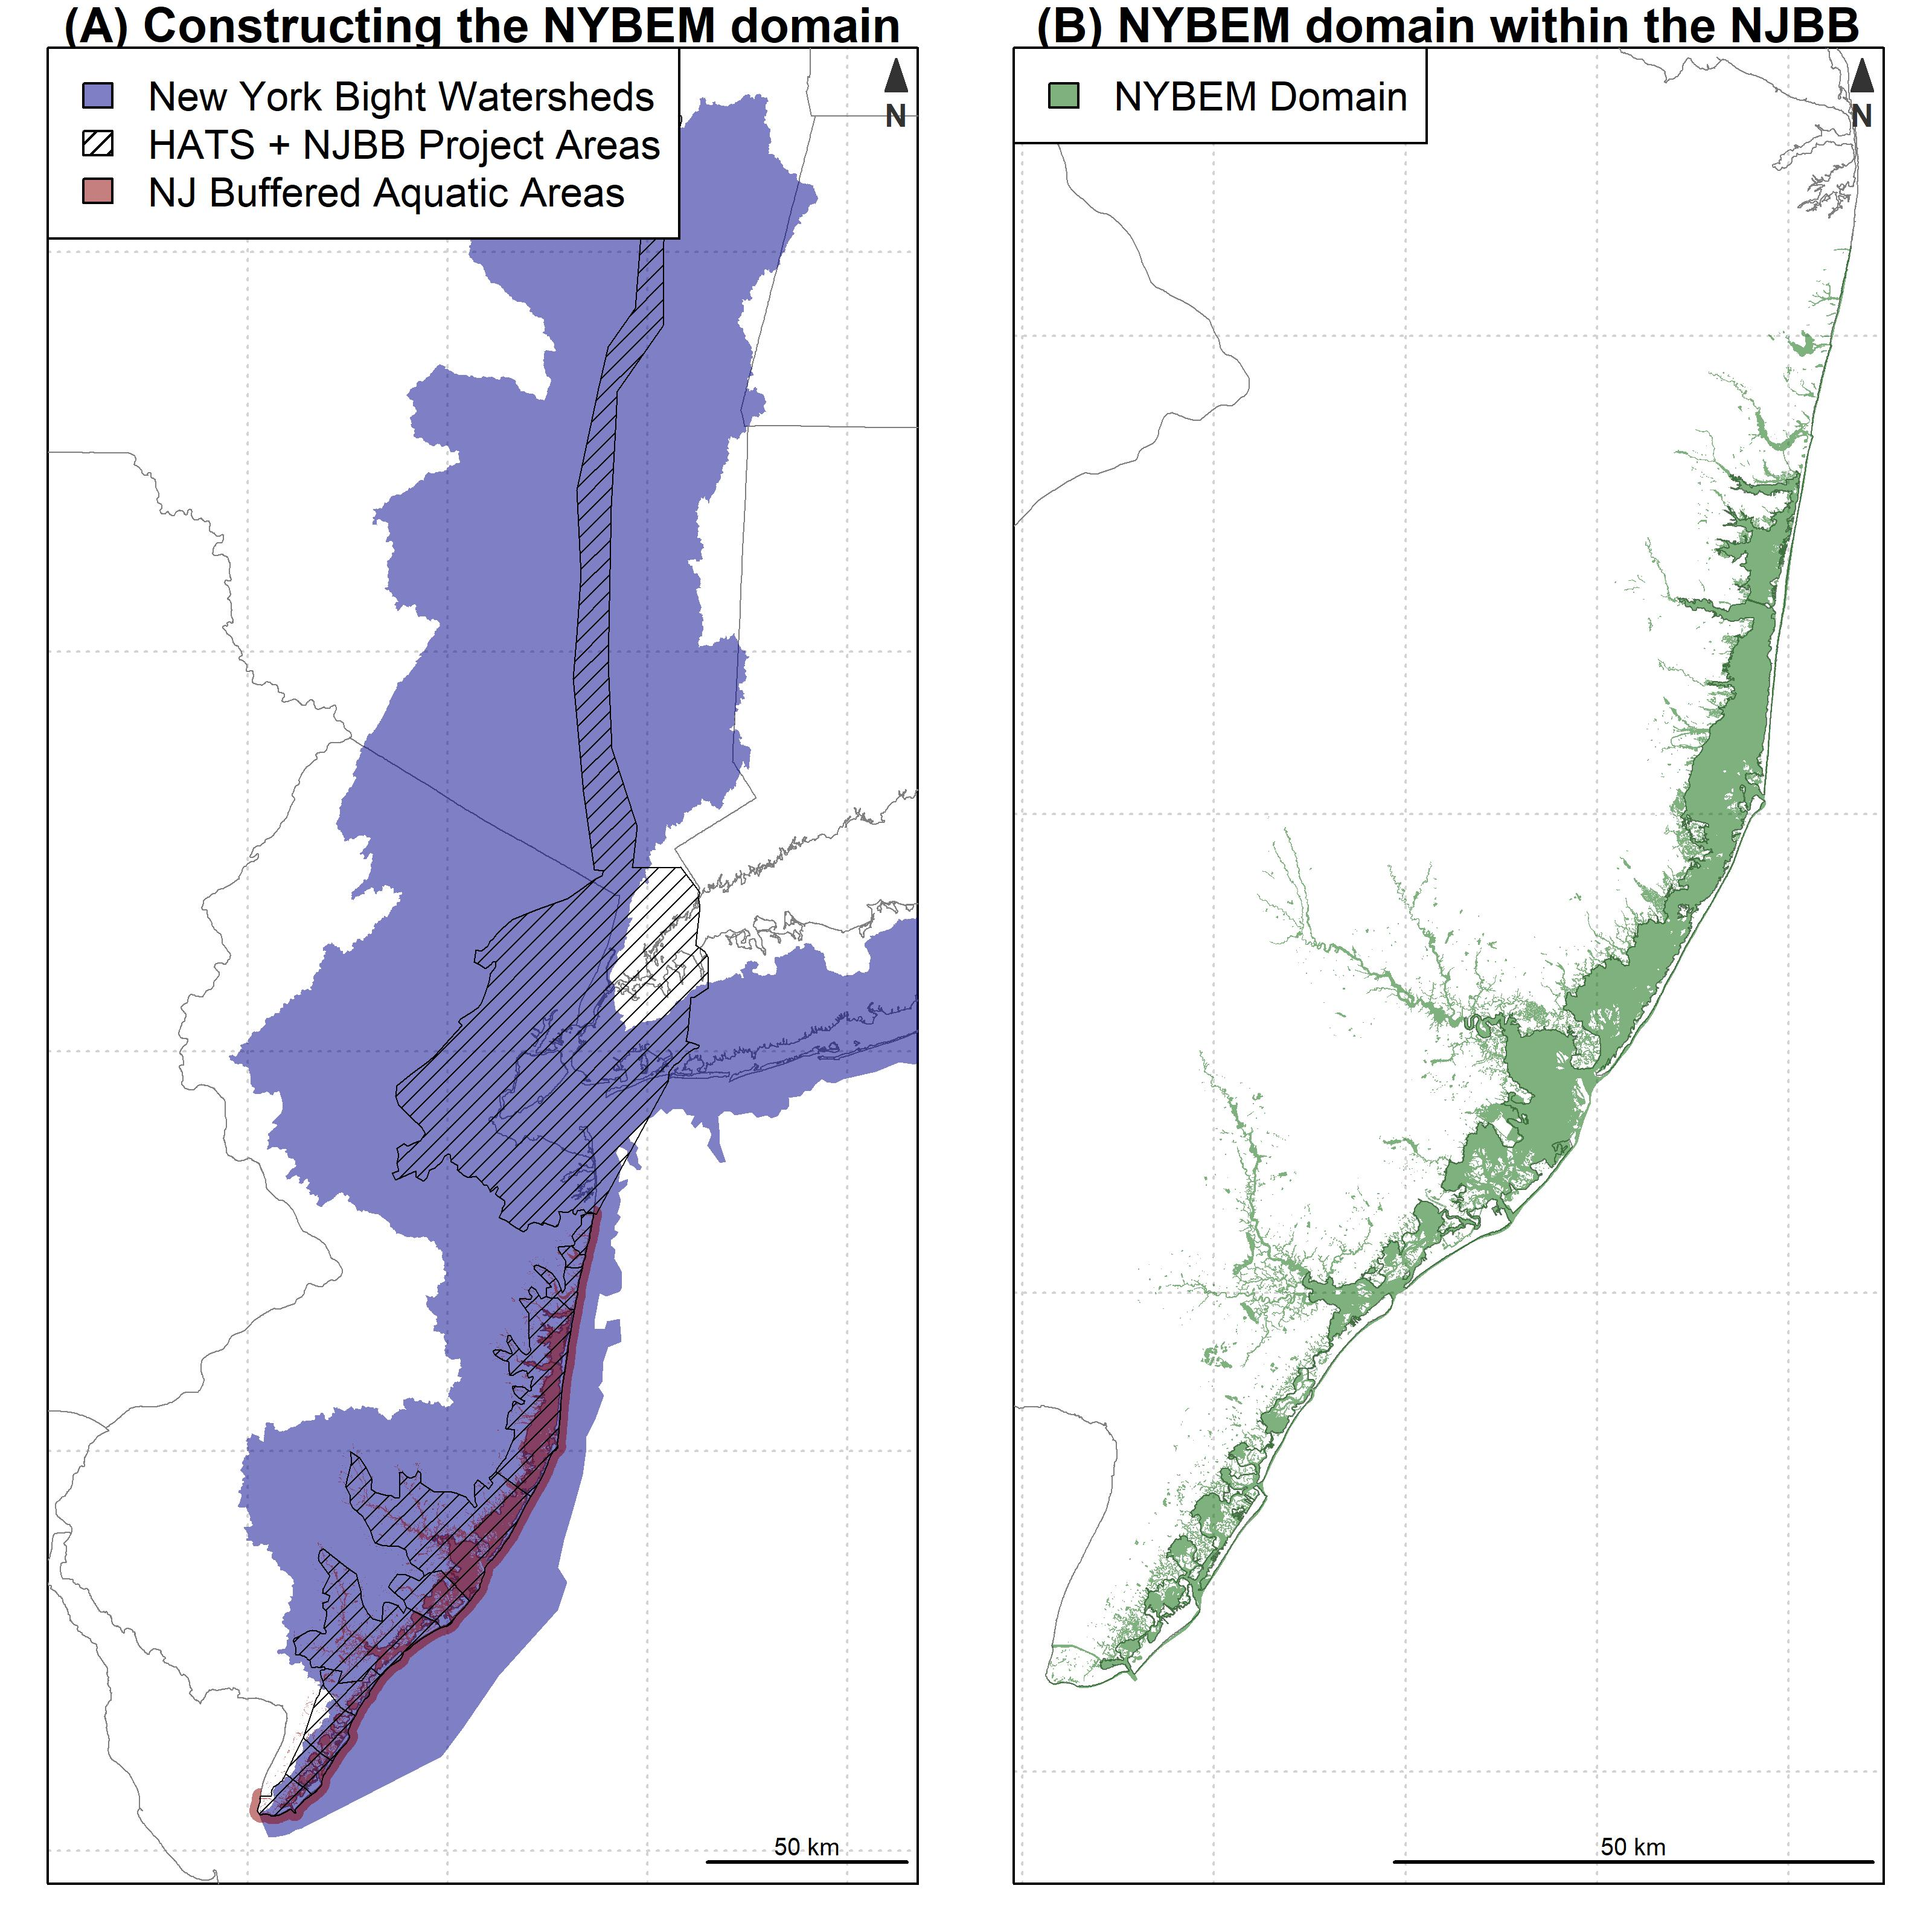
\includegraphics[width=44.44in]{ZZ_Fig02.01_NYBEM.Extent} \caption{NYBEM model domain: (left) Components of model domain, (right) NYBEM domain.}\label{fig:unnamed-chunk-3}
\end{figure}

\hypertarget{phased-approach}{%
\section{Phased Approach}\label{phased-approach}}

USACE planning studies sequentially make decisions about potential actions and buy-down risk and uncertainty to inform the next level of decision, before narrowing in on a recommended alternative. Furthermore, the USACE studies have proposed a ``tiered'' NEPA assessment, which is designed to gather more data and refine outcomes as a project proceeds. The NYBEM toolkit must be capable of responding to evolving project planning needs and data availability as these studies develop. As such, model development is explicitly being conducted in ``phases,'' and NYBEM tools and methods will evolve alongside project planning. In each phase, development will proceed iteratively through the cycle described above of conceptualization, quantification, evaluation, application, and communication. Table 2.1 presents key aspects of this phased approach to development.

\begin{table}

\caption{\label{tab:unnamed-chunk-4}Phased approach to development of the NYBEM.}
\centering
\begin{tabular}[t]{c|c|c|c}
\hline
District Planning Milestone & Interim Report & Draft Feasibility Report & Final Feasibility Report\\
\hline
Type of Decision & Preliminary Screening & Alternatives Analysis & Design and Operation of Recommended Alternative\\
\hline
Scope of Environmental Effects & Direct & Direct + Indirect & Direct + Indirect + Cumulative\\
\hline
Spatial Extent of Environmental Effects & Project footprint & Offsite hydrodynamic change & Mitigation requirements\\
\hline
Anticipated Outputs & Project footprint & Habitat Quantity and Quality (by type) & Habitat Quantity, Quality, and Connectivity (by type)\\
\hline
Analytical Effort & Rapid Screening & Moderate & Detailed\\
\hline
Hydraulic Forcing & Existing Condition & One year of tidal forcing + Two sea levels & Multiple years of tidal forcing + Multiple sea levels\\
\hline
Model Inputs & Footprint & Footprint + Tidal Range + Salinity + Hydrodynamics + Env Data & Footprint + Tidal Range + Salinity + Hydrodynamics + Env Data + Sediment + Temperature + Waves + Water Quality + Other\\
\hline
\end{tabular}
\end{table}

\hypertarget{mediated-modeling}{%
\section{Mediated Modeling}\label{mediated-modeling}}

The NYBEM intends to assess ecological consequences of alternative infrastructure options in a large, diverse ecosystem with many stakeholders and perspectives. ``Mediated modeling'' is used here to describe the family of techniques for building consensus among multiple partners to produce credible and defensible ecological models in a transparent way \citep{van_den_belt_mediated_2006}. There are many types of stakeholder-based model development processes that overlap in approach and emphasize collaboration: Model Prototyping, Participatory Modeling, Group Model Building, Companion Modeling and Mediated Model Development \citetext{\citealp[See reviews by][]{voinov_modelling_2010}; \citealp{gray_environmental_2017}; \citealp[and][]{hall_mediated_2019}}. These processes are generally well-suited to environmental management problems that are politically and publicly-sensitive, complex, and engage diverse audiences \citep{van_den_belt_mediated_2006}.

For NYBEM, a suite of workshop-based model development methods are adapted from \citet{herman_unpacking_2019}. These workshops utilize a lecture-exercise format, where participants are led through the theory of a particular aspect of modeling (e.g., conceptual modeling) and then apply said theory to a focal ecosystem (i.e., the New York Bight). The workshops structure the iterative development of NYBEM with subsequent research and synthesis between meetings (See McKay et al.~2021 for additional detail). Appendix B summarizes workshop logistics and focal topics. Key milestones in model development are briefly described below, but the overarching strategy is to engage larger audiences and more formal forms of model evaluation as the toolkit develops.

\begin{itemize}
\item
  \emph{Preliminary workshop with Philadelphia District} (January 2019): A preliminary conceptual model was developed with USACE Philadelphia District team members, which focused generally on issues potentially relevant for environment compliance at the broadest level.
\item
  \emph{USACE workshop with Philadelphia and New York Districts} (March 2019): A joint team from multiple USACE Districts was convened, and a strategy was proposed to develop NYBEM around key ecosystem types to reduce the dimensionality and complexity of the modeling problem and structure the path forward for model development.
\item
  \emph{Interagency conceptual modeling workshop} (June 2019): Fifty scientists and environmental managers (from federal, state, and local government as well as select non-profit organizations and academic units) were brought together to focus on the development of conceptual models supporting the NYBEM. This workshop utilized a series of posters and activities for attendees to provide input on relevant variables and processes for each ecosystem type.
\item
  \emph{Interagency numerical modeling workshop} (November 2019): A subset of attendees (20+) from the June 2019 workshop reconvened to discuss findings from the prior workshops. Prior to this meeting, the posters from June were formalized and synthesized with available scientific literature. At this meeting, attendees were able to review and revise preliminary versions of the model structure.
\item
  \emph{Phase-1 model documentation} (April 2022; this report): This report provides model development status as applied to the Draft Feasibility Report and Environmental Impact Statement for each study. USACE requires assessment and external evaluation of ecological models used in Feasibility-level planning decisions (i.e., model certification), and this report will be peer-reviewed according to these agency procedures.
\item
  \emph{Phase-2 development} (Fall 2022 / Winter 2023): Habitat quality and system connectivity tools will be further developed following the release of the Draft Feasibility Reports. Any modifications of models will also undergo review and certification.
\end{itemize}

Rapid timelines and iterative development encourage a transparent approach for model documentation as well. We adopt a growing family of methods for ``\href{https://ropensci.github.io/reproducibility-guide/sections/introduction/}{reproducible research},'' which embrace code and data sharing, enable review processes, and facilitate use of methods and results. Specifically, \href{https://rmarkdown.rstudio.com/}{R Markdown} is applied to development and document models, which are coded in the \href{https://cran.r-project.org/}{R Statistical Software}. These tools minimize data transfer errors and facilitate internal inspection of code as it is developed. Similarly, all model code is contained within a transportable R-package (i.e., \texttt{nybem}) following \href{https://r-pkgs.org/}{common development procedures}.

\hypertarget{conceptualization}{%
\chapter{Conceptualization}\label{conceptualization}}

The foundation of ecological modeling is a clear conceptualization of the ecosystem and an approach for translating the conceptual model into a numerical representation. This chapter describes an overarching conceptual model for the ecosystems of the New York Bight. A strategy is then presented for assessing these ecosystems relative to a habitat-style modeling approach, where the quantity and quality of each ecosystem type are computed separately and combined into an index of ecosystem integrity (i.e., a ``habitat unit'').

\hypertarget{conceptual-model}{%
\section{Conceptual Model}\label{conceptual-model}}

Conceptual ecological models are required for all USACE ecosystem restoration projects to increase understanding, identify potential alternatives, and facilitate team dialog \citep{fischenich_application_2008, us_army_corps_of_engineers_assuring_2011}. These same benefits apply for assessing environmental effects of proposed coastal storm risk management actions. Additionally, conceptual models also inform and structure the development of quantitative ecological models \citep{grant_ecological_2008, swannack_ecological_2012} such as the NYBEM. Conceptual models of the New York Bight were iteratively developed through the mediated workshops described in Section 2.3. Workshop ideas and content were synthesized with available literature, conceptual models of similar ecosystems (e.g., wetland function in Coastal Louisiana; \citet{twilley_formulation_nodate}), and existing regional conceptual models \citep[e.g.,][]{montagna_conceptual_2013}. A seven step conceptual model development process was interactively applied as workshops proceeded (Table 3.1).

\begin{table}

\caption{\label{tab:unnamed-chunk-5}Stepwise development of the overarching NYBEM conceptual model (following steps in Fischenich 2008).}
\centering
\begin{tabular}[t]{l|l}
\hline
Step & NYBEM Application\\
\hline
1. State the model objectives. & Our numerical modeling objective is to articulate the mechanisms and magnitude of environmental effects of proposed coastal storm risk management actions in the New York Bight Ecosystem. This conceptual model is intended to communicate the overarching scope of model development to a broad audience.\\
\hline
2. Bound the system of interest. & NYBEM is limited to the New York Bight Watershed with a seaward limit of a 20m depth contour. The models are further limited to aquatic ecosystems within the NJBB and HATS project areas. The NYBEM focuses only on effects to regional ecosystem, and other forms of environmental impacts (e.g., air quality, historic preservation) are addressed elsewhere in NEPA documentation.\\
\hline
3. Identify critical model components within the system. & This overarching conceptual model focuses on key ecosystem types and system-wide connectivity. Patch-scale models are defined from a combined classification based on @cowardin\_classification\_1979, USFWS (1997), and @montagna\_conceptual\_2013. A series of workshops and literature search were then used to identify ecosystem-specific model components associated with habitat quality (Chapter 4).\\
\hline
4. Articulate relationships among model components. & Only ecosystem types are presented, given the communication-driven purpose of this overarching model. More mechanistic conceptual models are presented for each ecosystem type in Chapter 4, which show connections between drivers and stressors, ecosystem states, and ecological outcomes.\\
\hline
5. Represent the conceptual model. & A simple graphic representation of the conceptual model (Figure 3.1) was developed to facilitate communication between project team members, sponsors, partner agencies, and other interested parties.\\
\hline
6. Describe the expected pattern of behavior. & The team qualitatively assessed the model along with potential gaps in ecosystem types and environmental impacts.\\
\hline
7. Test, review, and revise. & This overarching conceptual model was developed, presented, and refined based on a series of modeling workshops over a three year timeframe.\\
\hline
\end{tabular}
\end{table}

Ultimately, multiple conceptual models were developed for the New York Bight with different purposes. We first developed an overarching conceptual model communicating how a mosaic of regional ecosystems function together at a system-scale, which is intended for broad use within both technical and non-technical audiences (Figure 3.1). Three overarching systems were identified to frame model development: (1) nearshore / marine ecosystems, (2) estuarine ecosystems, and (3) system connectivity between multiple ecosystem types. These systems were distinguished based on differences in ecosystem processes such as wave energy and salinity dynamics, likely effects of proposed management alternatives, and potential differences in modeling philosophy (e.g., habitat models for nearshore and estuarine systems and a network approach to connectivity). Cumulatively, these three categories provide a means of assessing nearshore and estuarine ecosystems at a patch-scale as well as a means of assessing system-scale outcomes associated with connectivity. The ecosystem types were adopted from a combination of two existing classifications: \citep{cowardin_classification_1979, us_fish_and_wildlife_service_usfws_significant_1997}. In addition to this overarching model, mechanistic conceptual models were developed for each ecosystem type to guide quantitative model development (see Chapter 4), which are intended for technical audiences focused on the scientific details of ecological assessments.

\begin{figure}
\includegraphics[width=86.24in]{ZZ_Fig03.01_NYBEM.ConModel} \caption{Overarching conceptual model for the New York Bight.}\label{fig:unnamed-chunk-6}
\end{figure}

\hypertarget{major-ecosystem-types}{%
\section{Major Ecosystem Types}\label{major-ecosystem-types}}

Patch-scale assessments were developed for both the marine and estuarine ecosystems. Models were developed for each of the six major ecosystem types (Table 3.2). These ecosystems are defined from a combined classification based on \citet{cowardin_classification_1979} and \citet{us_fish_and_wildlife_service_usfws_significant_1997}. Salinity and tidal range differentiate these ecosystems, both of which can change under futures with and without management actions. While other analyses have developed ecosystem-scale assessments and models based on similar or more refined divisions in physical properties (e.g., \citet{clough_modeling_2016}, \citet{fischenich_application_2008}), the current criteria represent a compromise between the need for detailed assessment of the type and location of infrastructure impacts, and the need for a readily implementable rule set applicable at the broad spatial scale of the NYBEM.

\textbackslash begin\{table\}

\textbackslash caption\{\label{tab:unnamed-chunk-7}Definition of NYBEM ecosystem types. Cowardin et al.~(1979) define the marine-estuarine salinity transition based on a period of average annual low flow, which we define here as a 90\% exceedence probability (or 10th percentile salinity).\}
\centering

\begin{tabular}[t]{l|l|l|l}
\hline
Tidal Limits & Marine (Salinity >= 28psu) & Estuarine (Salinity = 0.5 to 28psu) & Freshwater (Salinity <= 0.5psu)\\
\hline
Deepwater (-2m to -20m) & Marine, Deep & Estuarine, Subtidal & Freshwater\\
\hline
Subtidal (MLLW to -2m) & Marine, Subtitdal & Estuarine, Subtidal & Freshwater\\
\hline
Intertidal (MHHW to MLLW) & Marine, Intertidal & Estuarine, Intertidal & Freshwater\\
\hline
\end{tabular}

\textbackslash end\{table\}

\hypertarget{habitat-style-modeling-philosophy}{%
\section{Habitat-Style Modeling Philosophy}\label{habitat-style-modeling-philosophy}}

Dozens of ecological modeling tools focus on coastal ecosystems. These models vary based on factors such as disciplinary perspective (e.g., hydrologic, geomorphic, ecological), the level of ecological hierarchy addressed (e.g., individuals, populations, communities, ecosystems), the basic approach to modeling (e.g., statistical, theoretical), input requirements (e.g., few parameters vs.~extensive geospatial layers), the treatment of time and space (e.g., lumped vs.~distributed), and the degree of development (e.g., long history vs.~ad hoc). However, multiple gaps in these tools are the driving motivation for developing the New York Bight Ecological Model (NYBEM).

\begin{itemize}
\item
  \emph{Comprehensive view of regional ecosystems}: Many existing ecological models focus on a subset of regional ecosystems (e.g., estuarine subtidal, but not marine subtidal) or focal taxa (e.g., fish, but not seagrass). The large spatial scope of the USACE study requires seamless landscape coverage of the study areas, as well as a consistent approach for assessing multiple ecosystem types simultaneously.
\item
  \emph{Connection to USACE management actions}: Existing tools often emphasize important physical forcings on ecosystems without a direct connection to USACE's proposed project action. For instance, a model may include marsh response to sea level rise, but be unable to incorporate marsh response to sea level rise in the presence of a storm surge barrier.
\item
  \emph{Indirect effects}: Models often emphasize direct changes at a site-scale rather than indirect effects of off-site changes. For instance, a model may assess habitat quality associated with substrate, but be unable to link to changes in substrate as a result of distant infrastructure effects (e.g., a storm surge barrier).
\item
  \emph{System-wide data}: Many valuable ecological tools have been developed at small spatial scales based on detailed site data (e.g., vegetation surveys or field assessment procedures). However, the extremely large scale of these projects precludes field data collection, and NYBEM inputs must be available for the entire model extent.
\item
  \emph{Rapid and phased application}: The USACE studies are assessing project outcomes within limited analytical timeframes. Therefore certain tools that might be applicable on longer time horizons (i.e., years) are not feasible in these short periods (i.e., months).
\end{itemize}

Given these challenges, the NYBEM seeks to build from the wide breadth of existing knowledge and models to develop a comprehensive set of tools that are directly applicable to the unique needs of planning USACE coastal storm risk management projects. The NYBEM draws from two distinct modeling approaches that are applicable at different scales. First, six patch-scale models are developed here, which use an index-based modeling philosophy assessing the quantity and quality of a given ecosystem type. Second, system-scale models will be developed in the future, which apply network-analytic methods to assess organismal connectivity. This report documents only the patch-scale models applicable in the six ecosystems shown in Table 3.2.

The NYBEM takes a common approach to ecological modeling based on quantity and quality of habitat. ``Index'' models \citep{swannack_ecological_2012} were originally developed for species-specific habitat applications (e.g., slider turtles), but the general approach has also been adapted to guilds (e.g., salmonids), communities (e.g., floodplain vegetation), and ecosystem processes (e.g., the Hydrogeomorphic Method). An index-based modeling approach is used for multiple reasons. First, index models directly respond to changes in physical properties and provide a clear link to changes in ecosystem quantity and quality resulting from future conditions with and without proposed actions. Second, index-based models align well with a phased model development approach. Third, index-based models are familiar to USACE decision-makers from diverse applications in other regions such as Louisiana coastal restoration (i.e., the Wetland Value Assessment), California bay restoration (i.e., East San Pedro Bay), and Gulf Coast harbor expansion (i.e., Mobile Bay). Notably, these examples each assess multiple habitat types (e.g., oyster, seagrass) and aggregate outcomes into an overall metric of ecological impacts or benefits.

In NYBEM, the quantity and quality of each ecosystem type are assessed separately. For instance, ecosystem extent and habitat quantity is rapidly delineated from modeled hydrodynamic conditions. Ecosystem quality is then assessed based on patch-specific data and known thresholds in ecological response (e.g., on a normalized 0 to 1 scale indicating ecological quality or function). The product of habitat quality and quantity provides a consistent metric across ecosystem types (i.e., ``habitat units''). Here, the terms ``habitat'' and ``ecosystem'' are used synonymously to indicate a given patch.

\hypertarget{quantification}{%
\chapter{Quantification}\label{quantification}}

The quantification phase of ecological model development formalizes a conceptual model in terms of mathematical relationships, model parameters, and a numerical algorithm \citep{grant_ecological_2008}. This chapter describes the NYBEM relative to model structure, associated numerical tools, and the theoretical underpinnings of the sub-models. In general, the overarching quantitative architecture of the NYBEM can be summarized in three major elements (Figure 4.1). First, model inputs are assembled in a geospatial database. Second, the model code is prepared as a ``package'' in the \href{https://cran.r-project.org/}{R Statistical Software}. Finally, the model outputs habitat quantity and quality as well as habitat units for each patch in the model domain.

\begin{figure}
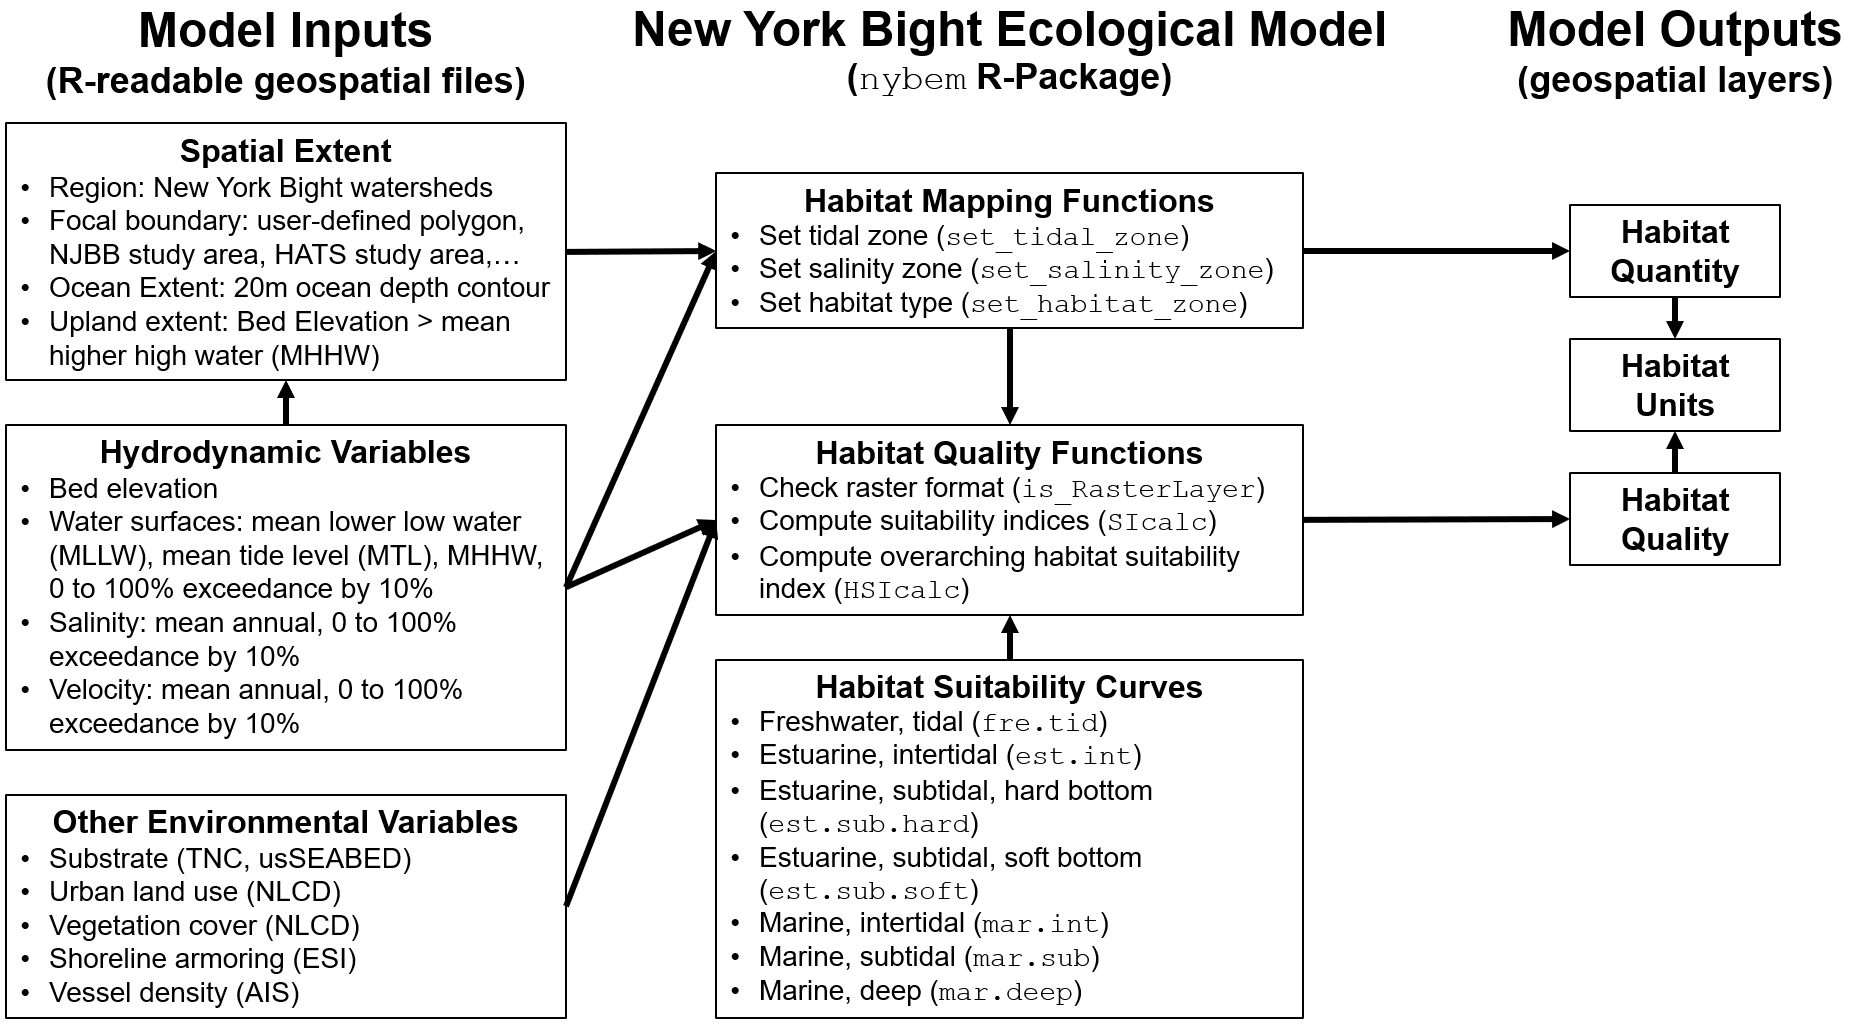
\includegraphics[width=17.47in]{ZZ_Fig04.01_NYBEM.Architecture} \caption{Quantitative architecture of the NYBEM.}\label{fig:unnamed-chunk-8}
\end{figure}

Input variables to NYBEM consist of three major groups of data layers. First, the spatial extent of a given model run must be defined. The NYBEM is constrained to applications within the region of the New York Bight watersheds (Section 2.1). Within that region, a focal area for the simulation must be specified, which can consist of a particular project boundary (e.g., NJBB or HATS) or a user-specified domain (e.g., a particular back bay). Within that focal area, the downstream and upstream extents of the model are specified based on the 20m ocean depth contour and Mean Higher High Water (MHHW), respectively. The second major group of variables consists of hydrodynamic inputs. These inputs may be computed for varying temporal windows (e.g., a month, a year, or a decade) depending on the project focus, and the inputs could be provided by a variety of hydrodynamic models or empirical data sources. Hydrodynamic variables characterize the bed elevation, water surface, salinity, and current velocity distributed throughout the project area. Third, a variety of environmental variables are compiled from national and regional data sets to inform habitat quality calculations.

All model code for the NYBEM is contained within an R-package (\texttt{nybem}, \href{https://github.com/MVR-GIS}{available via github}). Generally speaking, a package can be thought of as a fundamental unit of code that can include functions, data, documentation, and tests (\href{https://r-pkgs.org/}{Wickham and Bryan 2019}). Packages then provide a transportable and reproducible mechanism for code sharing and publication. The \texttt{nybem} package contains nine functions and associated testing trials. This chapter describes each function in detail, but they can be summarized briefly as:

\begin{itemize}
\item
  \texttt{nybem.domain}: This function defines the model domain based on the regional extent of the New York Bight watersheds, a user-specified focal area, a downstream extent of a 20m ocean depth contour, and an upstream extent based on bed elevations less than MHHW.
\item
  \texttt{patch.mapper}: This function maps the extent of NYBEM's six major ecosystem types (Table 3.2) based on user-specified data layers for bed elevation, MLLW, MTL, MHHW, and salinity.
\item
  \texttt{patch.rasterizer}: This function rasterizes the output of \texttt{patch.mapper} based on a specified grid resolution and aligns that layer with a specified spatial coordinate system.
\item
  \texttt{fre.tid}: This function computes habitat quality for any freshwater, tidal patches.
\item
  \texttt{est.int}: This function computes habitat quality for any estuarine, intertidal patches.
\item
  \texttt{est.sub}: This function computes habitat quality for any estuarine, subtidal patches.
\item
  \texttt{mar.int}: This function computes habitat quality for any marine, intertidal patches.
\item
  \texttt{mar.sub}: This function computes habitat quality for any marine, subtidal patches.
\item
  \texttt{mar.deep}: This function computes habitat quality for any marine, deepwater patches.
\end{itemize}

The first three functions can largely be thought of as fundamentally pre-processing the input data and mapping the extent of the six ecosystem types. For purposes of model development, these are relatively straight-forward and will be documented collectively. The latter six functions each compute a 0 to 1 metric of ecosystem condition (i.e., habitat quality) based on a unique set of input variables, equations, and parameters.

Each of these habitat quality sub-models followed a consistent set of development steps, which are documented throughout this chapter and briefly describe here. Preliminary variables were identified at a series of interagency workshops through a series of conceptual modeling exercises (Appendix A). Additional variables were added based on taxa-specific habitat suitability models (i.e., USFWS ``blue books''), relevant tools (e.g., New England Marsh Model), and literature reviews. A conceptual model was then developed for each ecosystem type to better understand how key variables relate and influence each other. An overarching list of regional and national data sets were also compiled to ensure that model variables could be assessed throughout the broad spatial extent of the New York Bight. Potential model variables were compiled along with the rationale for inclusion or exclusion. Finally, a numerical ``suitability index'' was developed for each variable remaining in the sub-model, which were based on existing suitability indices, published thresholds / responses, and professional judgment.

Ultimately, the \texttt{nybem} allows users to assess the extent and integrity of the six major ecosystem types represented in the NYBEM. The size and quality of a given habitat patch can provide useful metrics in their own right, or they may be summarized as an overarching ``habitat unit'' (i.e., the quantity of habitat in acres * patch quality assessed on a 0 to 1 scale).

\hypertarget{habitat-zonation}{%
\section{Habitat Zonation}\label{habitat-zonation}}

\texttt{patch.mapper}: This function maps the extent of NYBEM's six major ecosystem types (Table 3.2) based on user-specified data layers for bed elevation, MLLW, MTL, MHHW, and salinity.

In NYBEM, the quantity and quality of each ecosystem type may be assessed separately. For instance, ecosystems could be rapidly delineated from empirical data for the existing condition (e.g., field or tide gauge) or modeled hydrodynamic data for future conditions or proposed management actions. These delineated ecosystems can be summarized as an overarching habitat quantity in acres. Ecosystem quality may then be assessed based on patch-specific data and known thresholds in ecological response (e.g., on a normalized 0 to 1 scale indicating ecological quality or function). The product of habitat quality and quantity provides a consistent metric across ecosystem types (i.e., ``habitat units''). Here, the terms ``habitat'' and ``ecosystem'' are used synonymously to indicate a given patch.

The criteria for delineating ecosystems (Table 3) were subsequently programmed as a suite of logic statements for identifying the salinity zone, tidal zone, or ecosystem / habitat type for any given patch. The following functions input salinity, bed elevation, mean lower low water (MLLW), and mean higher high water (MHHW), and output a numerical code indicating salinity, tidal, and habitat zone as follows:

\begin{itemize}
\tightlist
\item
  \emph{Tidal Zone}: 1 = deep, 2 = subtidal, 3 = intertidal, and 4 = upland
\item
  \emph{Salinity Zone}: 1 = marine, 2 = estuarine, or 3 = freshwater\\
\item
  \emph{Habitat Zone / Ecosystem Type}: 1 = upland, 2 = marine, deepwater, 3 = marine, subtidal, 4 = marine, intertidal, 5 = estuarine subtidal, 6 = estuarine intertidal, or 7 = freshwater
\end{itemize}

\hypertarget{freshwater-tidal-zone}{%
\section{Freshwater, Tidal Zone}\label{freshwater-tidal-zone}}

Freshwater marshes are found in the topmost region of the estuary zone, from New York to North Carolina, where the entry of saltwater from tidal action is mitigated by a significantly higher amount of freshwater from upstream. These unique environments are ideally developed from sediments deposited by inflows from major freshwater rivers. Salt concentrations in tidal freshwater are typically less than 0.5 psu, although larger salinity pulses can occur during spring tides or periods of extremely low river discharge.

Tidal freshwater marshes provide significant nesting sites for a variety of species, including the marsh wren, and offer the primary habitat for emergent aquatic plants. Chronic sea-level rise is pushing the salt gradient upstream in rivers around the Atlantic Coast, causing vegetation to shift and some tidal freshwater marshes to become oligohaline wetlands. Many migratory (diadromous) fish species also rely on this habitat system, which is characterized by tidally impacted freshwater systems \citep{pasternack_biogeomorphology_2000}. Mussels, sturgeon, herring, and marsh wren are some of the species that live in this zone along with many micro-organisms.

The ability for the tidal freshwater ecosystem to support these various organisms can be modeled using salinity, vegetation coverage, episodic sediment deposition, and edge accretion parameters. Salinity concentration influences many chemical and physical ecological processes within the tidal freshwater ecosystem and supports euryhaline organisms. Emergent vegetation coverage provides habitat, mitigates inland flooding, and supports water quality within the tidal freshwater ecosystem. Water depth fluctuations support sediment deposition that bring an influx of organic nutrients into the ecosystem and mitigates sea-level rise. These quantifiable parameters all have influences on ecosystem services and habitat suitability within a tidal freshwater ecosystem.

Figure 4.2 presents a conceptual model of the freshwater, tidal ecosystem. This ecosystem is strongly influenced by effects on marsh elevations, salinity regimes, and the role of the system as a migratory corridor.

\begin{figure}
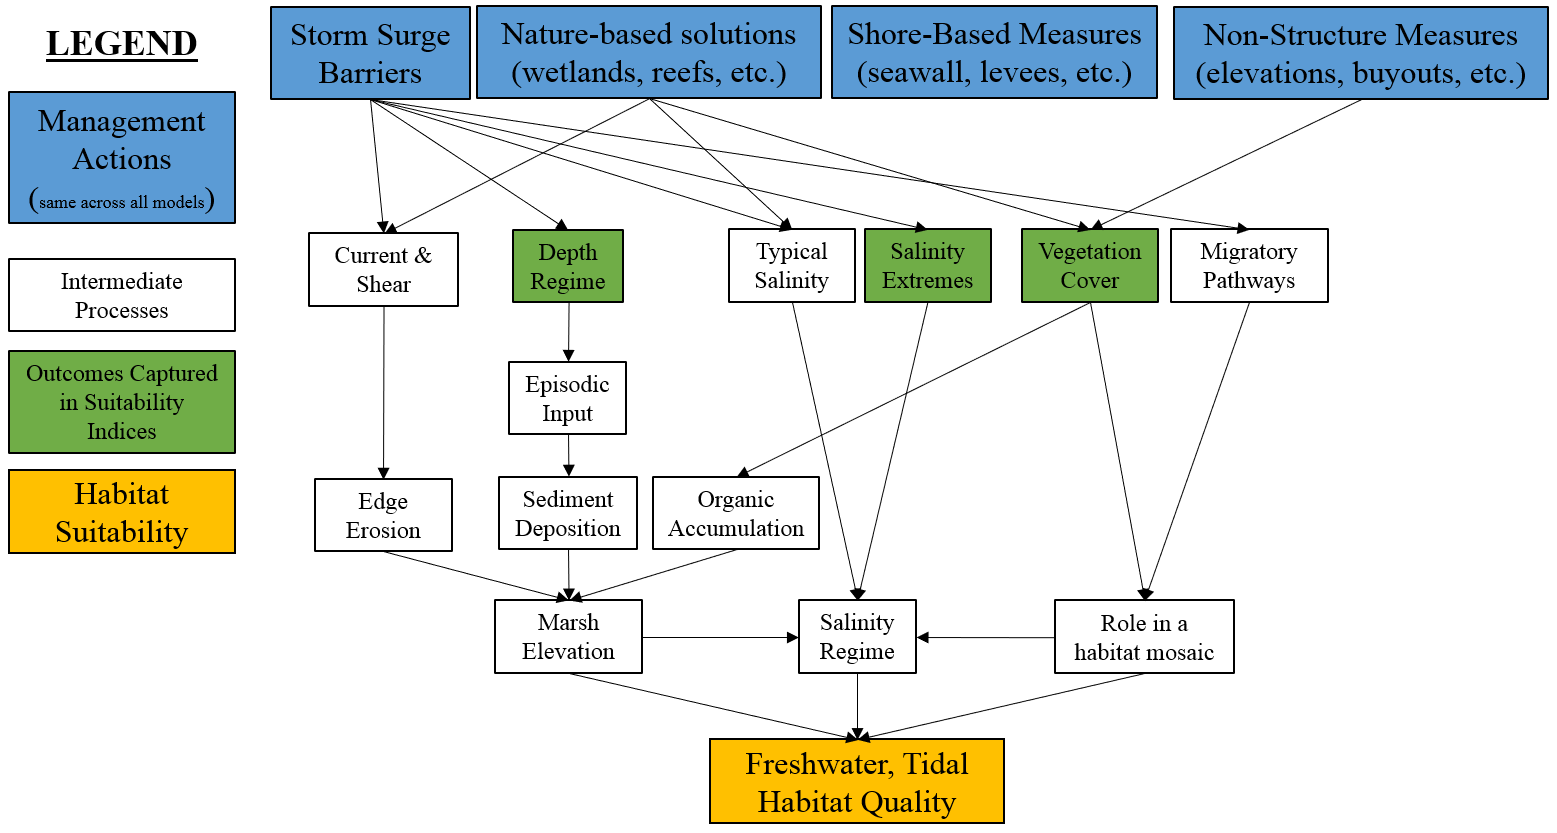
\includegraphics[width=21.58in]{ZZ_Fig04.02_Fresh.Tid_ConModel} \caption{Conceptual model for the freshwater, tidal submodel.}\label{fig:unnamed-chunk-9}
\end{figure}

The overall habitat suitability of the freshwater, tidal zone may then be aggregated into a single metric via an arithmetic mean of suitability indices for these four metrics.

\(I_{fresh.tid} = \frac{salinity + veg.cover + deposition + edge.change}{4}\)

Where \(I_{fresh.tid}\) is an overarching index of ecosystem quality for the freshwater, tidal zone, \(salinity\) is a suitability index relative to salinity, \(veg.cover\) is a suitability index relative to vegetative cover, \(deposition\) is a suitability index relative to episodic deposition of sediment, and \(edge.change\) is a suitability index relative to edge accretion. All indices are quality metrics scaled from 0 to 1, where 0 is unsuitable and 1 is ideal.

\begin{figure}
\centering
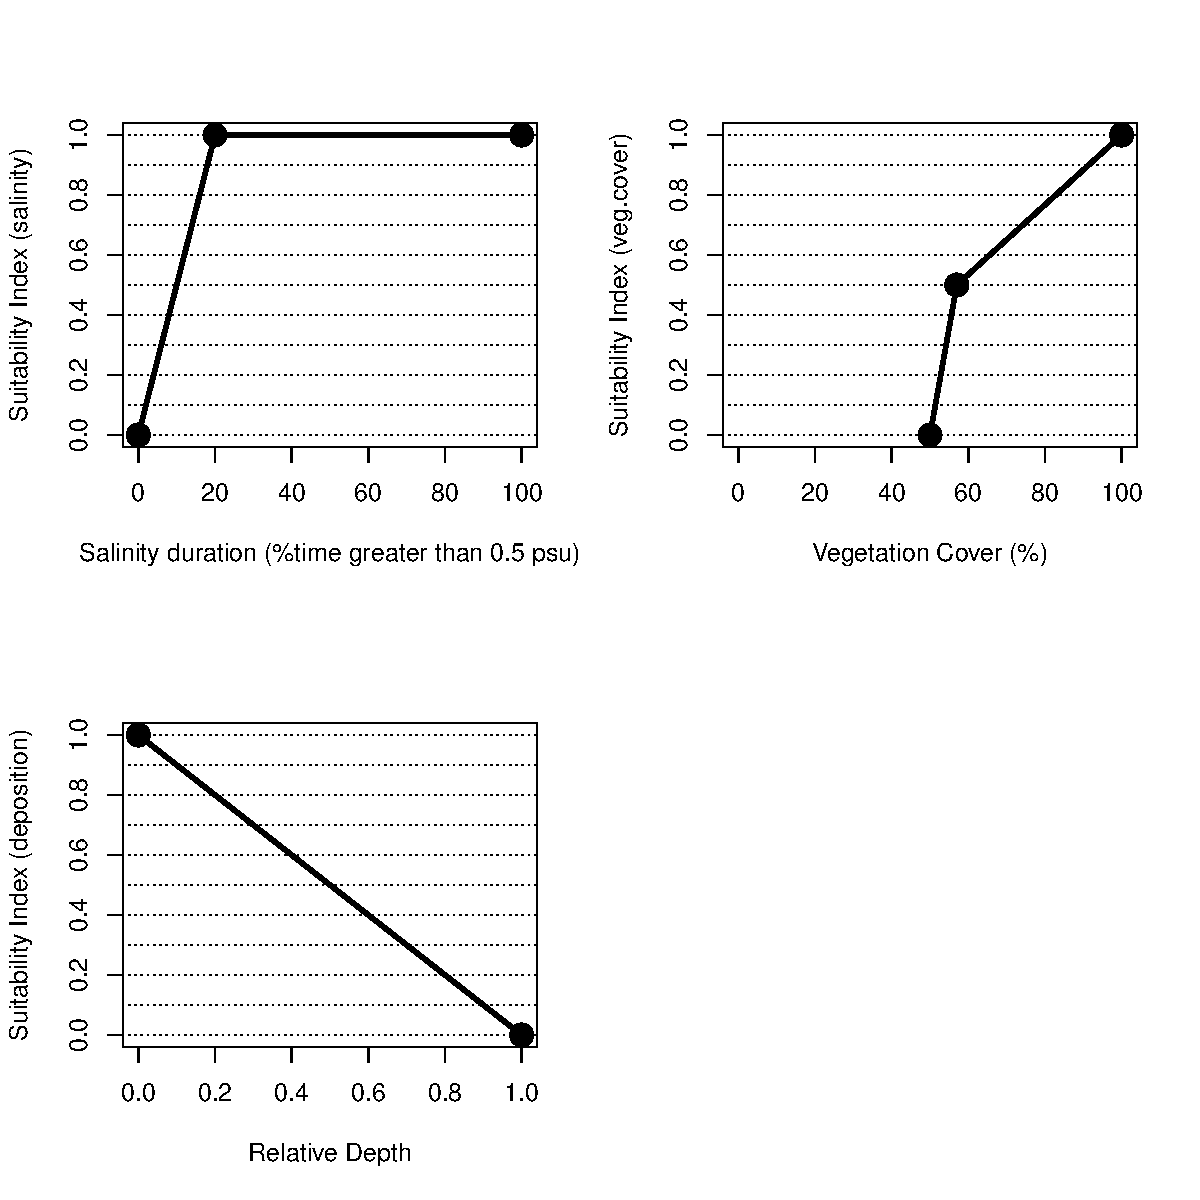
\includegraphics{_main_files/figure-latex/unnamed-chunk-10-1.pdf}
\caption{\label{fig:unnamed-chunk-10}Suitability index curves for the freshwater, tidal zone.}
\end{figure}

\hypertarget{salinity}{%
\subsection{Salinity}\label{salinity}}

Freshwater tidal wetlands are marshes and swamps with water that is less saline than brackish and is flooded on a regular lunar tidal basis. The salinity of the water varies from oligohaline to totally fresh (0 psu to 0.5 psu).

Salinity influences physical and chemical processes such as flocculation and the amount of dissolved oxygen (DO) in the water column, as well as the types of organisms that reside in a freshwater tidal ecosystem. Hurricanes and other storms may bring brackish water into the system, which is a significant natural disturbance. Because many plant species in these wetlands are not tolerant to brackish conditions, much of the vegetation is harmed as a result of these occurrences. For NYBEM, a proxy variable is used to account for these processes.

For NYBEM, the salinity regime is summarized through a metric of the percent of time salinity is less than the freshwater tidal ecosystem threshold of 0.5 psu. This approach assumes that saltwater inputs serve as disturbance on the ecosystem, and lower levels of salinity are preferred. Depth-averaged salinity is computed or measured at small time steps over and annual timeframe. These data may then be summarized as an ``exceedence curve'' with thresholds from 0-100\% in 10\% intervals. For NYBEM, this exceedence curve is used to calculate the percent of time salinity is less than or equal to 0.5 psu.

\emph{Please check equation}
This duration metric is then translated into a suitability metric as follows:

\[salinity.high.dur = \begin{pmatrix} 0.05*sal_{dur} & sal_{dur}=0-20\\
1.0 & sal_{dur}=20-100
\end{pmatrix}\]

Where \(salinity.high.dur\) is a suitability index relative to high salinity periods and \(sal_{dur}\) is the percent of time salinity is greater than the threshold for freshwater tidal habitat (i.e., salinity \textgreater{} 0.5 psu).

\hypertarget{vegetation-coverage}{%
\subsection{Vegetation Coverage}\label{vegetation-coverage}}

Freshwater Tidal Marshes are characterized by the dominance of herbaceous, shrubby, or emergent aquatic vegetation, with only a slight canopy of trees. Emergent vegetation coverage plays a crucial role in the tidal freshwater ecosystem. For avian taxa like the marsh wren, cover/reproduction appropriateness must be determined by the relative availability of emergent plants for nesting marsh wrens (Gutzwiller and Anderson 1987). Microorganisms frequently occupy headwaters marshes because they are contiguous with tidal creeks and contain an abundance of emergent vegetation \citep{rozas_rosubmerged_1988}.

Vegetation coverage within a freshwater marsh provides crucial habitat to a variety of unique animals and organisms. Vegetation within a tidal freshwater marsh is mainly brackish and cannot withstand long periods of increased salinity (over 0.5 ppt). Further, excessively moist or dry periods can cause additional stress to vegetation leaving the habitat susceptible to a salt intrusion event which can destroy vegetation and make the habitat totally unsuitable.

For the NYBEM tidal freshwater ecosystem submodel, vegetation coverage is quantified as the percentage of emergent aquatic vegetation. Emergent aquatic vegetation is a key habitat resource for species found within this ecosystem like marsh wren. Marsh wren are a key indicator species of ecosystem health because they are drawn to ideal wetland conditions. These important avian taxa are highly territorial and have a minimum habitat area of 50\% emergent vegetation coverage \citep{gutzwiller_habitat_1987}. Marsh wrens rarely breed in marshes with less than 57\% emergent vegetation \citep{gutzwiller_habitat_1987}. As a result, if there is less than this quantity of wetland habitat (emergent vegetation), the HSI is presumed to be 0. Vegetation coverage is a vital parameter of habitat suitability within a tidal freshwater ecosystem.

\[veg.cover = \begin{pmatrix} 0.0 & cover_{per}=0-50\\
0.0714*cover_{per}-3.57 & cover_{per}=50-57\\
0.0116*cover_{per}-0.16 & cover_{per}=57-100
\end{pmatrix}\]

Where \(veg.cover\) is a suitability index relative to vegetation coverage and \(cover_{per}\) is the percent of vegetation coverage.

\hypertarget{episodic-sediment-deposition}{%
\subsection{Episodic Sediment Deposition}\label{episodic-sediment-deposition}}

Tidal oscillations control the short-term dynamics of freshwater tidal wetlands, which feed nutrients into the environment and make them more fruitful and productive than most non-tidal wetlands (\citet{propato_evaluating_2018}). These tidal oscillations, as well as irregular weather events, deposit sediment and nutrients into the ecosystem.

Increased inundation in tidal freshwater marshes leads to more inorganic sediment deposition, which can assist tidal wetlands keep up with rising sea levels. As a result, marshes can migrate vertically to preserve their position in the tidal frame to some extent. In contrast, tidal freshwater ecosystems are frequently coupled with complicated geometry, such as a meandering channel with uneven depths and cross-sections. Because of the complicated geometry and huge fluctuations in freshwater discharge, there are strong seasonal variations in depth, which affect pollution transfer and algae development. When the depth of water within the ecosystem increases, the system is more susceptible to HABs, pollution, and habitat degradation. As a relative output of sediment, we adopt the ratio of water depth ranges to the tidal range, which we calculate as follows:

\emph{Please check equation}

\[d_{rel} = \frac{H_{max} - H_{min}}{Hmedian}\]
Where \(d_{rel}\) is water depth relative to the minimum and maximum water height measurements, \(H_{max}\) is the maximum depth observed over a hydrodynamic simulation period, \(H_{min}\) is the minimum depth observed over a hydrodynamic simulation period, and \(H_{median}\) is the median depth observed over a hydrodynamic stimulation period.

The relationship between sediment deposition and water level rise can be used to quantify habitat suitability within the freshwater tidal ecosystem. When water level increases, sediment deposition will be at an optimal level to support freshwater tidal habitat. This metric provides a relative accounting for the variances in depth across the ecosystem. For instance, \(d_{rel}>1\) occurs in portions of the freshwater tidal ecosystem that experience optimal sediment deposition conditions less than 90\% exceedance from \(H_{median}\), and in portions of the freshwater tidal ecosystem that experience optimal sediment deposition conditions less than 10\% exceedance from \(H_{median}\). In terms of habitat suitability, we assume that ideal values of this metric occur around 0.5 (near 1.1 meter depth) and suitability declines on either side of this threshold as follows:

\emph{Please check equation}

\[deposition = \begin{pmatrix} 0.02*d_{rel} & d_{rel}<0.5\\
-0.02*d_{rel}+2 & d_{rel}>0.5\\
0.0 & d_{rel}>1.0
\end{pmatrix}\]

Where \(deposition\) is a suitability index relative to episodic sediment deposition and \(depth_{m}\) is the change in depth in meters.

\hypertarget{potential-extension-of-freshwater-tidal-model}{%
\subsection{Potential extension of freshwater, tidal model}\label{potential-extension-of-freshwater-tidal-model}}

Edge Accretion: Edge accretion remains an important parameter of habitat suitability within the freshwater tidal ecosystem to include in the future development of the NYBEM. Freshwater tidal ecosystems have survived despite a rise in sea level, with tidal marsh heights remaining constant under freshwater circumstances, but future anticipated increases in relative sea-level rise might outpace marsh accretion rates, potentially resulting in the loss of these elevation-dependent coastal ecosystems (\citet{schile_modeling_2014}). Accretion is characterized as the accumulation of plant material, including roots and degraded material, from plants growing in the marsh, as well as growth via deposition of suspended particles during floods (allochthonous growth) (autochthonous growth)(\citet{schile_modeling_2014}).
In the SLAMM model, marsh erosion is exclusively modeled at the marsh-to-open-water interface, and erosion occurs only if fetch is sufficient. As a result, marshes have been proven to be less sensitive to this parameter than accretion parameters (MEM)(SLAMM)(\citet{morris_responses_2002};\citet{propato_evaluating_2018}). Edge Accretion can be quantified using parameters in marsh platform elevation, biomass increase, and tidal inundation, but face limitations from data availability and accessibility.

Depth zonation?

({ADD NOTES HERE.})

\hypertarget{estuarine-intertidal-zone}{%
\section{Estuarine, Intertidal Zone}\label{estuarine-intertidal-zone}}

Estuarine environments include marine water that has been diluted by freshwater runoff from the land \citep{prosser_impacts_2018}. Due to tidal influence, intertidal ecosystems are found between high and low tide, experiencing varying land and sea influences, whereas subtidal ecosystems are constantly submerged. The estuarine intertidal ecosystem considers areas with salinity values greater than 0.5 psu to 30 psu and elevation from MHHW to MLLW. Plant, animal, and microorganism populations, as well as their nonliving surroundings, interact as a working unit in intertidal ecosystems, which are exposed at low tides (Citation). Within the estuarine intertidal ecosystem, ecological processes are linked to physical and chemical characteristics. These characteristics can experience change under anthropogenic and climatic pressures that deviate from the homeostasis, or baseline, habitat condition. This can result in reduced habitat suitability across the estuarine intertidal ecosystem.

Tidal marshes are vegetated intertidal ecosystems found at the land-sea interface that serve as crucial transition zones for marine, freshwater, and terrestrial processes \citep{colombano_climate_2021}. Tidal marshes originated in a range of coastal and estuarine environments, and their location exposes them to a number of environmental factors (e.g., ocean currents, watershed hydrology) and environmental gradients (e.g., salinity)\citep{lauchlan_species_2020}. Broad-scale climatic changes are already affecting the timing, size, and duration of naturally varying environmental variables in estuarine, and freshwater settings. Understanding the changes in environmental stressors from climate change and sea level rise (SLR) on the tidal marsh ecosystem is critical to evaluate changes after the addition of storm surge barriers.

The following variables are accessible to the estuarine intertidal submodel portion of the NYBEM: salinity, episodic sediment deposition, edge erosion, vegetative cover, development of adjacent uplands, and the presence/absence of shoreline armoring.

\begin{figure}
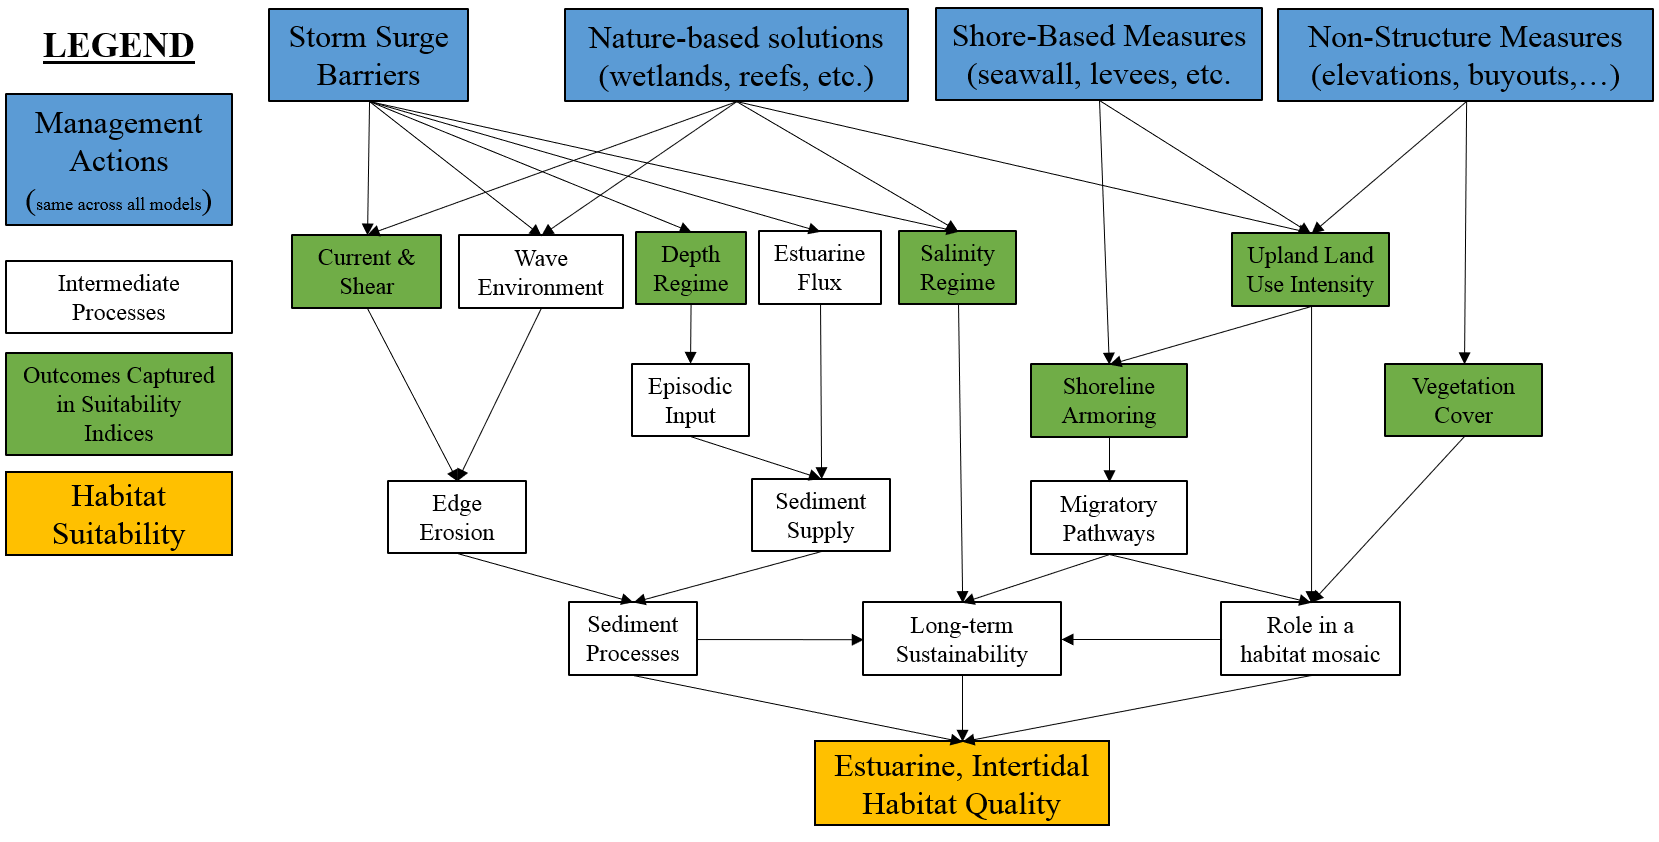
\includegraphics[width=23.04in]{ZZ_Fig04.04_Est.Int_ConModel} \caption{Conceptual model for the estuarine, intertidal submodel.}\label{fig:unnamed-chunk-12}
\end{figure}

The overall habitat suitability of the marine, intertidal zone may then be aggregated into a single metric via an arithmetic mean of suitability indices for these six metrics.

\(I_{est.int} = \frac{salinity + erosion + veg.cover + deposition + upland + shoreline}{6}\)

Where \(I_{est.int}\) is an overarching index of ecosystem quality for the marine intertidal zone, \(salinity\) is a suitability index relative to salinity, \(erosion\) is a suitability index relative to the edge erosion, \(veg.cover\) is a suitability index relative to vegetative cover, \(deposition\) is a suitability index relative to episodic sediment deposition, \(upland\) is a suitability index relative to adjacent upland land uses, and \(shoreline\) is a suitability index relative to shoreline armoring. All indices are quality metrics scaled from 0 to 1, where 0 is unsuitable and 1 is ideal.

\begin{figure}
\centering
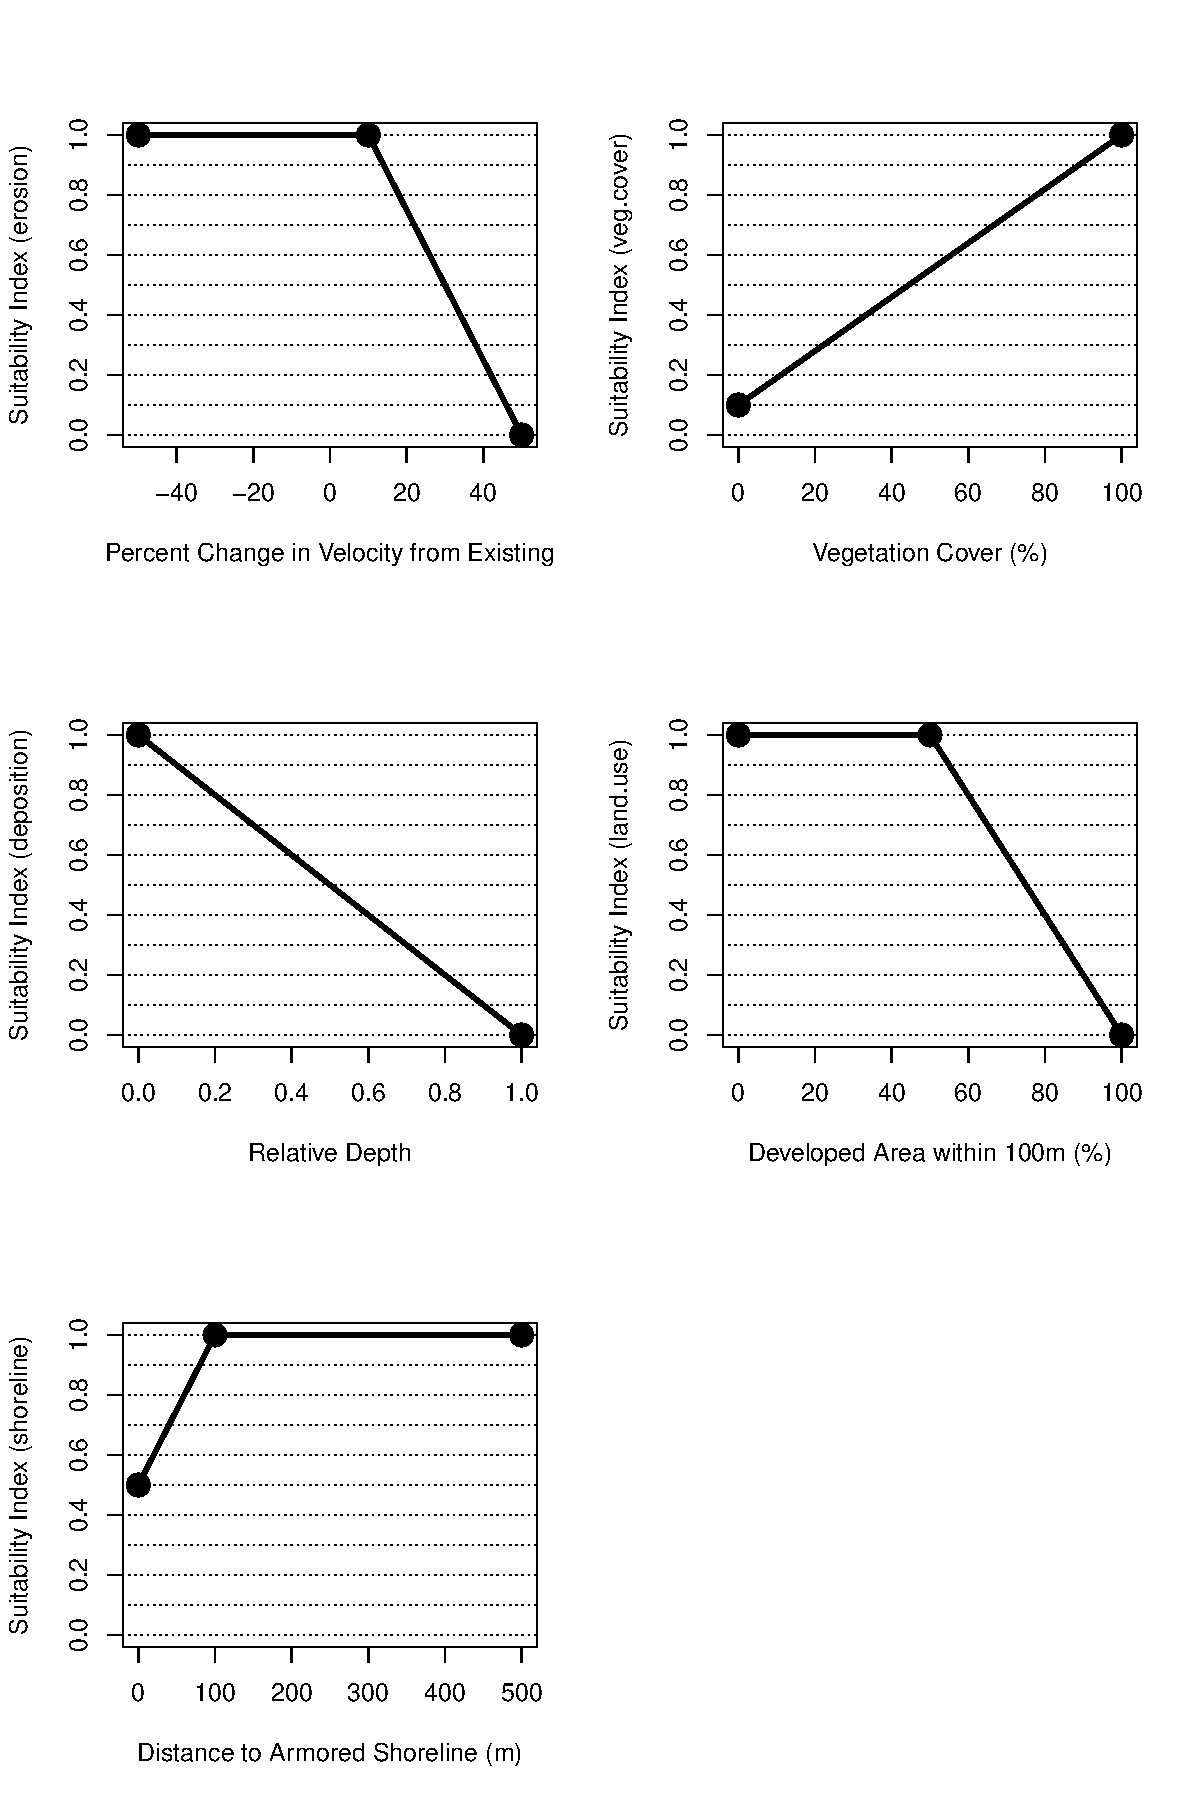
\includegraphics{_main_files/figure-latex/unnamed-chunk-13-1.pdf}
\caption{\label{fig:unnamed-chunk-13}Suitability index curves for the estuarine, intertidal zone.}
\end{figure}

\hypertarget{salinity-1}{%
\subsection{Salinity}\label{salinity-1}}

Salinity has an impact on physical and chemical processes including flocculation and the amount of dissolved oxygen (DO) in the water column, as well as the kinds of organisms that can live in an estuary. Estuarine organisms have evolved to cope with salinity fluctuations. Those that prefer fresher water at the upstream river end of the estuary to species that prefer saltier water at the downstream sea end usually form a gradient. Estuarine plants and animals suffer when extremely high salinities persist for lengthy periods of time. During instances of heavy freshwater inflows from rivers, harm might also occur. Extreme events are the issue in both scenarios.

Higher salinity, lower nutrient intake, and lower sediment inputs, that are associated with extremely low river inflow, can stress or kill plants and animals, limit productivity (owing to nutritional deficiency), and destroy marshes due to low sediment input. Low estuary salinity kills marine creatures when river inflow is extremely high; while excessive nutrient inputs contribute to algae blooms; and increased sediment input suffocates sea grasses and oysters \citep{hopkinson_lateral_2018}.

For NYBEM, the salinity regime is represented by a percentage of time where salinity is less than 30 psu, the estuarine intertidal ecological threshold. Freshwater inputs are assumed to be a disruption to the environment, and moderate salinity levels are recommended (less than 30 psu). Over an annual timescale, depth-averaged salinity is estimated or measured at short time steps. The data can then be summarized as a ``exceedence curve,'' with thresholds ranging from 0\% to 100\% in 10\% increments. The percent of time that salinity is less than or equal to 30 psu is calculated using this exceedence curve in NYBEM.

This duration metric is then translated into a suitability metric as follows:

\[salinity.mod.dur = \begin{pmatrix} -0.02*sal_{dur}+1 & sal_{dur}=0-50\\
0.0 & sal_{dur}=50-100
\end{pmatrix}\]

Where \(salinity.mod.dur\) is a suitability index relative to moderate salinity periods and \(sal_{dur}\) is the percent of time salinity is less than the threshold for marine habitat (i.e., salinity \textless{} 30 psu).

\hypertarget{edge-erosion}{%
\subsection{Edge Erosion}\label{edge-erosion}}

Climate change, pollution, and other anthropogenic effects are putting more pressure on terrestrial and marine ecosystems. Coastal flooding and shoreline erosion will likely become more common as sea levels rise and storm surges shift as a result of climate change. There is fear that tidal wetlands will drown as sea levels rise and sediment supplies to the shore decline across the world. Marsh sediment budgets are a geographically integrated measure of opposing constructive and destructive forces: a surplus of sediment can lead to vertical growth and/or lateral expansion, while a shortfall can lead to drowning and/or lateral contraction \citep{ganju_spatially_2017}. Many estuarine marshes face sediment deficits along the shoreline as a result of increased edge erosion. Edge degradation causes morphological changes that make it easier for waves to propagate to the marsh borders and promote the resuspension and export of sediments from the estuary \citep{li_wave-driven_2019}.

The percent change in edge erosion throughout the estuarine intertidal ecosystem is used to represent habitat suitability. When the percentage of shear stress for erosion is 10\% or greater, erosion occurs, resulting in a reduction in total marsh area and an increase in open water area. At a rate of 30\% shear stress from erosion, the habitat will no longer be suitable (habitat suitability equals zero.

\[erosion = \begin{pmatrix} 1.0 & vel_{delta}=-50-10\\
-0.025*urban_{per}+1.25 & vel_{delta}=10-50
\end{pmatrix}\]

Where \(erosion\) is a suitability index relative to edge erosion and \(vel_{delta}\) is the percent change in velocity relative to the existing condition.

\hypertarget{vegetation-cover}{%
\subsection{Vegetation Cover}\label{vegetation-cover}}

Vegetation provides various ecological services within the estuarine intertidal ecosystem, including providing a fish nursery environment, feed for migratory birds, nutrient cycling, carbon storage, and sediment stability. Therefore reductions of vegetative cover can have a significant impact on shallow marine ecosystems. Seagrass meadows are disappearing at an alarming rate in shallow coastal and estuary marine environments, with losses similar to tropical rainforests, mangroves, and coral reefs due to anthropogenic and climate stress \citep{walter_large-scale_2020}.

The loss of vegetative cover changes the dynamics near the seabed in locations where there was formerly vegetation. This loss transforms huge areas of the estuary from a deposition and accretion-friendly environment to one that favors suspension and erosion. For estuaries, high amounts of suspended particles and sediment-associated nutrients create a variety of environmental management issues \citep{cotton_effects_2006}.

For the NYBEM, habitat suitability increases as the percentage of vegetative cover increases throughout the habitat. When vegetative cover is equal to 100 percent, the estuarine intertidal ecosystem will have a high suitability value (greater than 90\%).

\[veg.cover = 0.9*cover_{per}+0.1\]

Where \(veg.cover\) is a suitability index relative to vegetation cover and \(cover_{per}\) is the percent of vegetation coverage.

\hypertarget{episodic-sediment-deposition-1}{%
\subsection{Episodic Sediment Deposition}\label{episodic-sediment-deposition-1}}

Estuaries are efficient sediment traps. Near-bottom circulation causes sediment flow convergence during the transition from brackish to fresh water, resulting in local maxima in suspended sediment concentration (SSC) and deposition rates. Marine materials are deposited from the continental shelf into estuarine habitats. Due to disparities in tidal currents (ebb versus flood tide), sediments are carried to supply sediment on varying time frames. In the estuarine intertidal ecosystem, sediment transport capacity is mostly determined by river discharge, by the timing of discharge events in relation to the spring--neap cycle, and subtidal oscillations in sea level \citep{prosser_impacts_2018}.

Due to the retreat of the salinity intrusion and increasing bed pressures, sediment deposition episodes can induce considerable bed resuspension in the estuary. Periodic flood and storm events are major drivers in sediment dynamics and contribute disproportionately to the total sediment discharge \citep{ralston_sediment_2013}. During these episodes of retreating salinity intrusions and increasing bed pressures, sediment deposition episodes can induce considerable bed resuspension in the estuary. The duration of high-discharge episodes in relation to the estuarine reaction time, a feature that fluctuates seasonally with discharge and estuarine length, also affects sediment transport capacity \citep{palinkas_sediment_2014}. These short-term events can cause changes in the local biological community and affect seabed stability and strength. As a relative output of sediment, we adopt the ratio of water depth ranges to the tidal range, which we calculate as follows:

\[d_{rel} = \frac{H_{max} - H_{min}}{Hmedian}\]

Where \(d_{rel}\) is water depth relative to the minimum and maximum water height measurements, \(H_{max}\) is the maximum depth observed over a hydrodynamic simulation period, \(H_{min}\) is the minimum depth observed over a hydrodynamic simulation period, and \(H_{median}\) is the median depth observed over a hydrodynamic stimulation period.

These then affect sediment mixing and activation, as well as tides, which affect water infiltration and exfiltration through the sediment \citep{nancy_jackson_armoring_2010}. During storms, erosion of the shoreline can result in the removal of material from the upper foreshore and deposition on the lower foreshore, or the foreshore moving horizontally landward. In coastal and estuary environments across the world, harmful algal blooms (HABs) have substantial economic, public health, and ecological consequences. The influx of additional nutrients following an episode of sediment deposition have been known to cause harmful algal blooms (HABs)\citep{ralston_temperature_2014}. Further, the frequent upturn of sediment can displace biological organisms. For example, horseshoe crabs are significantly affected by the above mentioned foreshore processes caused by episodic storms.

The relationship between sediment deposition and water level rise can be used to quantify habitat suitability within the esturarine intertidal ecosystem. When water level increases, sediment deposition will be at an optimal level to support esturarine intertidal habitat. This metric provides a relative accounting for the variances in depth across the ecosystem. For instance, \(d_{rel}>1\) occurs in portions of the esturarine intertidal ecosystem that experience optimal sediment deposition conditions less than 90\% exceedance from \(H_{median}\), and in portions of the esturarine intertidal ecosystem that experience optimal sediment deposition conditions less than 10\% exceedance from \(H_{median}\). In terms of habitat suitability, we assume that ideal values of this metric occur around 0.5 (near 1.1 meter depth) and suitability declines on either side of this threshold as follows:

\emph{Please check equation}

\[deposition = \begin{pmatrix} 0.02*d_{rel} & d_{rel}<0.5\\
-0.02*d_{rel}+2 & d_{rel}>0.5\\
0.0 & d_{rel}>1.0
\end{pmatrix}\]

Where \(deposition\) is a suitability index relative to episodic sediment deposition and \(depth_{m}\) is the change in depth in meters.

\hypertarget{developement-of-adjacent-upland}{%
\subsection{Developement of Adjacent Upland}\label{developement-of-adjacent-upland}}

The development of uplands within a watershed can have a direct and indirect impact on a variety of essential aspects in estuarine intertidal ecosystems. The combination of coastal erosion and upland development causes a ``coastal squeeze,'' in which low-lying, intertidal regions, that would usually recede inland in the face of sea-level rise, are diminished because man-made structures (e.g.~shoreline armoring) prevent such retreat \citep{prosser_impacts_2018}. This means that tidal marshes will need to shift upslope onto nearby uplands to survive during a period of rapid sea-level rise. Land management methods on the tidal marsh's upland border can help or hinder ecosystem migration in response to increasing sea levels \citep{anisfeld_upslope_2017}.

Both developed and undeveloped uplands can experience ecological stress as a result of climate change and land use changes (e.g.~addition of storm surge barriers, shoreline armoring). Climate change's effects on ocean and watershed systems are intertwined and set to interact.This is especially true in tidal marshes, which are biogenic environments that are sculpted by tidal and fluvial processes, and are dynamic and architecturally complex \citep{colombano_climate_2021}. Multiple stressors can affect the development of adjacent uplands such as low-flows, flooding, and reduced stream continuity \citep{talke_changing_2020}.

For the NYBEM, habitat suitability is modeled for an increase in development for adjacent uplands. When the percentage of developed adjacent uplands is greater than 10\%, habitat suitability in the estuarine intertidal ecosystem declines. When the development of adjacent upland reaches 100\% of the estuarine intertidal ecosystem, the habitat will no longer be considered suitable.

\[land.use = \begin{pmatrix} 1.0 & urban_{per}=0-50\\
-0.02*urban_{per}+2 & urban_{per}=50-100
\end{pmatrix}\]

Where \(land.use\) is a suitability index relative to adjacent upland land uses and \(urban_{per}\) is the percent of adjancent upland in developed (i.e., urban) land uses within 500m.

\hypertarget{shoreline-armoring}{%
\subsection{Shoreline Armoring}\label{shoreline-armoring}}

Natural biological processes and human-induced changes to the estuarine intertidal shoreline boundary are considered as components to a complex ecological system. The mean high-tide line is commonly used to determine shoreline boundaries and extent \citep{kittinger_shoreline_2010}. Shoreline modification called armoring has resulted in a considerable loss of coastal ecosystems from erosion, as well as a reduction in the resilience of these systems to disturbance \citep{kittinger_shoreline_2010}. Shoreline armoring involves placing hardened structures like bulkheads and revetments along the shoreline and as sea levels rise, these structures can prevent coastal marshes from spreading upland over time \citep{gardner_is_2021}.

Armoring is widespread throughout the United States, with extensive armoring found near urban areas \citep{morley_ecological_2012}. Shoreline armoring occupies 50-70\% of shorelines along urban coastal areas \citep{dugan_generalizing_2018}. Increasing shoreline development pressure and predicted sea-level rise suggest that the demand for shoreline armoring will continue to rise and expand throughout the future \citep{gardner_is_2021}. Shoreline armoring is correlated with decreased habitat complexity, and a reduction in connectivity to adjacent habitats \citep{morley_ecological_2012}.

The environmental consequences of armoring are context dependent, relying on characteristics of the environment and armoring structural factors \citep{dugan_generalizing_2018}. The type of structure placed (e.g., seawalls, bulkheads, revetments) and its relative placement on the coast profile will influence the biological reactions to armoring. Estuarine intertidal habitats that lack shoreline armoring have increased habitat suitability. For the NYBEM, the presence and absence of shoreline armoring will be utilized to derive information about the ability for multiple taxa to use the shoreline as migratory pathways.

\[shoreline = \begin{pmatrix} 0.05*dist_{armor}+0.5 & dist_{armor}=0-100m\\
1.0 & dist_{armor}>100m
\end{pmatrix}\]

Where \(shoreline\) is a suitability index relative to shoreline armoring and \(dist_{armor}\) is the distance to the nearest armored shoreline in meters.

\hypertarget{potential-extension-of-estuarine-intertidal-models}{%
\subsection{Potential extension of estuarine, intertidal models}\label{potential-extension-of-estuarine-intertidal-models}}

Describe model gaps here.

\hypertarget{estuarine-subtidal-zone}{%
\section{Estuarine, Subtidal Zone}\label{estuarine-subtidal-zone}}

This section presents development of the estuarine, subtidal submodel (est.sub). Estuarine subtidal habitat was defined as areas with elevations between MLLW and -20m with salinities ranging from 0.5 to 30 psu. In general, the est.sub seeks to capture the general condition and trajectory of the estuarine subtidal habitat using three different taxa (oysters, SAV, and clams) as indicators of ecosystem quality. Each taxa provides critical contributions to the overall quality of the ecosystem.

A conceptual model of the estuarine subtidal habitat was developed at a mediated modeling workshop (Appendix A). The conceptual model represented the major components affecting the quality of the ecosystem. Three main categories of drivers were identified: physical (water quality, velocity, sedimentation), anthropogenic (vessel traffic and development stress), and biological (SAV, benthic organisms, fish) with interactions among the categories. Conceptual models were then refined in two key ways (Figure XX). First, it was assumed that essential fish habitat would be present if oysters, SAV, and clams were present, so this variable was removed. Second, substrate type is a major driver of SAV, oysters, and clams. In general, the ecosystem can be coarsely divided into hard bottom and soft bottom habitats roughly correlated with oysters and SAV/clams, respectively. The unique characteristics and drivers of these habitats led to splitting the est.sub model into modules for each of these substrate types.

\begin{figure}
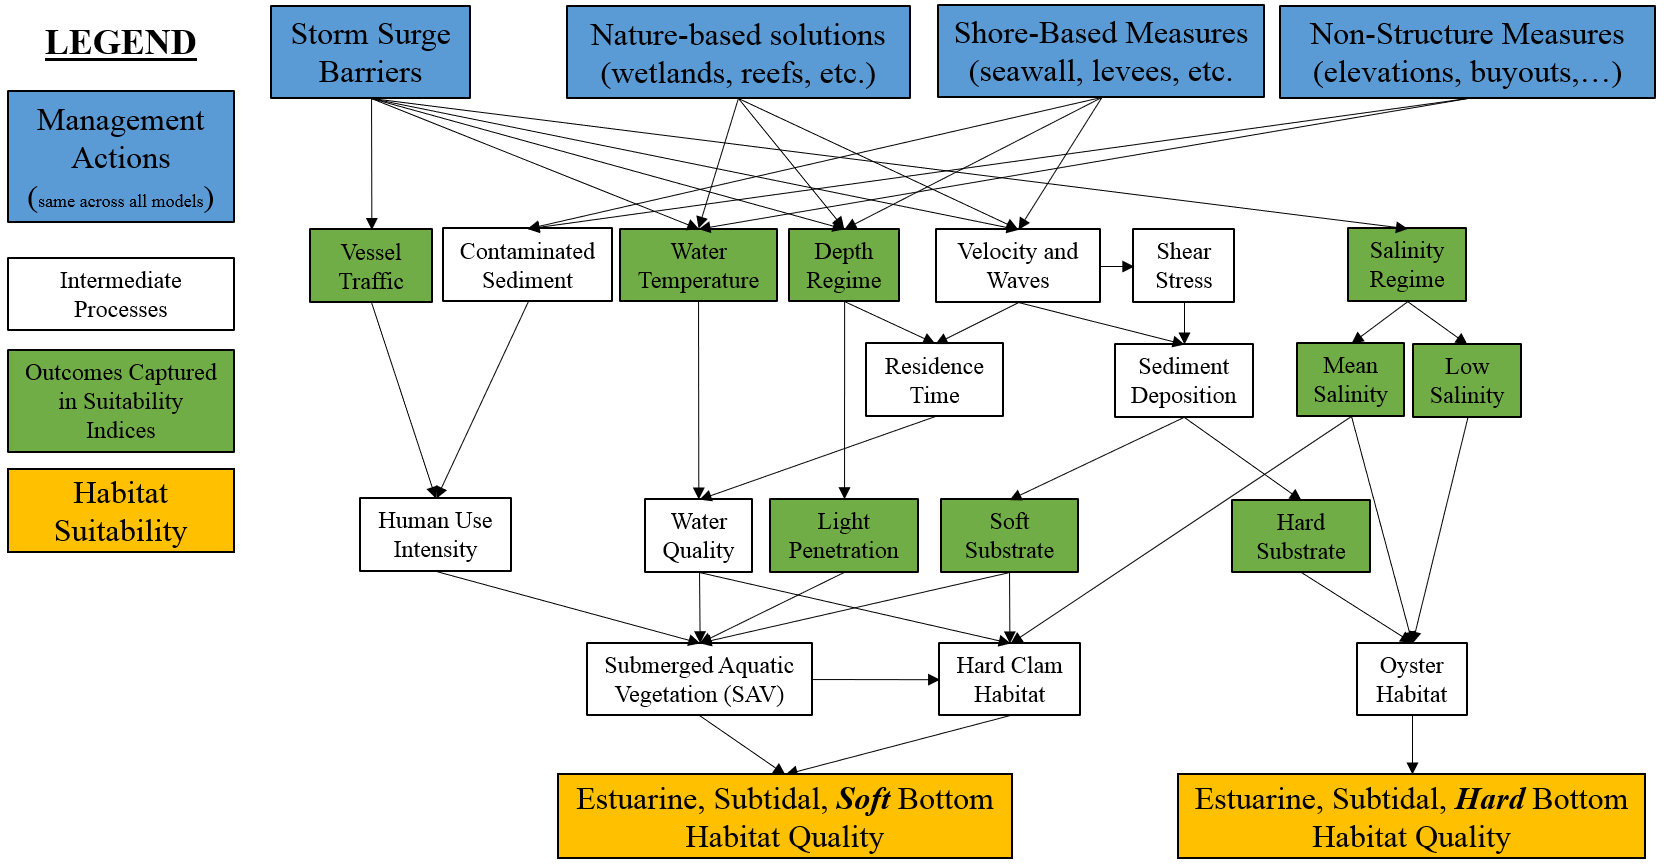
\includegraphics[width=23.11in]{ZZ_Fig04.06_Est.Sub_ConModel} \caption{Conceptual model for the estuarine, subtidal submodel.}\label{fig:unnamed-chunk-15}
\end{figure}

The est.sub modules was split into hard and soft bottom habitats (\texttt{est.sub.hard} and \texttt{est.sub.soft}, respectively). \textbf{Insert text differentiating hard bottom and soft bottom habitat}. All substrate data are merged from the \href{https://maps.coastalresilience.org/newjersey/\#}{TNC Substrate Map} and the \href{https://www.usgs.gov/programs/cmhrp/science/accessing-usseabed}{usSEABED}. Grain size are from XXX (\textbf{DO WE HAVE THIS?}), and fine substrate composition are from TNC.

est.sub.hard
Salinity = 0.5 to 30ppt
Subtidal (MLLW to -20m)
Median grain size \textgreater= coarse sand

est.sub.soft
Salinity = 0.5 to 30ppt
Subtidal (MLLW to -20m)
Median grain size \textless= coarse sand

Alternative approach\ldots known or historic hard bottom (i.e., any historic mapped oyster reef)?

\hypertarget{hard-bottom-habitats}{%
\subsection{Hard Bottom Habitats}\label{hard-bottom-habitats}}

Oysters are a major indicator of the integrity of hard bottom habitats in the New York Bight, and the hard bottom submodel is represented by an \textbf{adaptation} of the Oyster Habitat Suitability Index Model (OHSIM \citet{swannack_robust_2014}). The OHSIM is a USACE-certified model for the Eastern oyster (\emph{Crassostrea virginica}). OHSIM is a spatially-explicit, grid-based index model that uses a series of linear equations to calculate habitat suitability for \emph{C. virginica}. The model consists of four variables: substrate and three measures of salinity -- 1) mean salinity during spawning season, in which spawning and spat set have a higher optimal salinity than for survival of adults, 2) annual mean salinity, which is the expected range over which adult oysters are viable, and 3) minimum annual salinity, which defines the impacts of high mortality events resulting from lower salinities due to freshwater influxes \citep{soniat_understanding_2012}. Variables are briefly described below, and more details can be found in \citet{swannack_robust_2014} and EcoPCX documentation.

For the NYBEM, spawning season salinity data were not available, so only three variables are used. The overall habitat suitability of the estuarine, subtidal, hard bottom ecosystem is aggregated into a single metric via a geometric mean of these three suitability indices (following the OHSIM).

\(I_{est.sub.hard} = {(cultch * sal.min.ann * sal.mean.ann)}^{1/3}\)

Where \(I_{est.sub.hard}\) is an overarching index of ecosystem quality for the estuarine, subtidal, hard bottom habitats, \(cultch\) is a suitability index relative to hard bottom composition, \(sal.min.ann\) is a suitability index relative to minimum annual salinity, and \(sal.mean.ann\) is a suitability index relative to mean annual salinity. All indices are quality metrics scaled from 0 to 1, where 0 is unsuitable and 1 is ideal.

\begin{figure}
\centering
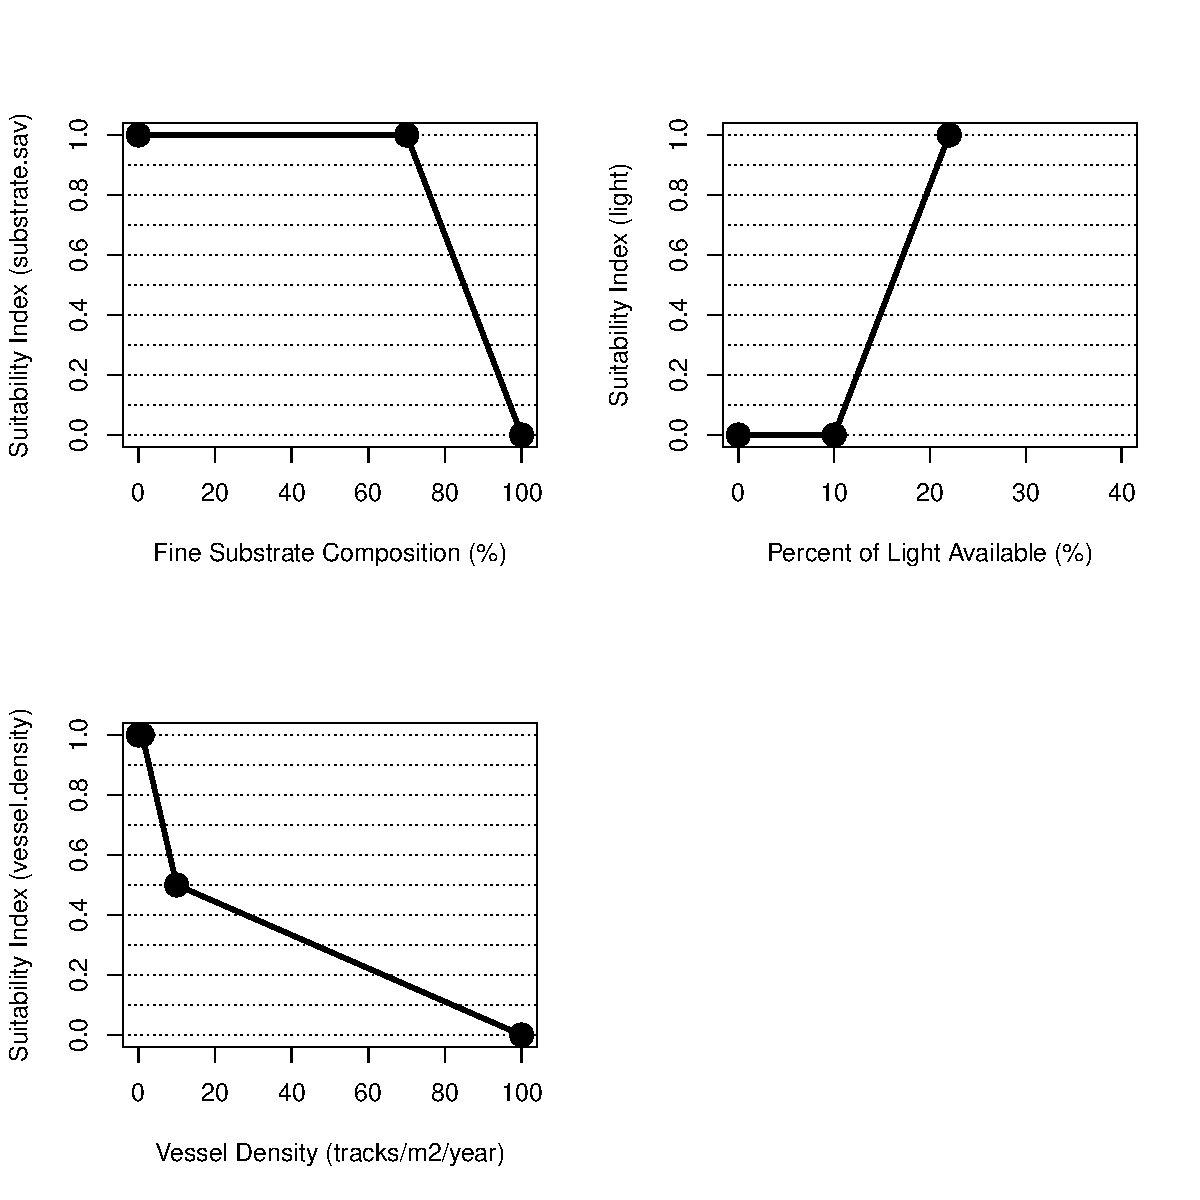
\includegraphics{_main_files/figure-latex/unnamed-chunk-16-1.pdf}
\caption{\label{fig:unnamed-chunk-16}Suitability index curves for hard bottom habitats in the esturaine, subtidal zone.}
\end{figure}

\hypertarget{oyster-substrate}{%
\subsubsection{Oyster Substrate}\label{oyster-substrate}}

Substrate is represented as the percent of the bottom covered with hard substrate, such as existing reefs, or other hard surfaces. We assume that oyster habitat suitability increases linearly from 0 to 100\% cultch cover.

\[cultch = 0.01*hard_{per}\]

Where \(cultch\) is a suitability index relative to hard bottom composition and \(hard_{per}\) is the percent of the substrate that is hard bottom.

\hypertarget{minimum-annual-salinity}{%
\subsubsection{Minimum Annual Salinity}\label{minimum-annual-salinity}}

Minimum Annual Salinity (MAS) is the minimum value of the 12 monthly mean salinities. This variable is essential to describe freshwater impacts (e.g., freshets, high rainfall years, or freshwater diversions) on oysters and is analogous to the frequency of killing floods variable used by \citet{cake_habitat_1983}. For NYBEM, we use a representative low salinity (i.e., the tenth exceedence percentile, \(S_{10}\)) rather than a minimum of monthly average. The relationship between MAS and its suitability index is formulated as a linear step-function as follows:

\[sal.min.ann = \begin{pmatrix} 0.0 & MAS=0-2\\
0.025*MAS-0.05 & MAS=2-4\\
0.225*MAS-0.85 & MAS=4-6\\
0.250*MAS-1.00 & MAS=6-8\\
1.0 & MAS>8
\end{pmatrix}\]

Where \(sal.min.ann\) is a suitability index relative to minimum annual salinity, \(MAS\) is the minimum value of the 12 monthly mean salinities, and \(S_{10}\) is the tenth exceedence percentile of the annual salinity values, a proxy for MAS.

\hypertarget{annual-mean-salinity}{%
\subsubsection{Annual Mean Salinity}\label{annual-mean-salinity}}

Annual Mean Salinity (AS) represents the range of salinities over which adult oysters are viable \citep[@][]{cake_habitat_1983}. The relationship between AS and its suitability index is formulated as a linear step-function as follows:

\[sal.mean.ann = \begin{pmatrix} 0.0 & AS=0-5\\
0.2*AS-1.00 & AS=5-10\\
1.00 & AS=10-15\\
0.08*AS-2.2 & AS=15-20\\
0.07*AS-2.0 & AS=20-25\\
0.03*AS-1.0 & AS=25-30\\
0.01*AS-0.4 & AS=30-40\\
0.0 & AS>40
\end{pmatrix}\]

Where \(sal.mean.ann\) is a suitability index relative to mean annual salinity and \(hard_{per}\) is the percent of the substrate that is hard bottom.

\hypertarget{key-gaps-in-est.sub.hard}{%
\subsubsection{\texorpdfstring{Key Gaps in \texttt{est.sub.hard}}{Key Gaps in est.sub.hard}}\label{key-gaps-in-est.sub.hard}}

This model for hard bottom habitat omits some important variables and processes. Notably, mean Salinity during Spawning Season (MSSS) represents reflects the higher optimal salinities required for spawning and larval stages \citep{butler_summary_1954},\citep[@][]{cake_habitat_1983} and is part of the OHSIM framework but omitted here.

\hypertarget{soft-bottom-habitats-est.sub.soft}{%
\subsection{\texorpdfstring{Soft Bottom Habitats (\texttt{est.sub.soft})}{Soft Bottom Habitats (est.sub.soft)}}\label{soft-bottom-habitats-est.sub.soft}}

Estuarine, subtidal soft bottom habitats comprise large portions of the study areas and host a variety of taxa of interest to environmental management. Specifically, submerged aquatic vegetation (SAV) beds and hard clams are focal targets of management. Specifically, submerged aquatic vegetation (SAV) beds and hard clams are focal target of management. However, these two outcomes have different ecological drivers. As such, the \texttt{est.sub.soft} model represents a hybridized approach that attempts to assess the general condition of this habitat type relative to both major outcomes.

Habitat suitability is assessed separately for SAV and hard clams. The overall habitat suitability of the estuarine, subtidal, soft bottom ecosystem is aggregated into a single metric via a maximum of the separate suitability indices. This approach assumes that a given patch does not need to be perfect for both taxa simultaneously, but instead, the habitat could have high quality relative to one or the other outcome.

\(I_{est.sub.soft} = max({I_{sav},I_{clam})}\)

Where \(I_{est.sub.soft}\) is an overarching index of ecosystem quality for the estuarine, subtidal, soft bottom habitats, \(I_{sav}\) is a suitability index relative to submerged aquatic vegetation, and \(I_{clam}\) is a suitability index relative to hard clams. All indices are quality metrics scaled from 0 to 1, where 0 is unsuitable and 1 is ideal.

\hypertarget{submerged-aquatic-vegetation-module}{%
\subsubsection{Submerged Aquatic Vegetation Module}\label{submerged-aquatic-vegetation-module}}

The SAV submodel is represented by three variables critical for growth and reproduction of seagrass, (1) substrate, (2) light availability, and (3) development stress. Suitability scores are represented either as discrete categories or as step functions with linear interpolations between steps.

\(I_{sav} = \frac{substrate.sav + light + vessel.density}{3}\)

Where \(I_{sav}\) is an overarching index of ecosystem quality relative to submerged aquatic vegetation, \(substrate.sav\)is a suitability index relative to fine substrate, light is a suitability index relative to light penetration, and \(vessel.density\)is a suitability index relative to boat traffic and human uses (a proxy for development stress). All indices are quality metrics scaled from 0 to 1, where 0 is unsuitable and 1 is ideal.

\begin{figure}
\centering
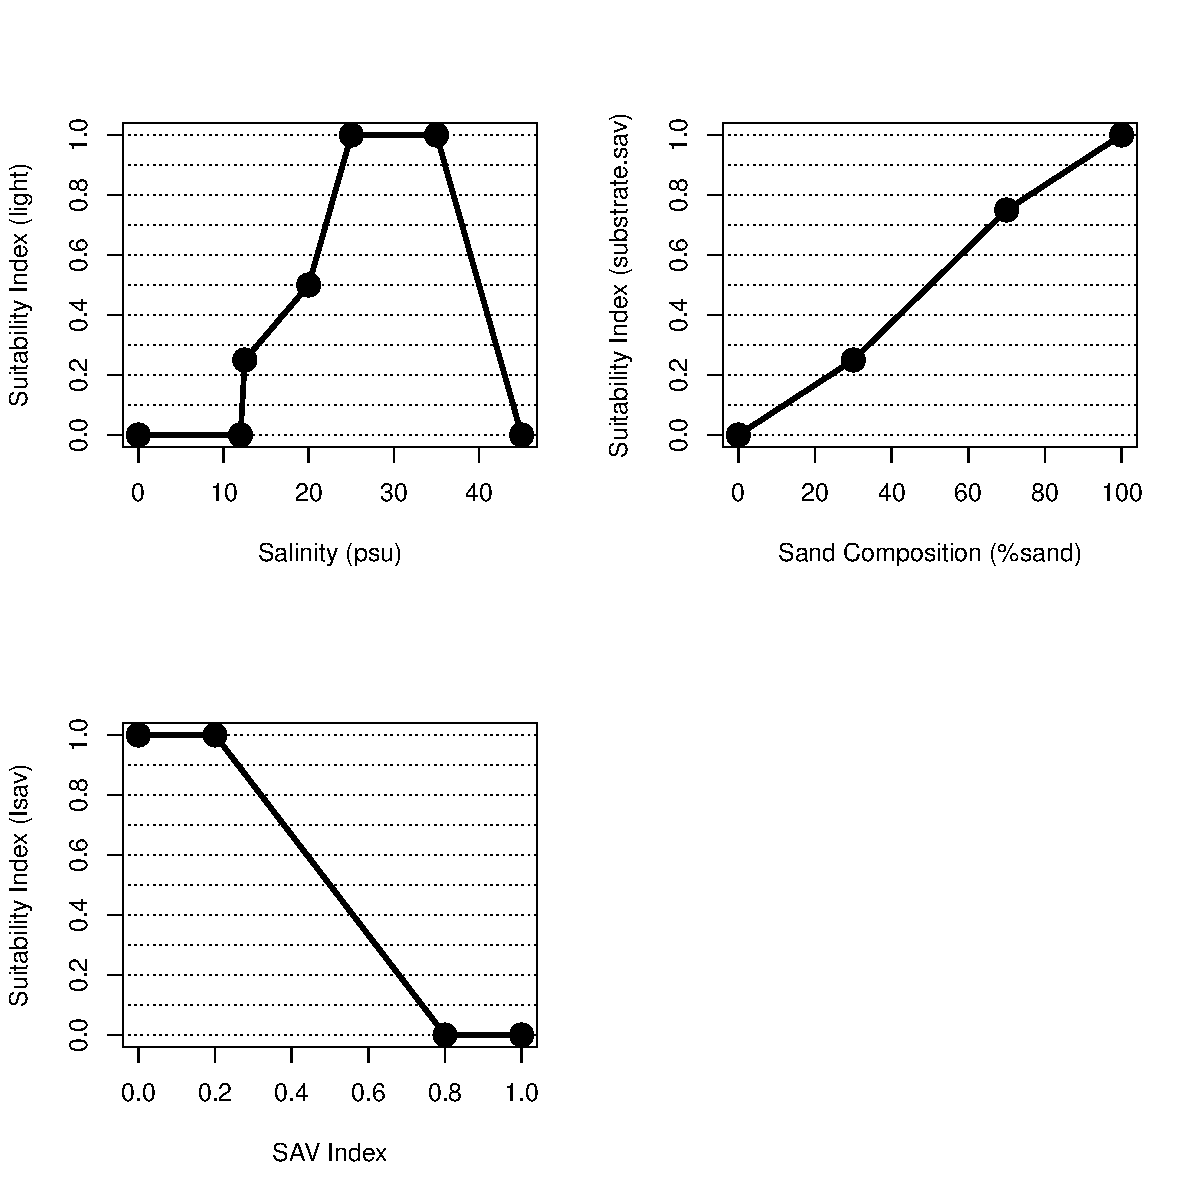
\includegraphics{_main_files/figure-latex/unnamed-chunk-17-1.pdf}
\caption{\label{fig:unnamed-chunk-17}Suitability index curves for seagrass in soft bottom habitats in the esturaine, subtidal zone.}
\end{figure}

Substrate is represented as the presence of soft-bottom sediments conducive for SAV growth. Optimal conditions for growth in the study region were identified as non-cobble substrates with less than 70\% fine sediment. Soft-bottom, non-cobble substrates with greater than 70\% fine sediment were considered sub-optimal/adequate. Suitability scores for SAV substrate are represented as follows:

\[sal.mean.ann = \begin{pmatrix} 1.0 & fines_{per}=0-70\\
-0.033*fines_{per}-3.33 & fines_{per}>70\\
\end{pmatrix}\]

Where \(substrate.sav\) is a suitability index relative to fine substrate and \(fines_{per}\) is the percent of fine substrate (silt and clay).

Light availability drives photosynthesis in SAV. Light attenuates within the water column based on depth and water clarity (i.e., the deeper and more turbid the water, the less light reaches the bottom). For the ESM, light availability depends on depth and Total Suspended Solids (TSS) and is calculated algorithmically, then converted into a suitability index. Light availability (Iz) at the plant surface is estimated based on \citet{van_nes_charisma_2003} is calculated in Equations 34-35 as follows:

\[I_{z} = PAR * exp(-K_{d}*z)\]

where \(PAR\) represents the photosynthetically active radiation at the surface, \(K_{d}\) is the light attenuation coefficient for water clarity matching the conditions of the study site, and \(z\) is water depth.

Light at the plant surface is converted to a percent of light available at that depth, which is used to calculate a suitability score.

\[PLW = \frac{I_{z}}{PAR} * 100\]

The relationship between Percent light available (PLA) and its suitability index for SAV is represented as follows:

\[light = \begin{pmatrix} 0.0 & PLA<10\\
0.0833*PLA-0.83 & PLA>70\\
1.0 & PLA>22\\
\end{pmatrix}\]

Where \(light\) is a suitability index relative to light penetration and \(vessel.density\) is a suitability index relative to boat traffic and human uses.

Human-mediated disturbances (e.g., urban development, increased vessel traffic, etc.) can negatively impact SAV abundance. We quantify these disturbances through a proxy of vessel traffic per area. Vessel traffic is obtained from the Automatic Identification System database. Lower traffic (less than 10 tracks per year) is optimal and the suitability decreases with increasing vessel traffic. Suitability scores for are quantified as follows:

\[vessel.density = \begin{pmatrix} 1.0 & ves_{AIS}=0-1\\
-0.0556*ves_{AIS}+1.06 & ves_{AIS}=1-10\\
-0.00556*ves_{AIS}+0.56 & ves_{AIS}=10-100\\
0.0 & ves_{AIS}>100
\end{pmatrix}\]

Where \(vessel.density\) is a suitability index relative to ship traffic and \(ves_{AIS}\) is the vessel density from the Automated Information System.

\hypertarget{hard-clam-module}{%
\subsubsection{Hard Clam Module}\label{hard-clam-module}}

The clam habitat suitability submodel is based on \emph{Thompson et al.~(2021)}. Ideal depth for hard clams has been reported as 4 to 8 m, however hard clams can be found in shallower depths, but the habitat is considered suboptimal. This submodel consists of three variables (1) salinity, (2) substrate, and (3) SAV suitability.

\(I_{clam} = \frac{salinity.clam + substrate.clam + sav.prob}{4}\)

Where \(I_{clam}\) is an overarching index of ecosystem quality relative to hard clam habitat, \(salinity.clam\) is a suitability index relative to salinity, \(substrate.clam\) is a suitability index relative to fine substrate, and \(sav.prob\) is an overarching index of ecosystem quality relative to submerged aquatic vegetation coverage. All indices are quality metrics scaled from 0 to 1, where 0 is unsuitable and 1 is ideal.

\begin{figure}
\centering
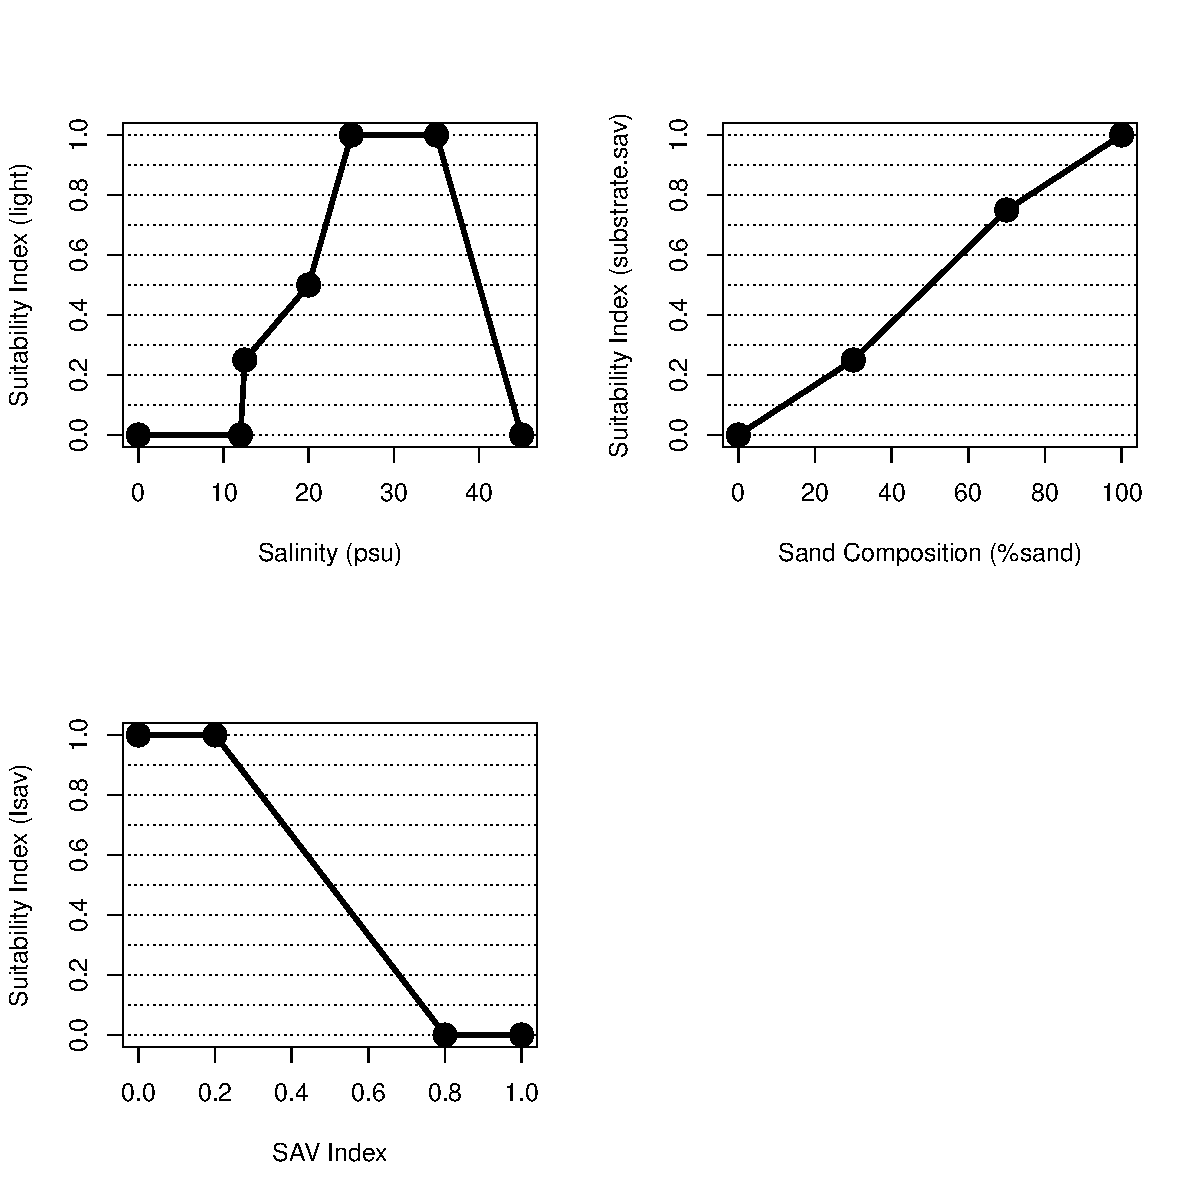
\includegraphics{_main_files/figure-latex/unnamed-chunk-18-1.pdf}
\caption{\label{fig:unnamed-chunk-18}Suitability index curves for clams in soft bottom habitats in the esturaine, subtidal zone.}
\end{figure}

Salinity represents the range of salinities over which clams can survive. Optimal salinity for hard clams ranges from 25 to 35 psu. Hyper- and hypo-saline conditions (\textgreater{} 45 or \textless12.5 psu, respectively) are considered unsuitable when clams are exposed to these conditions for three to six consecutive days. Habitat suitability increases with increasing salinity for intermediate values. The relationship between salinity and its suitability index is formulated as follows:

\[salinity.clam = \begin{pmatrix} 0.0 & salinity.psu=0-12\\
0.5*salinity.psu-6.0 & salinity.psu=12-12.5\\
0.033*salinity.psu-0.17 & salinity.psu=12.5-20\\
0.1*salinity.psu-1.5 & salinity.psu=20-25\\
1.0 & salinity.psu=25-35\\
-0.1*salinity.psu+4.5 & salinity.psu=12.5-20\\
0.0 & salinity.psu>45
\end{pmatrix}\]

Where \(salinity.clam\) is a suitability index relative to salinity and \(salinity.psu\) is mean annual salinity.

Similar to seagrass and oysters, substrate is a critical parameter for hard clam viability. Optimal substrate is shelly soft bottom. As the substrate composition increases in sand and/or mud, the substrate is less suitable for clams. Suitability scores for clam substrate are quantified as follows:

\[substrate.clam = \begin{pmatrix} 0.0083*sand_{per} & sand_{per}=0-30\\
0.0125*sand_{per}-0.13 & sand_{per}=30-70\\
0.0083*sand_{per}+0.17 & sand_{per}=70-100
\end{pmatrix}\]

Where \(substrate.clam\) is a suitability index relative to fine substrate and \(sav.prob\) is sand composition of the substrate (\%sand).

Optimal habitat for hard clams is sandy bottom without seagrass. As seagrass coverage increases, the suitability for clams decreases. As a proxy for seagrass coverage, we use the index of seagrass suitability (\(I_{clam}\)). The relationship between seagrass suitability and hard clam suitability is formulated as follows:

\[sav.prob = \begin{pmatrix} 1.0 & I_{sav}=0-0.2\\
-1.667*I_{sav}+1.33 & I_{sav}=0.2-0.8\\
0.0 & I_{sav}=0.8-1.0
\end{pmatrix}\]

Where \(sav.prob\) is an overarching index of ecosystem quality relative to submerged aquatic vegetation coverage and \(I_{clam}\) is an overarching index of ecosystem quality relative to submerged aquatic vegetation coverage.

\hypertarget{potential-extension-of-estuarine-subtidal-model}{%
\subsubsection{Potential extension of estuarine, subtidal model}\label{potential-extension-of-estuarine-subtidal-model}}

This model for soft bottom habitat omits some important variables and processes. Notably, temperature is not presently included but represents a crucial variable for both SAV and clams.

\begin{itemize}
\item
  \emph{Temperature for SAV}: Like all vascular plants, temperature is a major driver for SAV viability. At low temperatures, physiological processes are constrained, while metabolic temperature increases with higher temperatures (Staehr et al.~2011).At temperatures above optimal range for SAV, metabolic activity is significantly reduced or halted as a result of protein denaturation or inactivation \citep{atkin_thermal_2003};\citep{jensen_psi-k_2000}.
\item
  \emph{Temperature for Clams}: Temperature for Clams: Water temperature can have significant impacts on hard clams. For future models, temperatures below biological zero (5°C) and above 33°C are likely unsuitable. Temperatures between 12.5°C and above 32°C range in suitability with optimal temperatures between 22.5°C and 30°C.
\end{itemize}

\hypertarget{marine-intertidal-zone}{%
\section{Marine, Intertidal Zone}\label{marine-intertidal-zone}}

Marine, intertidal ecosystems include the areas of high salinity (\textgreater{} 30 psu) bracketed by tidal limits of the mean higher high water (MHHW) and mean lower low water (MLLW). In the context of NYBEM, these systems tend to directly front the Atlantic Ocean as beaches or occur in high salinity zones near inlets.

Figure XX presents a conceptual model of the marine, intertidal ecosystem. This nearshore ecosystem is strongly influenced by two major pressures, the physical drivers of the ocean environment (e.g., currents, sediment transport) and human uses of the system (e.g., beaches and associated upland development). Ecologically, this ecosystem hosts a variety of species of management interest such as seabeach amaranth, horseshoe crabs, shorebirds (e.g., piping plover, terns, red knot), and sea turtles.

Coastal storm risk management actions have the potential to affect this ecosystem through two primary mechanisms. First, some risk management actions (e.g., storm surge barriers) could be directly constructed in this area. Second, large-scale features have the potential to alter coastal dynamics indirectly, although this affect may occur to a lesser extent given the overarching dominance of ocean effects.

\begin{figure}
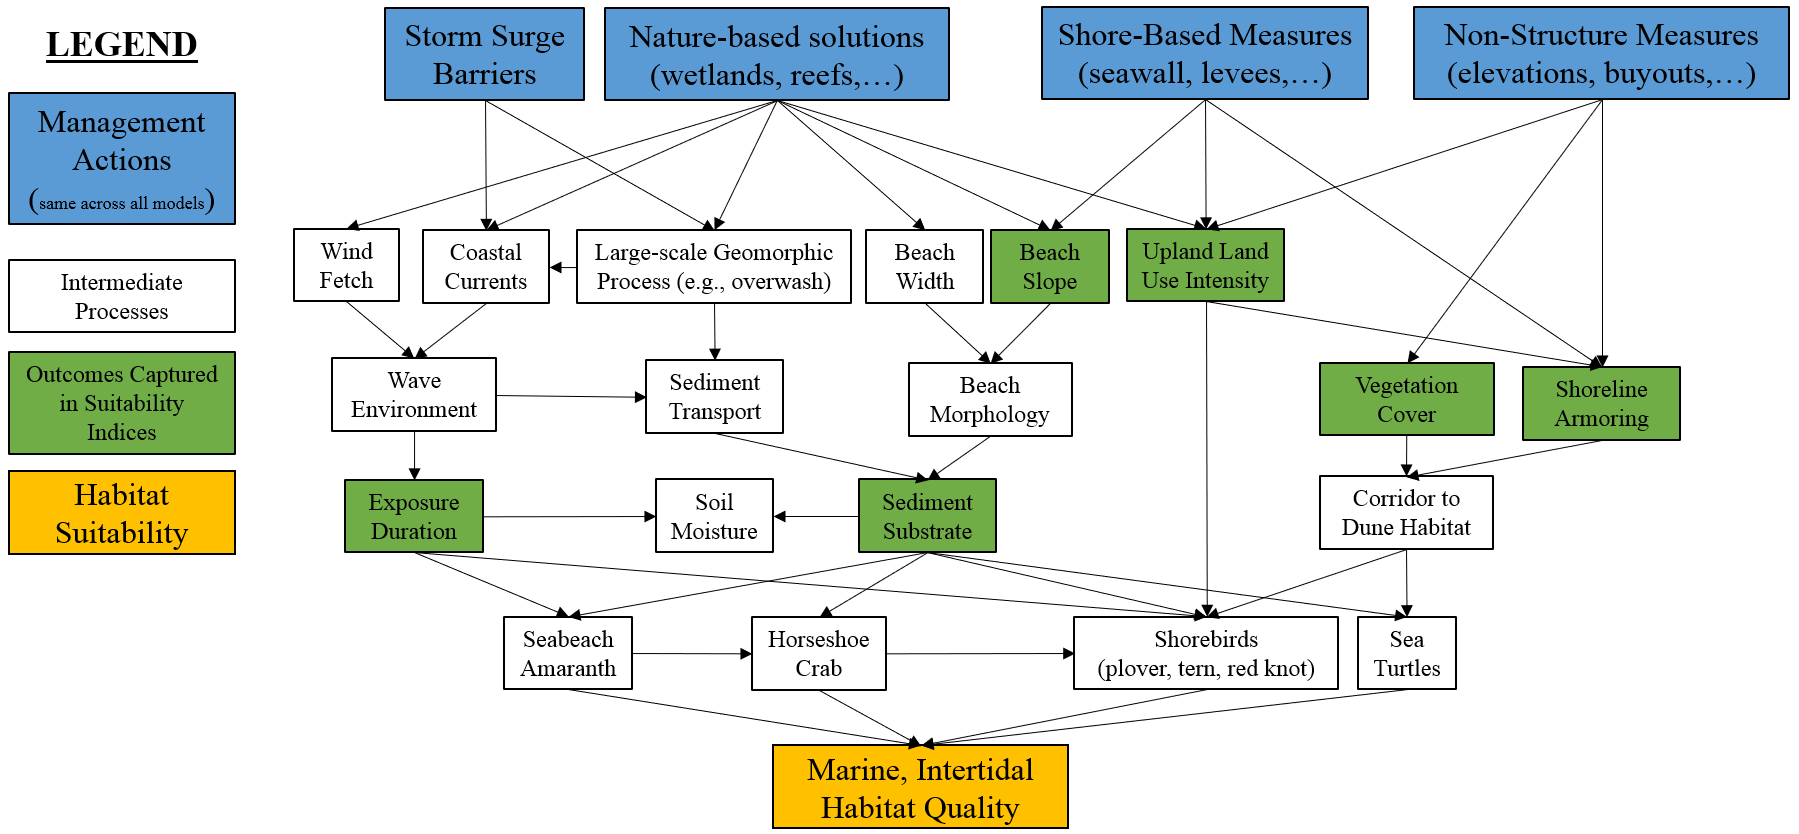
\includegraphics[width=24.99in]{ZZ_Fig04.10_Mar.Int_ConModel} \caption{Conceptual model for the marine, intertidal submodel.}\label{fig:unnamed-chunk-19}
\end{figure}

The tension between human uses of this landscape and ecological outcomes has long been acknowledged, and many models have been developed to assess ecological outcomes in marine, intertidal zones of the region. This submodel drew heavily from four general bodies of knowledge, specifically:

\begin{itemize}
\item
  USFWS Habitat Evaluation Procedure models: tern \citep{carreker_habitat_1985}, \citep{us_fish_and_wildlife_service_usfws_gulf_2001}, plover \citet{us_fish_and_wildlife_service_usfws_gulf_2001}, horseshoe crab \citet{us_fish_and_wildlife_service_usfws_gulf_2001}, red knot \citet{us_fish_and_wildlife_service_usfws_gulf_2001}.
\item
  Other habitat suitability models: plover (\citet{farmer_habitat_2000}, \citet{seavey_effect_2011}), horseshoe crab \citep{avissar_modeling_2006}, \citep{nancy_jackson_armoring_2010}, {[}Lathrop\_2013{]}, amaranth \citep{sellars_habitat_2007}, sea turtles \citep{dunkin_spatially_2016}\\
\item
  Fire Island to Montauk Point Habitat Evaluation Procedure OceanBeach Sub-Model \citep{usace_evaluation_2009}.\\
\item
  Empirical studies of the system: Virginia Tech shorebird program \citep{herman_unpacking_2019}, Rutgers horseshoe crab mapping \citep{lathrope_mapping_2013}, international shorebird survey (Manomet)
\end{itemize}

Four classes of processes and dynamics were identified from a review of these models and studies: long-term and large-scale wave and sediment dynamics, beach morphology, benthic food supplies, and the role of this system as a corridor between aquatic and upland environments. From these processes, six surrogate metrics were identified, which collectively reflect the condition of the marine, intertidal zone. Notably, variables reflecting wave and sediment dynamics are minimally included in this phase of modeling due to assessment challenges. The sections below describe each metric and the rationale in detail, but briefly:

\begin{itemize}
\item
  Beach slope was identified as a proxy for larger effects on overall morphology and grain size.
\item
  The proportion of time a beach is exposed provides a metric of benthic food supplies and availability of foraging habitat.
\item
  Upland land use intensity and shoreline armoring metrics describe the general human use pressures on a given system and viability of corridor functions.
\item
  A vegetation cover metric assesses the viability of the corridor relative to different taxa movement requirements.
\end{itemize}

The overall habitat suitability of the marine, intertidal zone may then be aggregated into a single metric via an arithmetic mean of suitability indices for these six metrics.

\(I_{mar.int} = \frac{beach.slope + exp.dur + substrate + land.use + veg.cover + shoreline}{6}\)

Where \(I_{mar.int}\) is an overarching index of ecosystem quality for the marine intertidal zone, \(beach.slope\) is a suitability index relative to beach slope, \(exp.dur\) is a suitability index relative to the duration of beach exposure, \(substrate\) is a suitability index relative to fine substrate, \(land.use\) is a suitability index relative to adjacent upland land uses, \(veg.cover\) is a suitability index relative to vegetative cover, and \(shoreline\) is a suitability index relative to shoreline armoring. All indices are quality metrics scaled from 0 to 1, where 0 is unsuitable and 1 is ideal.

\begin{figure}
\centering
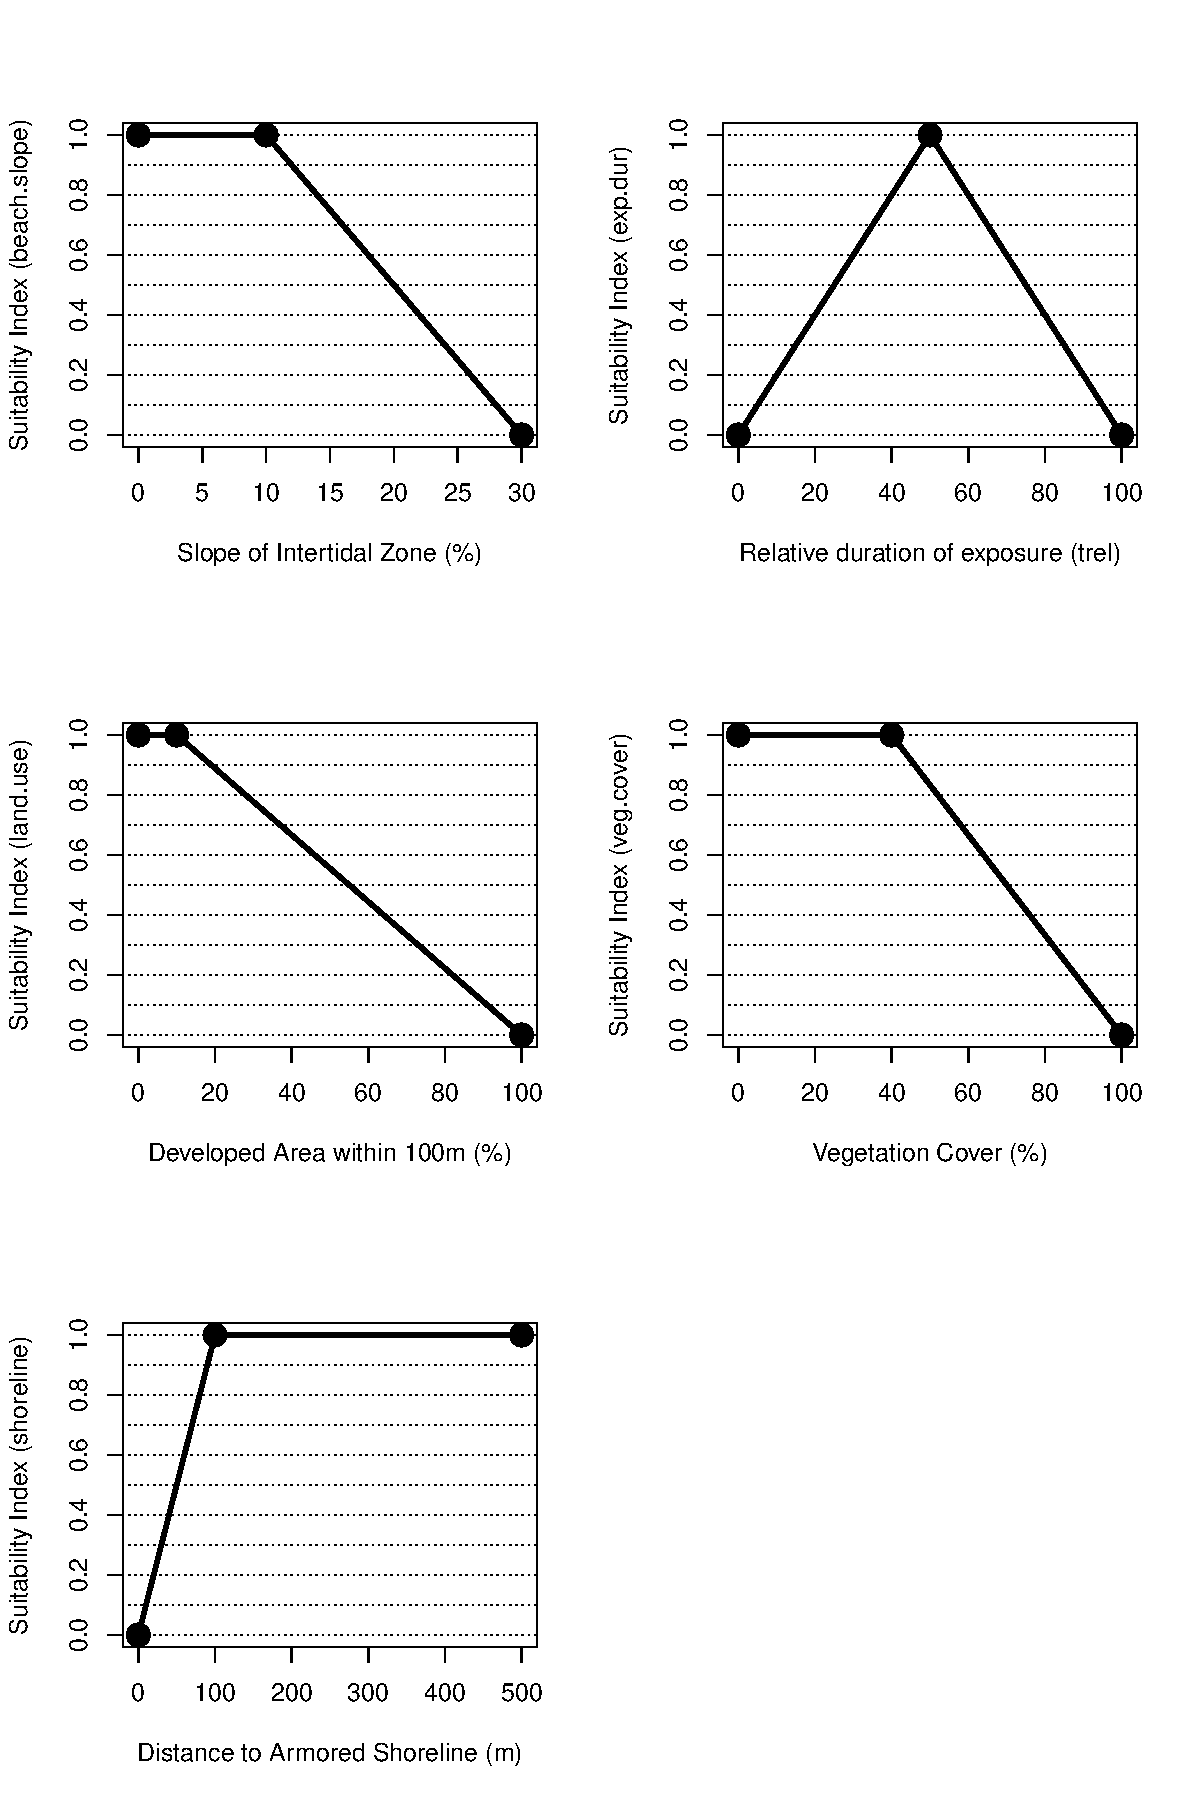
\includegraphics{_main_files/figure-latex/unnamed-chunk-20-1.pdf}
\caption{\label{fig:unnamed-chunk-20}Suitability index curves for the marine, intertidal zone.}
\end{figure}

\hypertarget{beach-slope}{%
\subsection{Beach Slope}\label{beach-slope}}

Beach morphology directly affects habitat use by multiple focal taxa (e.g., shorebirds, turtles, horseshoe crab). Beach shape and morphologic character can be described through parameters of width, slope, elevation, and other summaries of topography \citep{bridges_use_2015}. Beach width is indirectly captured in NYBEM through metrics of habitat quantity and patch size and is not considered here. Beach slope integrates morphologic outcomes and is directly tied to grain size and wave environment \citep{lodder_chapter_2021}. Beach slope, thus, provides an important and synthetic metric of marine, intertidal habitat quality.

Beach slope is identified as a general indicator of ecosystem condition for Long Island ecosystems (\citet{usace_evaluation_2009}), and as an important driving component of habitat use by multiple taxa in the New York Bight. For example, seabeach amaranth (\emph{Amaranthus pumilus}) typically occurs in low slope environments \citep{sellars_habitat_2007}), while habitat is most suitable for horseshoe crabs between \textasciitilde5-10\% slopes \citep{brady_habitat_1996}. Notably, not all taxa may respond in kind to these generalization; for instance, sea turtles have shown habitat preferences for moderate slopes between \textasciitilde10-30\% in subtropical areas such as Southeastern Florida. Beach slope, thus, provides an important and synthetic metric of marine, intertidal habitat quality. Merging these regional models, NYBEM assesses suitability relative to beach slope as follows:

\[beach.slope = \begin{pmatrix} 1.0 & slope_{per}=0-10\\
-0.05*slope_{per}+1.5 & slope_{per}=10-30\\
0.0 & slope_{per}>30
\end{pmatrix}\]

Where \(beach.slope\) is a suitability index relative to beach slope and \(slope_{per}\) is the slope of the beach perpendicular to the mean tide line in percent.

\hypertarget{exposure-duration}{%
\subsection{Exposure Duration}\label{exposure-duration}}

Intertidal zones are a key foraging habitat for shorebirds. The benthic food availability is related in part to soil moisture \citep{brady_habitat_1996} and the time to forage in these zones. Soil moisture is also a key determinant of horseshoe crab spawning \citep{avissar_modeling_2006}. For NYBEM, a proxy variable is used to account for these processes. Specifically, a ratio of depth ranges to the tidal range is used as a relative duration of exposure, which we calculate as follows:

\[t_{rel} = \frac{H_{max} - H_{min}}{MHHW-MLLW}\]

Where \(t_{rel}\) is a relative duration of exposure, \(H_{max}\) is the maximum depth observed over a hydrodynamic simulation period, \(H_{min}\) is the minimum depth observed over a hydrodynamic simulation period, \(MHHW\) is mean higher high water, and \(MLLW\) is mean lower low water.

This metric provides a relative accounting for the amount of exposure a given path experiences. For instance, \(t_{rel}>1\) occurs in portions of the intertidal that remain underwater most of the time, and \(t_{rel}=0\) occurs in areas where the elevation exceeds the intertidal range. In terms of habitat suitability, we assume that ideal values of this metric occur around 0.5 (near the mean tide level) and suitability declines on either side of this threshold as follows:

\[exp.dur = \begin{pmatrix} 0.02*t_{rel} & t_{rel}<0.5\\
-0.02*t_{rel}+2 & t_{rel}>0.5\\
0.0 & t_{rel}>1.0
\end{pmatrix}\]

Where \(exp.dur\) is a suitability index relative to exposure duration.

\hypertarget{upland-land-use}{%
\subsection{Upland Land Use}\label{upland-land-use}}

Marine, intertidal zones are a key transitional habitat between aquatic and upland systems. Fully functional intertidal areas would include high-quality adjacent uplands and subtidal areas. A variety of metrics have been used to assess human impacts on this system, including diverse metrics like foot traffic, vehicle use of beaches, beach grooming and maintenance practices, physical barriers along the beach \citep{farmer_habitat_2000}; direct human development such as buildings; trash and debris presence \citep{usace_evaluation_2009}; and general levels of land use intensity \citep{seavey_effect_2011}.

For the NYBEM, habitat suitability is modeled based on a relative metric of development for adjacent uplands within 100m. When the percentage of developed adjacent uplands is greater than 10\%, habitat suitability in the estuarine intertidal ecosystem declines. When the development of adjacent upland reaches 100\% of the estuarine intertidal ecosystem, the habitat will no longer be considered suitable.

\[land.use = \begin{pmatrix} 1.0 & urban_{per}=0-10\\
-0.011*urban_{per}+1.11 & urban_{per}=10-100
\end{pmatrix}\]

Where \(land.use\) is a suitability index relative to adjacent upland land uses and \(urban_{per}\) is the percent of adjancent upland in developed (i.e., urban) land uses within 100m.

\hypertarget{vegetation-cover-1}{%
\subsection{Vegetation Cover}\label{vegetation-cover-1}}

Vegetative cover in the intertidal zone produces both positive and negative ecological effects. Animal movement can be disrupted by the presence of vegetation, such as the precipitous declines in habitat suitability for least tern beyond 20-25\% herbaceous or shrub canopy cover \citep{carreker_habitat_1985}. Conversely, vegetation can be a positive attribute and a key transitional feature moving upland toward dune environments, as well as define the difference between the lower intertidal (below MTL) and higher intertidal (above MTL)\citep{usace_evaluation_2009}.

\textbf{REVISIT THIS SUITABILITY CURVE BASED ON GULF OF MAINE MODELS.}

For NYBEM, these competing outcomes are balanced by extending the range of suitable habitat to sparse coverage of 40\% with subsequent declines as vegetation becomes dense. This parameter is assessed through the region based on nationally available Landfire data for existing vegetation cover. Suitability indices are computed as follows:

\[veg.cover = \begin{pmatrix} 1.0 & cover_{per}=0-40\\
-0.0167*cover_{per}+1.67 & cover_{per}=40-100
\end{pmatrix}\]

Where \(veg.cover\) is a suitability index relative to vegetation coverage and \(cover_{per}\) is the percent of vegetation coverage.

\hypertarget{shoreline-armoring-1}{%
\subsection{Shoreline Armoring}\label{shoreline-armoring-1}}

Intertidal areas provide important habitat corridors for organism movement. However, shoreline armoring such as bulkheads or revetments can inhibit movement of the resident taxa (as well as the ecosystem migrating inland with sea level change). Numerous authors have highlighted the negative role that shoreline armoring can play in marine intertidal systems (\citet{usace_evaluation_2009}; \citet{lathrope_mapping_2013}). Ideal habitat suitability would occur in the absence of shoreline armoring, but many shorelines are extensively hardened in the developed New York Bight region.

For NYBEM, the distance to the nearest armored shoreline is used as a relative measure of habitat suitability. Habitat is considered more suitable with increasing distance to armoring. NOAA's \href{https://response.restoration.noaa.gov/resources/environmental-sensitivity-index-esi-maps}{Environmental Sensitivity Index (ESI)} contains mapped extent of shoreline armoring and is used to assess presence or absence consistently across the region. A suitability index is then assessed as follows:

\[shoreline = \begin{pmatrix} 0.01*dist_{armor} & dist_{armor}=0-100m\\
1.0 & dist_{armor}>100m
\end{pmatrix}\]

Where \(shoreline\) is a suitability index relative to shoreline armoring and \(dist_{armor}\) is the distance to the nearest armored shoreline in meters.

\hypertarget{potential-extension-of-marine-intertidal-models}{%
\subsection{Potential extension of marine, intertidal models}\label{potential-extension-of-marine-intertidal-models}}

The \texttt{mar.int} model represents trade-offs between habitat needs for multiple taxa and availability of data at regional scales. Future model development could be expanded to include more processes and outcome, specifically:

\begin{itemize}
\tightlist
\item
  Some authors have distinguished the difference in the upper, vegetated intertidal zone and the lower, unvegetated areas \citep{usace_evaluation_2009}.\\
\item
  Substrate is a key driver of beach outcomes in many contexts \citep{lodder_chapter_2021}, and specifically, substrate is often included in regional models of this system (e.g., \citet{brady_habitat_1996}, \citet{avissar_modeling_2006}). However, high quality substrate data were unavilable, which created a major data gap for incorporating this variable.\\
\item
  Other assessment procedures (\citet{farmer_habitat_2000}, \citet{usace_evaluation_2009}) have included a variety of human development pressures related to local features (e.g., vehicle and foot traffic), which could provide important refinement of the human use intensity metrics for land use and shoreline development.\\
\item
  Wave environments clearly affect the morphology of beaches, and additional hydrodynamic variables could be assessed in future models.
\end{itemize}

\hypertarget{marine-subtidal-zone}{%
\section{Marine, Subtidal Zone}\label{marine-subtidal-zone}}

Marine, subtidal ecosystems include the areas of high salinity (\textgreater{} 30 psu) bracketed by tidal limits of the mean lower low water (MLLW) and 2m below Mean Tide Level (MTL). In the context of NYBEM, these systems tend to directly front the Atlantic Ocean as beaches or occur in high salinity zones near inlets.

Figure XX presents a conceptual model of the marine, subtidal ecosystem. This nearshore ecosystem hosts a variety of species of management interest such as hard clams, winter flounder, and seagrasses. As such, this model generally centers on the pelagic systems, submerged aquatic vegetation, and the benthic system. In general, coastal storm risk management actions are more likely to have direct effects on this ecosystem (e.g., footprint of constructed storm surge barriers) than indirect, offsite concerns more common in the estuarine systems.

\begin{figure}
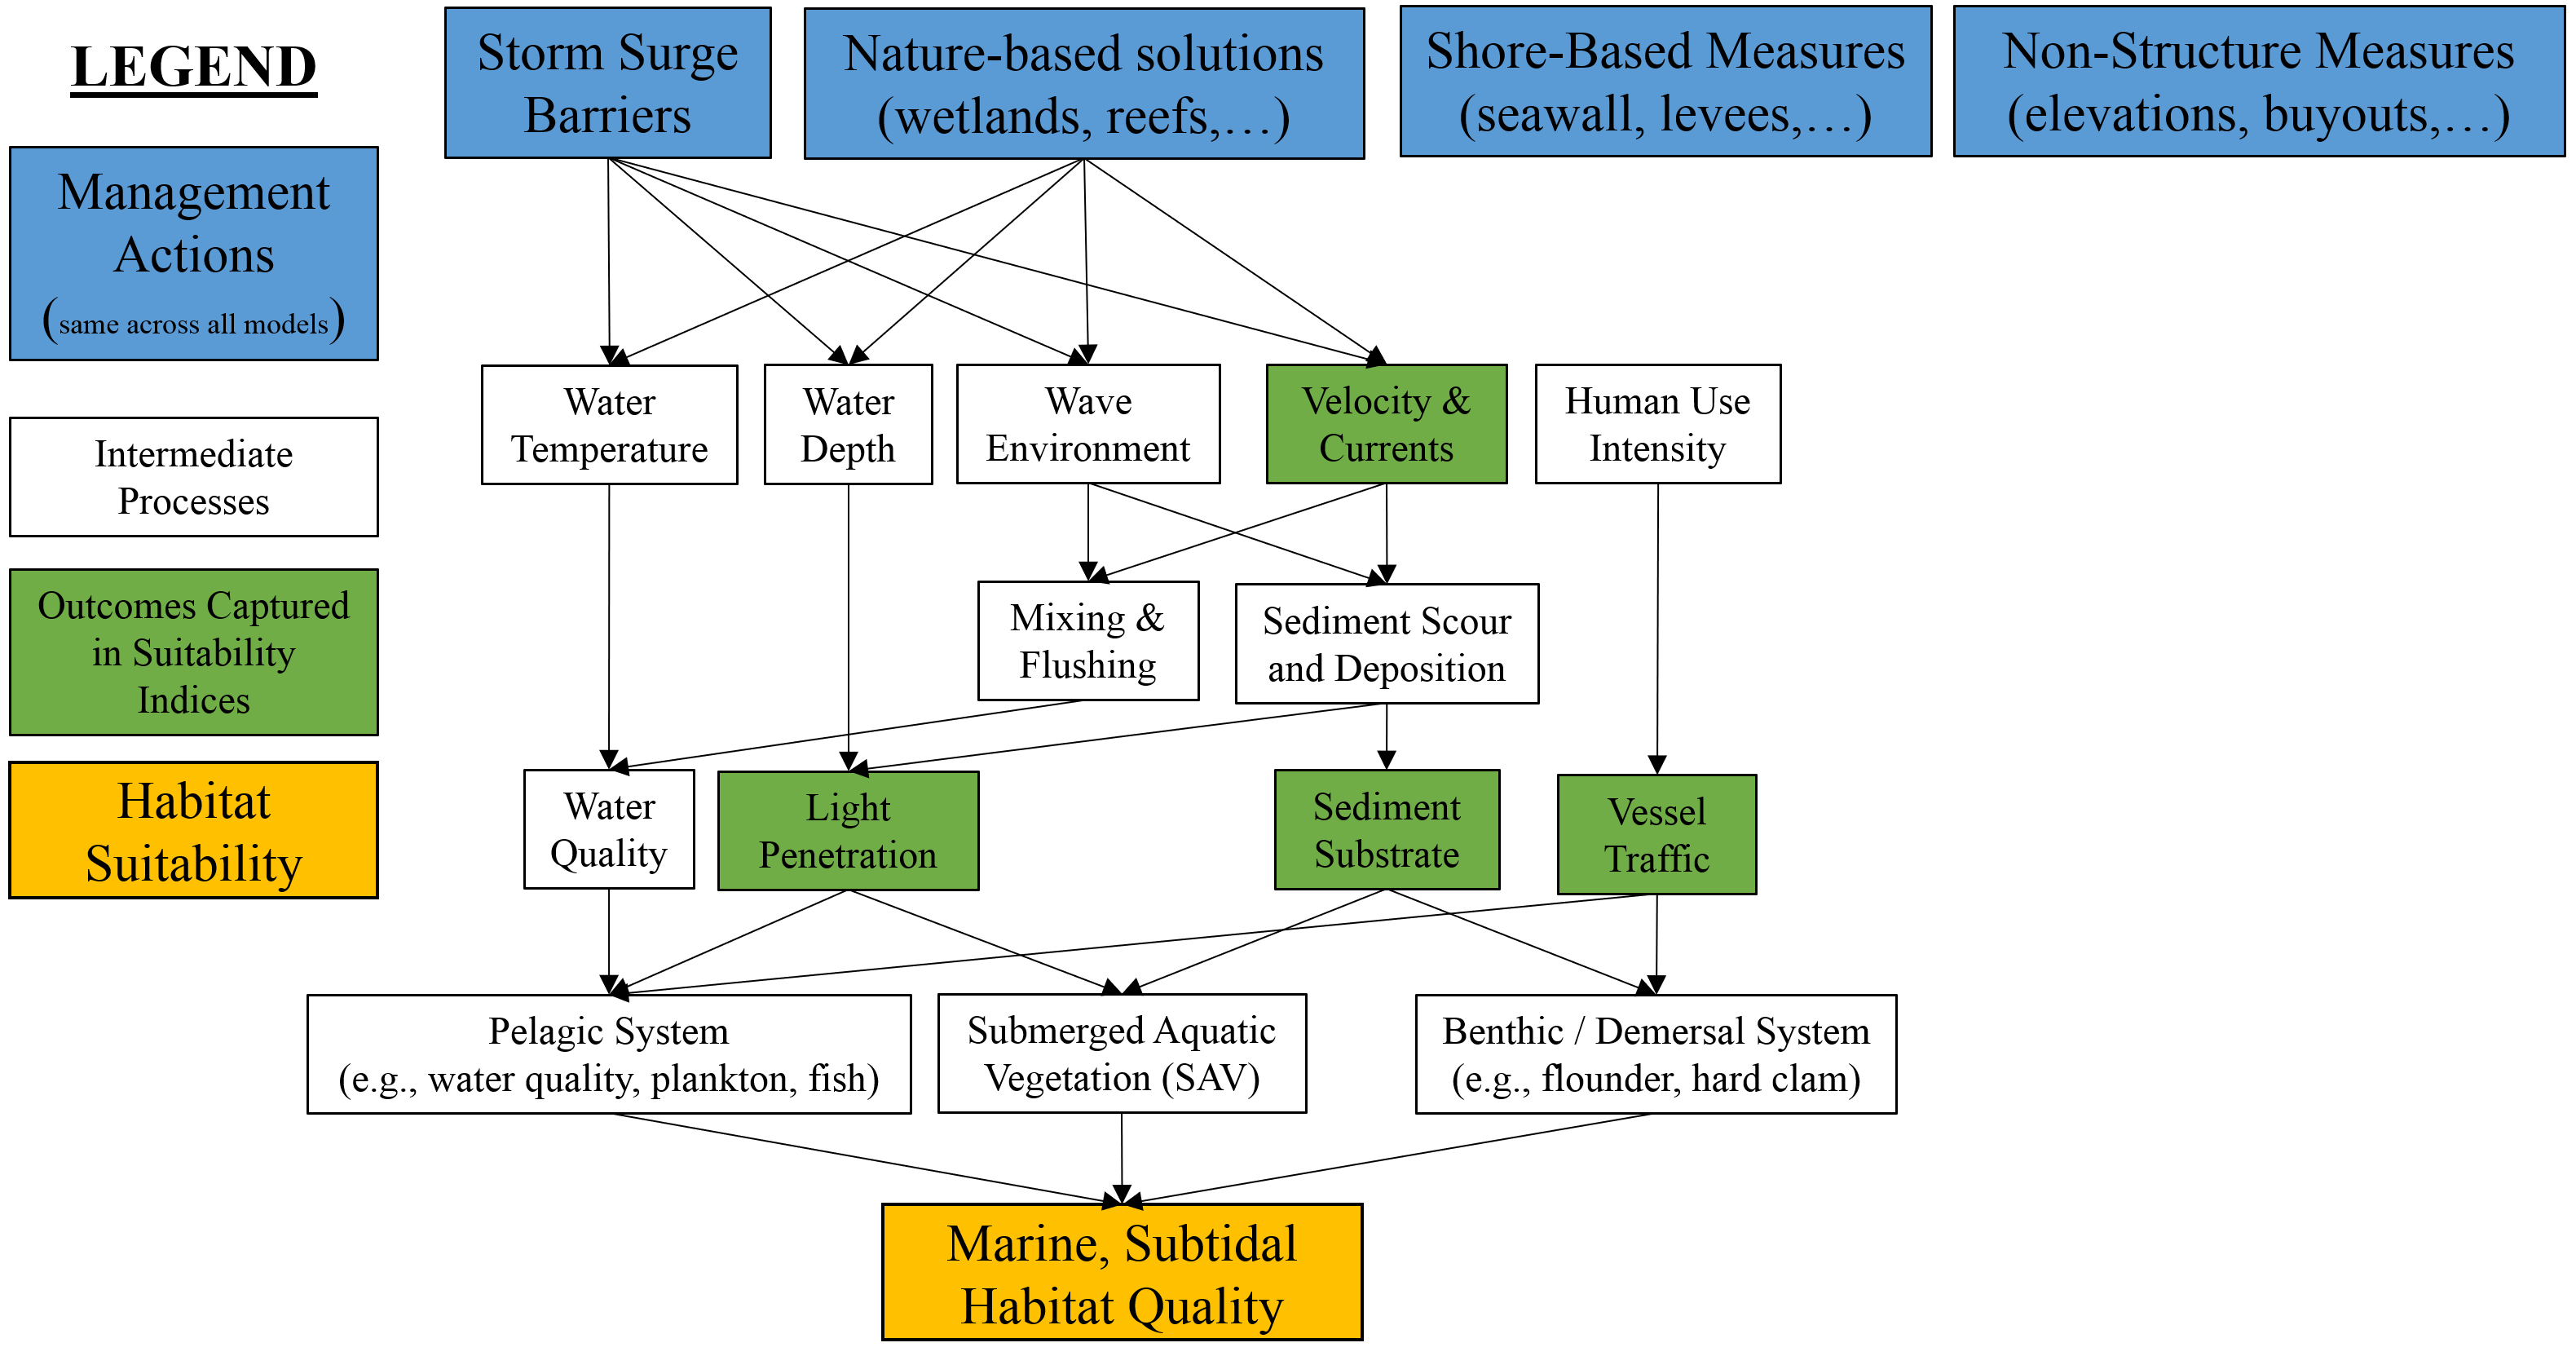
\includegraphics[width=43.89in]{ZZ_Fig04.12_Mar.Sub_ConModel} \caption{Conceptual model for the marine, subtidal submodel.}\label{fig:unnamed-chunk-21}
\end{figure}

The tension between human uses of this landscape and ecological outcomes has long been acknowledged, and many models have been developed to assess ecological outcomes in marine, subtidal zones of the region. This submodel drew heavily from three primary bodies of knowledge, specifically:

\begin{itemize}
\item
  NY/NJ harbor mitigation functional assessment models \citep{usace_new_2000}
\item
  Habitat suitability models for winter flounder\citep{banner_usfws_2001}, and hard clam \citep{mulholland_habitat_1984-1}.
\item
  Regional monitoring data associated with NY/NJ Harbor Deepening (\citet{usace_application_2012}, \citet{usace_demersal_2015a}, \citet{usace_dredge_2015b}), essential fish habitat mapping \citep{usace_essential_2013}, and water quality data for the lower bay (DEP 2018, \citet{usace_dredge_2015b}).
\end{itemize}

Four main classes of processes and dynamics were identified from a review of these models and studies: a) substrate-driven habitat use, b) physical currents and mixing, c) light penetration, and d) human uses of the system. From these processes, four surrogate metrics were identified, which collectively reflect the condition of the marine, subtidal zone. The sections below describe each metric and the rationale in detail, but briefly:

\begin{itemize}
\item
  Current velocity is a major driver of sediment dynamics as well as water quality processes.
\item
  Fine substrate affects utilization of habitats by a variety of taxa.
\item
  Light penetration is a proxy for both water quality outcomes and potential for SAV growth.
\item
  Vessel traffic density as a proxy for human use intensity.
\end{itemize}

The overall habitat suitability of the marine, subtidal zone may then be aggregated into a single metric via an arithmetic mean of suitability indices for these four metrics.

\(I_{mar.sub} = \frac{velocity + substrate + light + vessel.density}{4}\)

Where \(I_{mar.sub}\) is an overarching index of ecosystem quality for the marine subtidal zone, \(velocity\) is a suitability index relative to beach slope, \(substrate\) is a suitability index relative to fine substrate, \(light\) is a suitability index relative to light penetration, and \(vessel.density\) is a suitability index relative to boat traffic and human uses. All indices are quality metrics scaled from 0 to 1, where 0 is unsuitable and 1 is ideal.

\begin{figure}
\centering
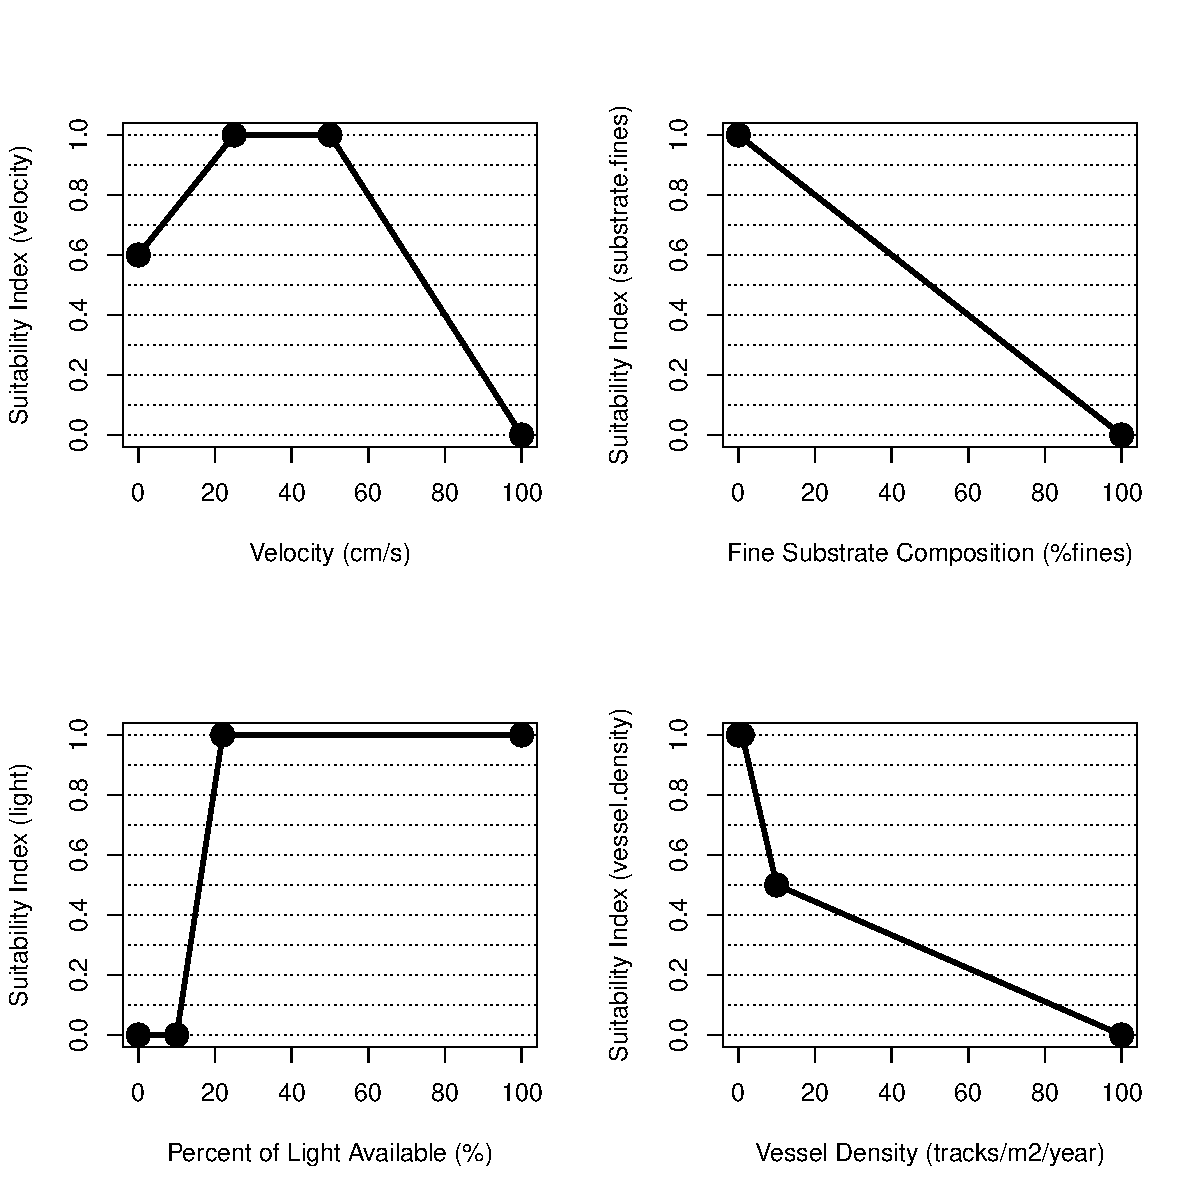
\includegraphics{_main_files/figure-latex/unnamed-chunk-22-1.pdf}
\caption{\label{fig:unnamed-chunk-22}Suitability index curves for the marine, deepwater zone.}
\end{figure}

\hypertarget{velocity}{%
\subsection{Velocity}\label{velocity}}

Velocity, currents, and wave environment are a key determinant of habitat suitability as well as critical drivers of sediment dynamics and water quality processes. For example, hard clam habitat suitability is generally in low to moderate velocity environments (\textless50 cm/s) with declines in suitability up to 100 cm/s. For NYBEM, the velocity suitability for hard clams is adopted directly from \citet{mulholland_habitat_1984-1} as shown below. We assess velocity as the median velocity observed over an annual hydrodynamic simulation.

\[velocity = \begin{pmatrix} 0.016*V_{50}+0.6 & V_{50}=0-1\\
1.0 & V_{50}=1-10\\
-0.02*ves_{AIS}+2 & V_{50}=10-100\\
0.0 & V_{50}>100
\end{pmatrix}\]

Where \(velocity\) is a suitability index relative to currents and velocity and \(ves_{AIS}\) is the vessel density from the Automated Information System.

\hypertarget{substrate}{%
\subsection{Substrate}\label{substrate}}

Sediment quality drives multiple aspects of ecosystem integrity such as benthic habitat provision, nutrient dynamics, and erodibility. Fine sediment composition (i.e., \%fine) is a common metric in multiple assessment procedures in the region (e.g., \citet{mulholland_habitat_1984-1}, \citet{usace_new_2000}, \citet{USACE_port_2021}). Specifically, the suitability curves from the hard clam model \citep{mulholland_habitat_1984-1} are adopted here as a rapid metric of ecosystem quality. For marine environments, sediment data are obtained from the \href{https://www.usgs.gov/programs/cmhrp/science/accessing-usseabed}{usSEABED} data set throughout the region. Habitat suitability is then quantified as follows:

\[substrate = -0.01*fines_{per}+1\]

Where \(substrate\) is a suitability index relative to sediment substrate and \(fines_{per}\) is the proportion of fine sediment (silt and clay) at the location.

\hypertarget{light}{%
\subsection{Light}\label{light}}

Light penetration provides an important metric of general water quality as well as suitability for submerged aquatic vegetation. Specifically, light availability drives photosynthesis in SAV. Light attenuates within the water column based on depth and water clarity (i.e., the deeper and more turbid the water, the less light reaches the bottom). For the \texttt{mar.sub}, light availability and suitability are modeled following the same algorithms described for the \texttt{est.sub} model (See Section 4.4), which can be summarized in suitability terms as as:

\[light = \begin{pmatrix} 0.0 & PLA<10\\
0.0833*PLA-0.83 & PLA>70\\
1.0 & PLA>22\\
\end{pmatrix}\]

Where \(light\) is a suitability index relative to light penetration and \(PLA\) is percent light available (PLA).

\hypertarget{vessel-density}{%
\subsection{Vessel Density}\label{vessel-density}}

Human-mediated disturbances (e.g., urban development, increased vessel traffic, etc.) can negatively impact subtidal habitats. A proxy of vessel traffic per area is used here to quantify these disturbances. Vessel traffic is obtained from the Automatic Identification System database. Lower traffic (less than 10 tracks per year) is considered optimal and the suitability decreases with increasing vessel traffic. Suitability scores for are quantified as follows:

\[vessel.density = \begin{pmatrix} 1.0 & ves_{AIS}=0-1\\
-0.0556*ves_{AIS}+1.06 & ves_{AIS}=1-10\\
-0.00556*ves_{AIS}+0.56 & ves_{AIS}=10-100\\
0.0 & ves_{AIS}>100
\end{pmatrix}\]

Where \(vessel.density\) is a suitability index relative to ship traffic and \(ves_{AIS}\) is the vessel density from the Automated Information System.

\hypertarget{potential-extension-of-marine-subtidal-model}{%
\subsection{Potential extension of marine, subtidal model}\label{potential-extension-of-marine-subtidal-model}}

The \texttt{mar.sub} model provides a useful framework for estimating general ecosystem condition, although other variables and processes could be addressed in future iterations. Specifically, substrate is a dynamic feature through time, particularly with sea level change, and substrate could be linked to sediment transport algorithms in coastal dynamics models. Similarly, wave environment is an important feature of this ecosystem, and additional wave metrics could be incorporated.

\hypertarget{marine-deepwater-zone}{%
\section{Marine, Deepwater Zone}\label{marine-deepwater-zone}}

The marine, deepwater ecosystem considers areas with salinity values greater or equal to 30 psu and depths between 2 -- 20 m. Physical, biological and chemical variables may be compounded by anthropogenic and climatic pressures to influence the overall integrity of this system. \textbf{Figure XX} presents a conceptual model of the marine, deepwater ecosystem. This ecosystem is strongly dominated by large-scale oceanographic processes and less so by potential coastal storm risk management features. Ecologically, this ecosystem hosts a variety of species of management interest such as mammals, turtles, surf clams, migratory fish, and flounder (winter).

\begin{figure}
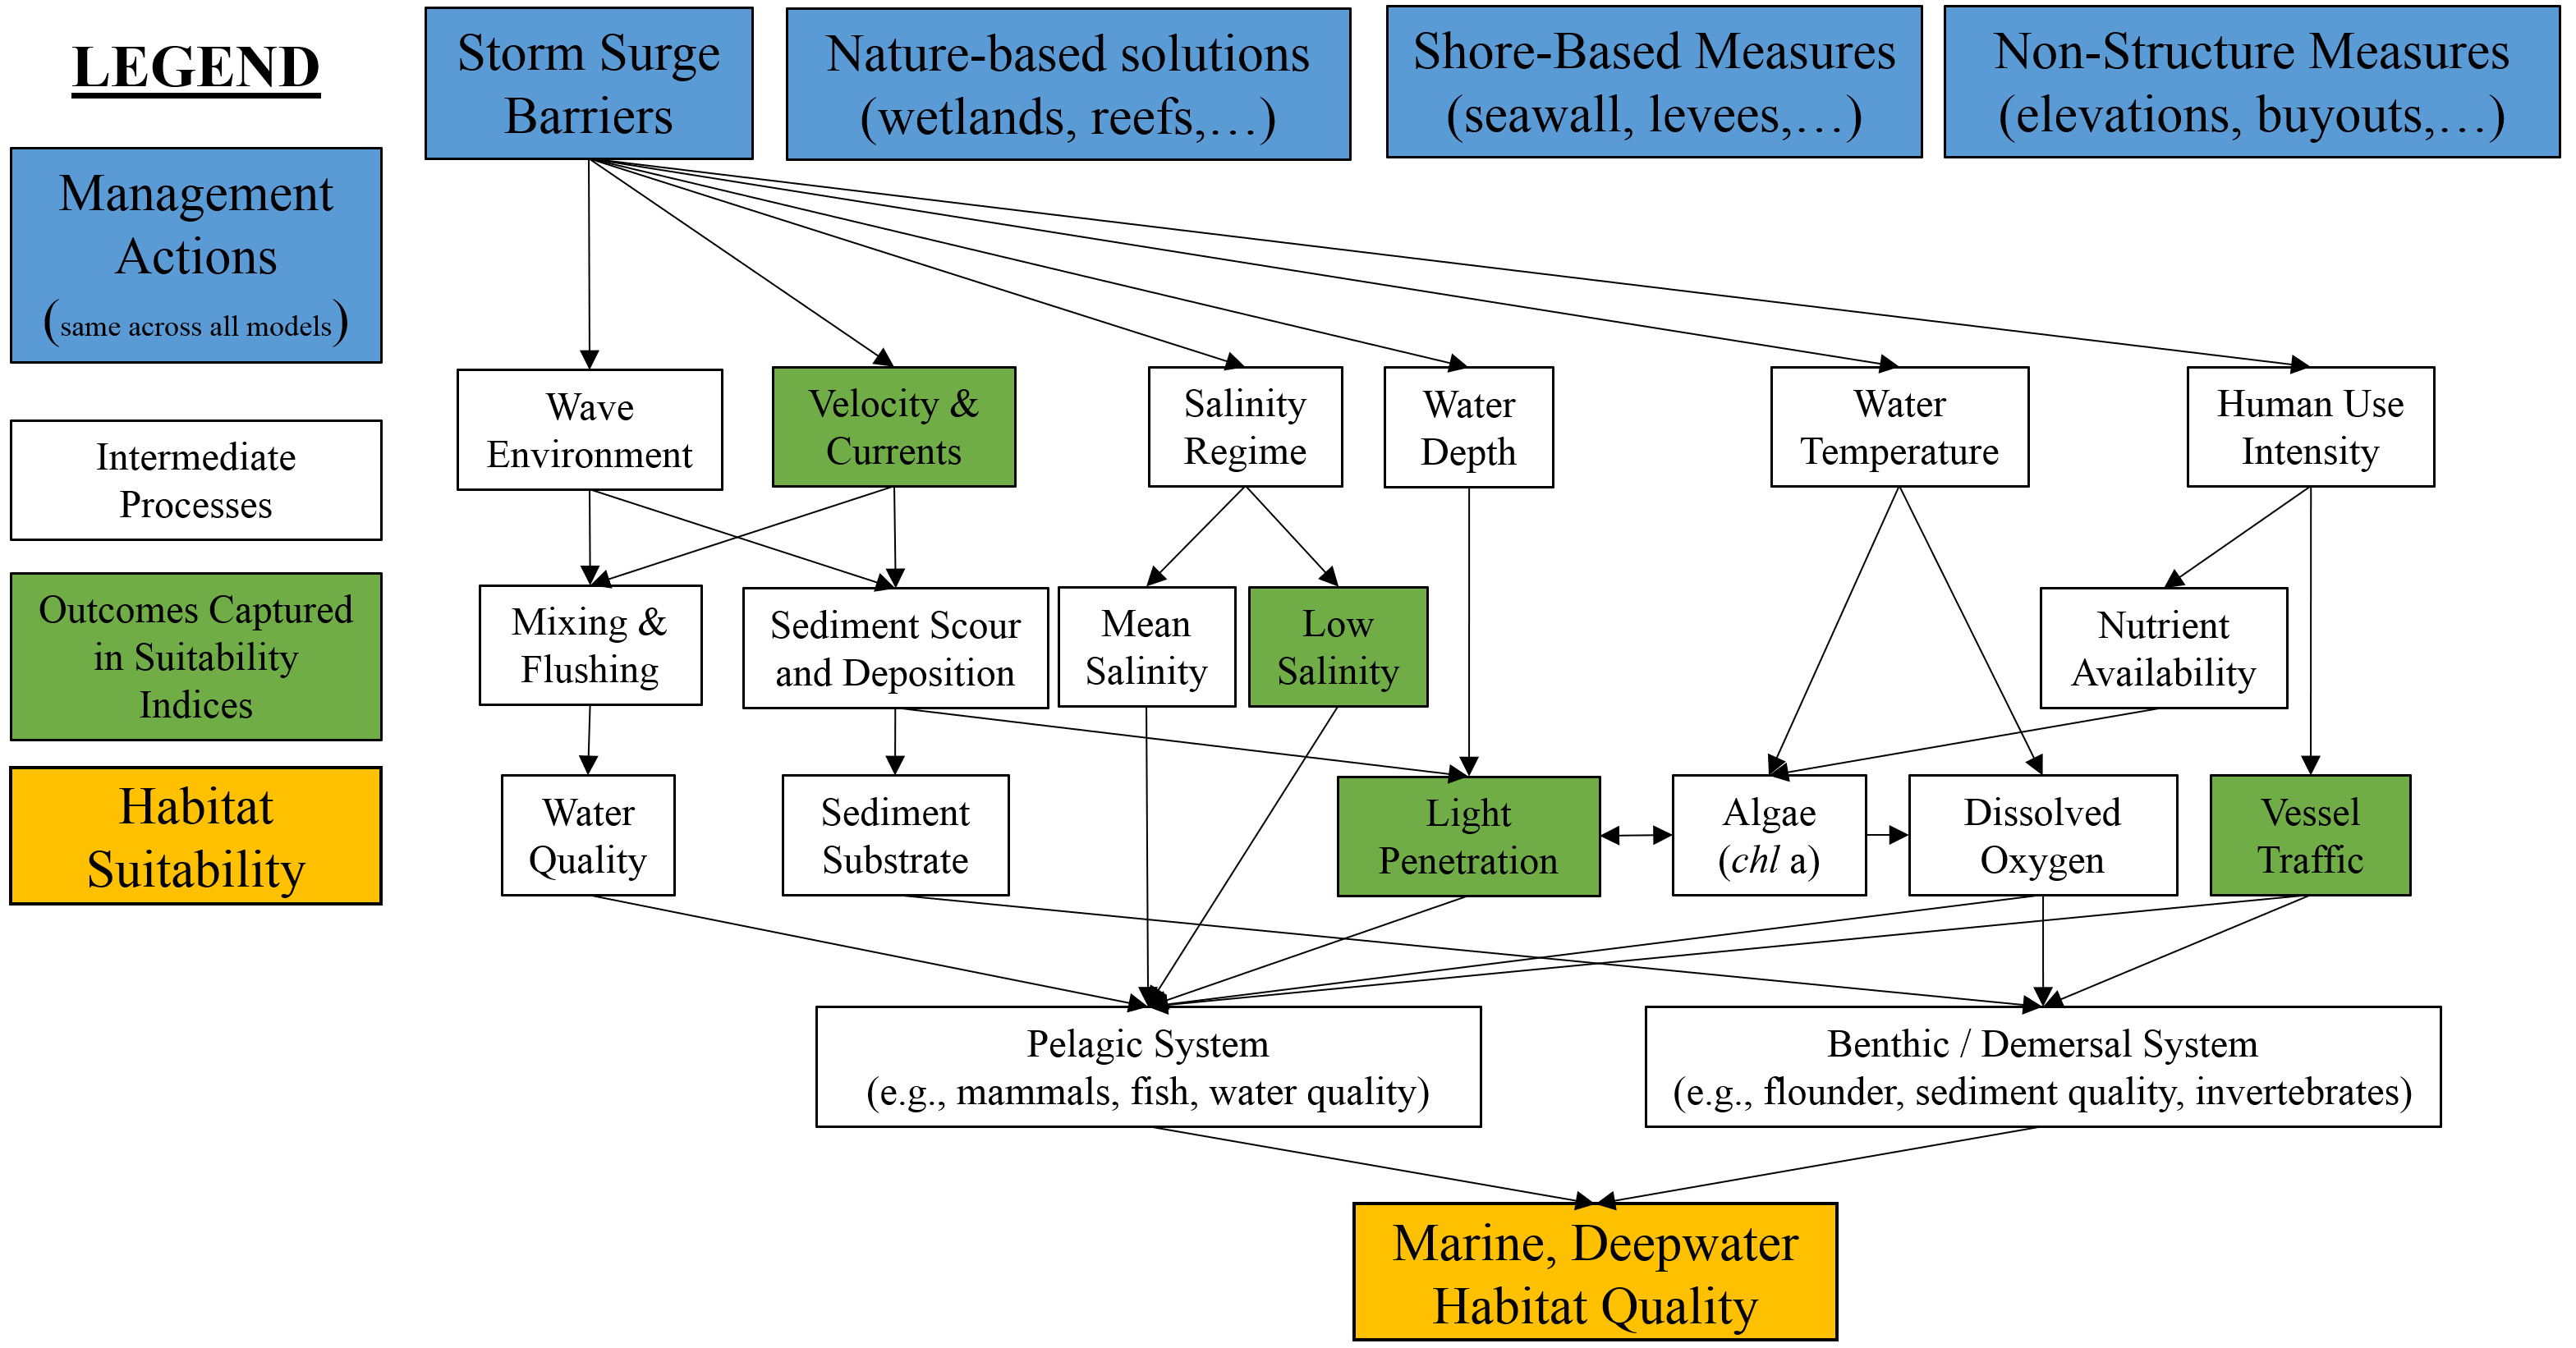
\includegraphics[width=43.57in]{ZZ_Fig04.14_Mar.Deep_ConModel} \caption{Conceptual model for the marine, deepwater submodel.}\label{fig:unnamed-chunk-23}
\end{figure}

The following variables are used to assess the marine deepwater submodel: a) salinity, b) velocity and currents, c) light attenuation, and d) vessel traffic. Salinity acts as a proxy for vertical mixing of the water column and influence of freshwater inputs \citep{smit_assessing_2021}. Current velocities represent mixing and flushing of the system, sediment suspension, and benthic scouring. Light penetration depths within the water column indicate water column turbidity, nutrient loading and algal production levels. Finally, vessel traffic provides an index for development pressures, both i) commercial and recreational fishing pressure on the pelagic, demersal and benthic systems, and ii) commercial and recreational vessel density pressures on the marine mammal populations within the area (population stress from ship strikes and noise pollution). The overall habitat suitability of the marine, deepwater zone may then be aggregated into a single metric via an arithmetic mean of suitability indices for these four metrics.

\(I_{mar.deep} = \frac{salinity.low.dur + velocity.low.change + light + vessel.density}{4}\)

Where \(I_{mar.deep}\) is an overarching index of ecosystem quality for the marine intertidal zone, \(salinity.low.dur\) is a suitability index relative to low salinity periods, \(velocity.low.change\) is a suitability index relative to changes in low velocity, \(light\) is a suitability index relative to light penetration through water, and \(vessel.density\) is a suitability index relative to ship traffic. All indices are quality metrics scaled from 0 to 1, where 0 is unsuitable and 1 is ideal.

\begin{figure}
\centering
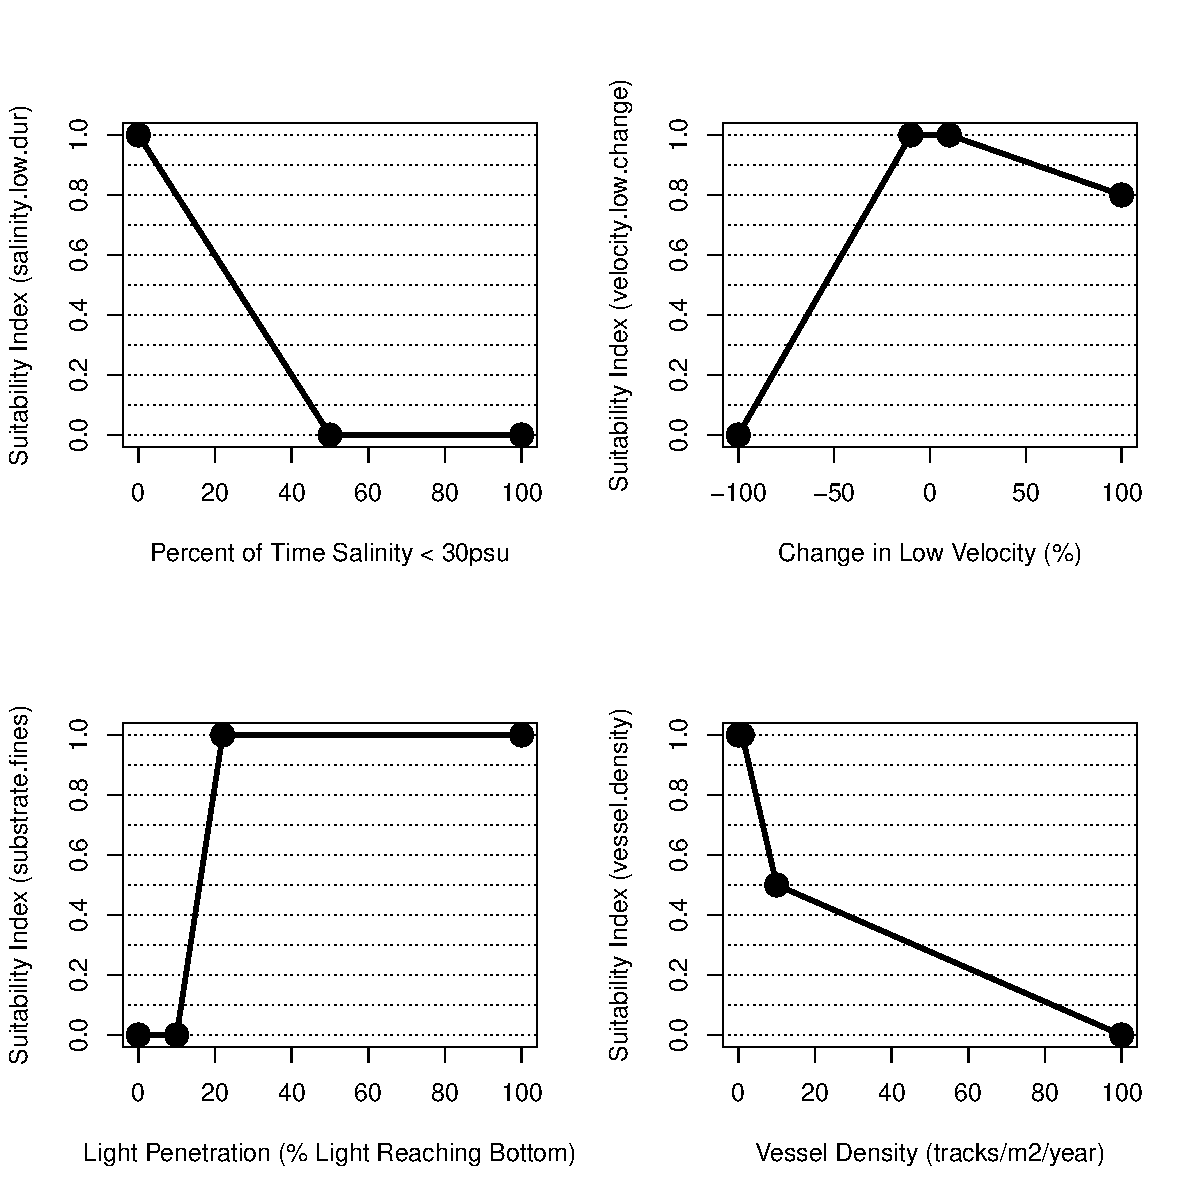
\includegraphics{_main_files/figure-latex/unnamed-chunk-24-1.pdf}
\caption{\label{fig:unnamed-chunk-24}Suitability index curves for the marine, deepwater zone.}
\end{figure}

\hypertarget{salinity-2}{%
\subsection{Salinity}\label{salinity-2}}

Salinity, often used as a proxy for the total concentration of all dissolved salts in the water, is a key factor in water density that controls the vertical mixing of nutrients and chemicals throughout the water column. Salinity constrains dissolved oxygen concentration and limits speciation of marine zones to euryhaline taxa that are physiological adapted to tolerate hypoosmotic processes (are able to maintain a lower internal ionic concentration than seawater).

For NYBEM, the salinity regime is summarized through a metric of the percent of time salinity is less than the marine ecosystem threshold of 30 psu. This approach assumes that freshwater inputs serve as disturbance on the ecosystem, and higher marine levels of salinity are preferred. Depth-averaged salinity is computed or measured at small time steps over and annual timeframe. These data may then be summarized as an ``exceedence curve'' with thresholds from 0-100\% in 10\% intervals. For NYBEM, this exceedence curve is used to calculate the percent of time salinity is less than or equal to 30 psu.

This duration metric is then translated into a suitability metric as follows:

\[salinity.low.dur = \begin{pmatrix} -0.02*sal_{dur}+1 & sal_{dur}=0-50\\
0.0 & sal_{dur}=50-100
\end{pmatrix}\]

Where \(salinity.low.dur\) is a suitability index relative to low salinity periods and \(sal_{dur}\) is the percent of time salinity is less than the threshold for marine habitat (i.e., salinity \textless{} 30 psu).

\hypertarget{current-velocity}{%
\subsection{Current Velocity}\label{current-velocity}}

The marine deepwater environment is subjected to velocity effects from ocean currents and tides that affect vertical and horizontal mixing and flushing of the system, suspended sediment and solids, substrate settlement of taxa, as well as the operation of small and recreational vessels. Low flow conditions allow for the settlement of sediment, possibly burying viable habitat, reducing mixing and flushing, and potentially facilitating hypoxic conditions. Conversely, high velocities scour the benthic environment, prohibiting settling in the substrate by benthic taxa.

Low flow conditions are particularly of concern for these processes, so a representative low velocity (i.e., 10\% exceedance probability) is used within NYBEM as a key indicator metric. Suitability is then calculated based on the change in this low velocity relative to a baseline condition. For NYBEM, the baseline condition is assessed as the existing condition for a representative tidal year. Suitability declines linearly beyond a 10\% change in this metric from the baseline with sharper decreases as velocities slow.

\[velocity.low.change = \begin{pmatrix} 0.011*vel_{rel}+1.11 & vel_{rel}=-100-10\\
1.0 & vel_{rel}=-10-10\\
-0.0022*vel_{rel}+1.02 & vel_{rel}>10
\end{pmatrix}\]

Where \(velocity.low.change\) is a suitability index relative to change in low velocity and mixing and \(vel_{rel}\) is the relative change in low velocity from a baseline condition assessed as:

\(vel_{rel}=\frac{vel_{10,f}-vel_{10,b}}{vel_{10,b}}\).

Where \(vel_{10,f}\) is the 10\% exceedence velocity for a focal condition and \(vel_{10,b}\) is a 10\% exceedence velocity for a baseline condition.

\hypertarget{light-1}{%
\subsection{Light}\label{light-1}}

The depth that light reaches within the water column acts as a proxy for the viability of water column turbidity, nutrient loading, and chlorophyll-a production (an essential building block for ocean productivity). As light controls chlorophyll-a production, it may be seen as a limiting factor for algal and particulate organic matter densities, and ultimately the development of harmful algal blooms. Therefore, light provides a meaningful metric for a variety of biological processes in this ecosystem. For the \texttt{mar.deepsub}, light availability and suitability are modeled following the same algorithms described for the \texttt{est.sub} model (See Section 4.4), which can be summarized in suitability terms as as:

\[light = \begin{pmatrix} 0.0 & PLA<10\\
0.0833*PLA-0.83 & PLA>70\\
1.0 & PLA>22\\
\end{pmatrix}\]

Where \(light\) is a suitability index relative to light penetration and \(PLA\) is percent light available (PLA).

\hypertarget{vessel-traffic}{%
\subsection{Vessel Traffic}\label{vessel-traffic}}

Vessel traffic density provides an index for development pressures, both commercial and recreational fishing pressure, and commercial and recreational vessel density pressures on the marine mammal populations within the area (population stress from ship strikes and noise pollution). Vessel use density from the historical Automatic Identification System (AIS) vessel data from the MARCOS portal are assessed within the NYBEM to identify the general use of waterways. These data also indicate frequently visited fishing locations and offshore structures. Suitability is computed for this metric analogously to \texttt{est.sub} and \texttt{mar.sub} algorithms as follows:

\[vessel.density = \begin{pmatrix} 1.0 & ves_{AIS}=0-1\\
-0.0556*ves_{AIS}+1.06 & ves_{AIS}=1-10\\
-0.00556*ves_{AIS}+0.56 & ves_{AIS}=10-100\\
0.0 & ves_{AIS}>100
\end{pmatrix}\]

Where \(vessel.density\) is a suitability index relative to ship traffic and \(slope_{per}\) is the slope of the beach perpendicular to the mean tide line in percent.

\hypertarget{potential-extension-of-marine-deepwater-model}{%
\subsection{Potential extension of marine, deepwater model}\label{potential-extension-of-marine-deepwater-model}}

The marine deepwater zone is affected by many processes not included in NYBEM. Future model development could explore the following:

\begin{itemize}
\tightlist
\item
  Dissolved oxygen concentration, a key element for the survival of marine species, limits speciation of marine zones through hypoxia, where low oxygen levels may cause die-offs in marine species. Dissolved oxygen concentrations act as a proxy for pelagic, demersal and benthic fauna biomass (abundance/diversity of phytoplankton, zooplankton, fish, marine turtles, birds and mammals). Data could potentially be integrated from sources such as permanent monitoring stations, as supported by NYC DEP Monitoring Stations (2018), Jamaica Bay Eutrophication Model \citep{fischbach_building_2018}, frameworks such as the Chesapeake Bay model \citep{cerco_threedimensional_1993}, and the EPA Long Island Sound integrated model (underway).\\
\item
  Water temperature acts as a control for the majority of the chemical (dissolved nutrients, pH, density, and photosynthesis), biological (respiration and metabolic rates, taxa development, and migrations) and physical (ice formation and thermal stratification of the water column) properties of a marine ecosystem. Methods could be adapted from the Winter flounder habitat suitability model \citep{banner_usfws_2001} and VIMS 2018 habitat suitability models and the USACE Harbor monitoring \citep{usace_essential_2013}, and data could potentially be extracted from MARACOOS Monthly Sea Surface Temperature via the MARCO Mid-Atlantic Ocean Data Portal or via hydrodynamic model outputs.\\
\item
  The wave environment affects many variables with the New York Bight: vertical and horizontal mixing and flushing of the physical and chemical properties of the water, suspended sediment and solids, substrate settlement of taxa, and commercial and recreational vessel traffic. Wave height and wave refraction could be assessed from analytical software such as STWAVE (\citet{byrnes_effects_2004}).\\
\item
  In the present iteration of NYBEM, light attenuation is assumed to be dependent on a single light coefficient (\(K_{d}\)). However, light attentuation can vary significantly based on suspended sediment concentration, algal processes, or water color, all of which may vary in time. Future version of the model could also consider spatially distributed data sets of light coefficients such as those by \href{https://www.fisheries.noaa.gov/inport/item/66148}{NOAA}.
\end{itemize}

\hypertarget{new-york-bight-overarching-model-nybem.wrapper-i}{%
\section{New York Bight Overarching Model (NYBEM.wrapper) (I)}\label{new-york-bight-overarching-model-nybem.wrapper-i}}

{Dougherty and McKay to write.}

\hypertarget{calculate-habitat-zones}{%
\subsection{Calculate habitat zones}\label{calculate-habitat-zones}}

\begin{Shaded}
\begin{Highlighting}[]
\CommentTok{\#Functions for isolating habitat types}

\DocumentationTok{\#\#\#\#\#\#\#\#\#\#}
\CommentTok{\#Labels for tidal zones}
\NormalTok{ZoneTidal }\OtherTok{\textless{}{-}} \FunctionTok{c}\NormalTok{(}\StringTok{"Deep"}\NormalTok{, }\StringTok{"Subtidal"}\NormalTok{, }\StringTok{"Intertidal"}\NormalTok{, }\StringTok{"Upland"}\NormalTok{)}

\CommentTok{\#Create function for isolating tidal zones}
\NormalTok{set.tidal.zone }\OtherTok{\textless{}{-}} \ControlFlowTok{function}\NormalTok{(bedelev, MLLW, MHHW)\{}
  \CommentTok{\#Assign zone}
\NormalTok{  tidalzone }\OtherTok{\textless{}{-}} \FunctionTok{ifelse}\NormalTok{(bedelev }\SpecialCharTok{\textless{}=} \SpecialCharTok{{-}}\DecValTok{2}\NormalTok{, }\DecValTok{1}\NormalTok{,}
          \FunctionTok{ifelse}\NormalTok{(bedelev }\SpecialCharTok{\textless{}=}\NormalTok{ MLLW, }\DecValTok{2}\NormalTok{,}
          \FunctionTok{ifelse}\NormalTok{(bedelev }\SpecialCharTok{\textless{}=}\NormalTok{ MHHW, }\DecValTok{3}\NormalTok{, }
          \FunctionTok{ifelse}\NormalTok{(bedelev }\SpecialCharTok{\textgreater{}}\NormalTok{ MHHW, }\DecValTok{4}\NormalTok{, }\ConstantTok{NA}\NormalTok{))))}
  \CommentTok{\#Send output}
\NormalTok{  tidalzone}
\NormalTok{\}}

\DocumentationTok{\#\#\#\#\#\#\#\#\#\#}
\CommentTok{\#Labels for salinity zones}
\NormalTok{ZoneSalinity }\OtherTok{\textless{}{-}} \FunctionTok{c}\NormalTok{(}\StringTok{"Marine"}\NormalTok{, }\StringTok{"Estuarine"}\NormalTok{, }\StringTok{"Fresh"}\NormalTok{)}

\CommentTok{\#Create function for isolating salinity zones}
\NormalTok{set.salinity.zone }\OtherTok{\textless{}{-}} \ControlFlowTok{function}\NormalTok{(salinity)\{}
  \CommentTok{\#Assign zone}
\NormalTok{  salinityzone }\OtherTok{\textless{}{-}} \FunctionTok{ifelse}\NormalTok{(salinity }\SpecialCharTok{\textgreater{}=}\DecValTok{30}\NormalTok{, }\DecValTok{1}\NormalTok{, }
                  \FunctionTok{ifelse}\NormalTok{(salinity }\SpecialCharTok{\textless{}} \DecValTok{30} \SpecialCharTok{\&}\NormalTok{ salinity }\SpecialCharTok{\textgreater{}=} \FloatTok{0.5}\NormalTok{, }\DecValTok{2}\NormalTok{, }
                  \FunctionTok{ifelse}\NormalTok{(salinity }\SpecialCharTok{\textless{}} \FloatTok{0.5} \SpecialCharTok{\&}\NormalTok{ salinity }\SpecialCharTok{\textgreater{}=} \DecValTok{0}\NormalTok{, }\DecValTok{3}\NormalTok{, }\ConstantTok{NA}\NormalTok{)))}
  \CommentTok{\#Send output}
\NormalTok{  salinityzone}
\NormalTok{\}}

\DocumentationTok{\#\#\#\#\#\#\#\#\#\#}
\CommentTok{\#Labels for habitat zones}
\NormalTok{ZoneHabitat }\OtherTok{\textless{}{-}} \FunctionTok{c}\NormalTok{(}\StringTok{"Upland"}\NormalTok{, }\StringTok{"Marine.Deep"}\NormalTok{, }\StringTok{"Marine.Subtidal"}\NormalTok{, }\StringTok{"Marine.Intertidal"}\NormalTok{, }\StringTok{"Estuarine.Subtidal"}\NormalTok{, }\StringTok{"Estuarine.Intertidal"}\NormalTok{, }\StringTok{"Freshwater"}\NormalTok{)}

\CommentTok{\#Create function for isolating habitat zones}
\NormalTok{set.habitat.zone }\OtherTok{\textless{}{-}} \ControlFlowTok{function}\NormalTok{(tidalzone, salinityzone)\{}
  \CommentTok{\#Assign zone}
\NormalTok{  habitatzone }\OtherTok{\textless{}{-}} \FunctionTok{ifelse}\NormalTok{(tidalzone }\SpecialCharTok{==} \DecValTok{4}\NormalTok{, }\DecValTok{1}\NormalTok{,}
          \FunctionTok{ifelse}\NormalTok{(salinityzone }\SpecialCharTok{==} \DecValTok{1} \SpecialCharTok{\&}\NormalTok{ tidalzone }\SpecialCharTok{==} \DecValTok{1}\NormalTok{, }\DecValTok{2}\NormalTok{,}
          \FunctionTok{ifelse}\NormalTok{(salinityzone }\SpecialCharTok{==} \DecValTok{1} \SpecialCharTok{\&}\NormalTok{ tidalzone }\SpecialCharTok{==} \DecValTok{2}\NormalTok{, }\DecValTok{3}\NormalTok{,}
          \FunctionTok{ifelse}\NormalTok{(salinityzone }\SpecialCharTok{==} \DecValTok{1} \SpecialCharTok{\&}\NormalTok{ tidalzone }\SpecialCharTok{==} \DecValTok{3}\NormalTok{, }\DecValTok{4}\NormalTok{,}
          \FunctionTok{ifelse}\NormalTok{(salinityzone }\SpecialCharTok{==} \DecValTok{2} \SpecialCharTok{\&}\NormalTok{ tidalzone }\SpecialCharTok{==} \DecValTok{1} \SpecialCharTok{|}\NormalTok{ tidalzone }\SpecialCharTok{==} \DecValTok{2}\NormalTok{, }\DecValTok{5}\NormalTok{,}
          \FunctionTok{ifelse}\NormalTok{(salinityzone }\SpecialCharTok{==} \DecValTok{2} \SpecialCharTok{\&}\NormalTok{ tidalzone }\SpecialCharTok{==} \DecValTok{3}\NormalTok{, }\DecValTok{6}\NormalTok{,}
          \FunctionTok{ifelse}\NormalTok{(salinityzone }\SpecialCharTok{==} \DecValTok{3} \SpecialCharTok{\&}\NormalTok{ tidalzone }\SpecialCharTok{==} \DecValTok{1} \SpecialCharTok{|}\NormalTok{ tidalzone }\SpecialCharTok{==} \DecValTok{2} \SpecialCharTok{|}\NormalTok{ tidalzone }\SpecialCharTok{==} \DecValTok{3}\NormalTok{, }\DecValTok{7}\NormalTok{, }\ConstantTok{NA}\NormalTok{)))))))}
  \CommentTok{\#Send output}
\NormalTok{  habitatzone}
\NormalTok{\}}
\end{Highlighting}
\end{Shaded}

\hypertarget{suitability-index-calculator-si.calc}{%
\subsection{\texorpdfstring{Suitability Index Calculator (\texttt{SI.calc})}{Suitability Index Calculator (SI.calc)}}\label{suitability-index-calculator-si.calc}}

Insert description here as needed.

\hypertarget{zone-specific-habitat-quality-functions}{%
\subsection{Zone-specific habitat quality functions}\label{zone-specific-habitat-quality-functions}}

Insert description here as needed.

\hypertarget{rasterize-habitat-patches}{%
\subsection{Rasterize Habitat Patches}\label{rasterize-habitat-patches}}

\textbf{Do we need to reference the spatial coordinate systems? Maybe the R function or package used?}

\texttt{patch.rasterizer}: This function rasterizes the output of \texttt{patch.mapper} based on a specified grid resolution and aligns that layer with a specified spatial coordinate system.

\begin{Shaded}
\begin{Highlighting}[]
\CommentTok{\#Functions for rasterizing habitat types}
\NormalTok{patch.rasterizer }\OtherTok{\textless{}{-}} \ControlFlowTok{function}\NormalTok{(patch.mapper.output, grid.resolution, my.coordinate.system)\{}
  \CommentTok{\#Insert code}
\NormalTok{\}}
\end{Highlighting}
\end{Shaded}

\hypertarget{other-fxns-as-needed}{%
\subsection{Other fxns as needed}\label{other-fxns-as-needed}}

Numerical code for running the entire model suite

\begin{Shaded}
\begin{Highlighting}[]
\CommentTok{\#Function }
\NormalTok{NYBEM.wrapper }\OtherTok{\textless{}{-}} \ControlFlowTok{function}\NormalTok{(x, y)\{}
\NormalTok{  NYBEM.out }\OtherTok{\textless{}{-}}\NormalTok{ x }\SpecialCharTok{+}\NormalTok{ y}

  \CommentTok{\#Send output}
\NormalTok{  NYBEM.out}
\NormalTok{\}}
\end{Highlighting}
\end{Shaded}

\hypertarget{evaluation-i}{%
\chapter{Evaluation (I)}\label{evaluation-i}}

{McKay will complete by April 1.}

Ecological models such as NYBEM, typically rely on multiple variables, ecological processes, and in many cases present a variety of ecological outcomes. As such, models can quickly become complex system representations with many components, inputs, assumptions, and modules. Model evaluation is the process for ensuring that numerical tools are scientifically defensible and transparently developed. Evaluation is often referred to as verification or validation, but it in fact includes a family of methods ranging from peer review to model testing to error checking (Schmolke et al.~2010). In this more general sense, evaluation should include the following \citep{grant_ecological_2008}: (1) assessing the reasonableness of model structure, (2) assessing functional relationships and verifying code, (3) evaluating model behavior relative to expected patterns, (4) comparing outcomes to empirical data, if possible, and (5) analyzing uncertainty in predictions. The USACE has established an ecological model certification process to ensure that planning models are sound and functional. These generally consist of evaluating tools relative to the three following categories: system quality, technical quality, and usability (EC 1105-2-412).

\hypertarget{system-quality}{%
\section{System Quality}\label{system-quality}}

Ecological models must not only maintain an appropriate theoretical and technical basis, but also must be computationally accurate (McKay et al.~2021b). System quality refers to the computational integrity of a model (or modeling system). For instance, is the tool appropriately programmed, has it been verified or stress-tested, and do outcomes behave in expected ways? NYBEM's system quality was evaluated in a variety of ways, including the following:

\begin{itemize}
\item
  \emph{Code checking:} All code was error-checked during development by the primary programmer, and team members and interagency partners will be encouraged to inspect models as well. To date, quality assurance activities have included consistent variable naming, investigation of outputs from each individual line of code, and blocks of code (e.g., functions and loops).
\item
  \emph{Function Testing:} Spatial zonation functions were tested with 100 randomized input sets of salinity, bed elevation, MHHW, and MLLW (Table 4). All outputs produced the anticipated outcomes based on manual inspection of the data. \textbf{ADD description of package testing with testthat.}
\end{itemize}

\hypertarget{technical-quality}{%
\section{Technical Quality}\label{technical-quality}}

The NYBEM includes a number of parameters that have long been recognized as crucial to the health of coastal ecosystems. Model assessments were used or adapted from existing peer-reviewed models whenever possible (e.g., \citep{usace_evaluation_2009}, plover (\citep{farmer_habitat_2000}, \citep{seavey_effect_2011}), horseshoe crab (\citep{avissar_modeling_2006}, \citep{nancy_jackson_armoring_2010}, \citep{lathrope_mapping_2013}, \citep{brady_habitat_1996}), amaranth \citep{sellars_habitat_2007}, sea turtles \citep{dunkin_spatially_2016}).
Suitability curves and associated inputs, on the other hand, rely substantially on expert judgment and postulated coastal ecosystem functions. These methods have been found to have great utility and predictive value, and they are still widely utilized in ecological assessments (Hughes et al.~2010).

\begin{itemize}
\tightlist
\item
  Interagency workshops (Appendix A) for informal input and review.
\end{itemize}

As a tool to examine the ecological impacts of infrastructure alternatives in a large, diversified ecosystem, the NYBEM is coupled to hydrodynamic model outcomes. This is a significant distinction between SLAMM and other long-term forecasting models. The inclusion of hydrodynamic model results is intended to quantify key physical processes within the ecosystem, with the model capable of influencing engineering design and assessing environmental impact. This model was used to create baseline conditions across the whole study area, and then construct habitat suitability curves to assess the potential impacts.

The technical quality of a model is assessed relative to its reliance on contemporary theory, consistency with design objectives, and degree of documentation and testing. NYBEM is being developed with a variety of ecological modeling methods for analyzing coastal ecosystems. The patch-scale quantity/quality framework has been applied extensively to assess outcomes ranging from the species to ecosystem levels of hierarchy (e.g., habitat evaluation procedures and the hydrogeomorphic methods, respectively). Furthermore, each sub-model is being developed with existing models and supported by peer reviewed methods developed elsewhere. System-scale connectivity models will do the same as well. To date, technical quality has been informally assessed through multiple development workshops.

\textbf{Future evaluations of technical quality will include:}

\begin{itemize}
\item
  Habitat zones will be compared to existing condition habitat maps through the National Wetlands Inventory and analogous state data sets (e.g., submerged aquatic vegetation and shellfish data sets).
\item
  Informal review of model structure will continue with the interagency partners involved in development to date.
\item
  Sensitivity analyses will be conducted to evaluate the relative importance of variables.
\end{itemize}

\hypertarget{usability}{%
\section{Usability}\label{usability}}

The usability of a model can influence the repeatable and transparent application of a tool. This type of evaluation typically examines the ease of use, availability of inputs, transparency, error potential, and education of the user. As such, defining the intended user(s) is a crucial component of assessing usability. The NYBEM was developed for application by the USACE technical team of the NJBB and HATS studies. The tool is not currently intended for broader application by local sponsors, other regional teams, or by other USACE Districts. As such, there is currently no graphical user interface for the model beyond the script itself. To date, the primary mechanism for maintaining usability is development in Rmarkdown which allows for transparent sharing of code within model documentation.
No graphic user interface (GUI) right now, but other methods were used to increase useability. Main talking points

\begin{itemize}
\tightlist
\item
  Reproducible research methods.
\end{itemize}

For a substantial and growing proportion of research experts developing novel statistical algorithms, R is the primary language. CRAN (Comprehensive R Archive Network) makes it simple to learn from others' work, share your own, and receive comments on possible changes. Packaging the NYBEM improves usability by providing a system for developing software that includes documentation and tests, resulting in higher software quality and development productivity.

Version control helps to maintain track of work and review the changes made to the NYBEM, whether they're to data, coding scripts, or notes. Version control is considerably smoother and easier to apply with version control software like Git. Furthermore, storing the NYBEM on the online platform Github creates an online backup, which is helpful to all contributors.

\begin{itemize}
\tightlist
\item
  Open source national and regional data sets and publishing of AdH outcomes.
\end{itemize}

Utilizing previously-published high-value data sets in the NYBEM can increase transparency and accountability to the public and stakeholders.

\textbf{Future evaluations of usability will include:}

\begin{itemize}
\item
  Open data sharing of all site-specific inputs and outputs for interrogation by internal and external partners.
\item
  Training of project team members on the use of NYBEM.
\item
  Archival and sharing of code with the ERDC ecological modeling team and the USACE Ecosystem Restoration Planning Center of Expertise.
\end{itemize}

\hypertarget{application-and-communication}{%
\chapter{Application and Communication}\label{application-and-communication}}

The NYBEM has been explicitly designed to inform site screening and environmental impact assessment for the NJBB and HATS. A key component of this process is understanding the existing condition without project effects. This section presents a preliminary application of the NYBEM to assess ecosystem condition in the New Jersey Back Bays following four main activities:

\begin{itemize}
\tightlist
\item
  Incorporation of hydrodynamic model outcomes,\\
\item
  Compilation of other environmental input data sets for the NYBEM in this region,\\
\item
  Execution of the models, and\\
\item
  Summary of model outcomes.
\end{itemize}

\hypertarget{njbb-hydrodynamic-modeling}{%
\section{NJBB Hydrodynamic Modeling}\label{njbb-hydrodynamic-modeling}}

Adaptive Hydraulics (AdH) is the numerical model code applied for hydrodynamic simulations in this study. For this study, the two-dimensional (2D) shallow water module of AdH is applied for all simulations. This code solves for depth-averaged velocity and salinity throughout the model domain. (More details of the 2D shallow water module of AdH and its computational philosophy and equations are available in Savant et al.~2014 and Savant and Berger 2015.) AdH version 4.6 was applied for this study.

A 2D AdH model was developed and validated for simulation of hydrodynamics and salinity (Details provided in McAlpin and Ross, \emph{draft}). The model was validated to available field data for all parameters and then utilized to test project alternatives for present and future sea level rise conditions. A field data collection effort was performed in February 2019 to collect salinity and discharge/velocity data over a 13-hour tidal cycle at three major inlets -- Barnegat, Little Egg, and Great Egg. Field data supported the use of a 2D model as opposed to a three-dimensional (3D) model due to lack of major salinity stratification.

The model domain was determined using aerial images and bathymetry/topographic data for the area. The Surface Water Modeling System was used to generate a 2D surface mesh and define material regions for applying specific model features, such as bed roughness. The domain is defined horizontally in Universal Transverse Mercator, zone 18 coordinates with units of meters. Vertically it is based on North American Vertical Datum of 1988 (NAVD88) with units of meters. All data applied to the model are shifted to this datum and coordinate system. Bathymetry data for the model were obtained from several sources: the Coastal Relief Model, sponsor collected hydrographic surveys, and the National Elevation Dataset. These data sets were combined such that the latest data were made a priority as well as data collected at finer resolution. The 2D AdH code can include areas that wet/dry; therefore, elevations were included in the domain up to 2 m NAVD88.

The model domain includes over 9,867 square miles, extending approximately 115 miles along the New Jersey Atlantic Ocean coastline from Lewes, DE, to Manasquan, NJ. The 2D mesh contains 324,881 elements and 165,514 nodes. Figure 6.1 shows horizontal node resolution for the model with an example region surrounding the Barnegat Bay Inlet. Resolution is finest in the small wetland channels to accurately capture the conveyance of flow in these areas as well as the salinity that migrates upstream in deeper channels. Finer resolution is also seen in areas where geometric features need to be defined accurately, such as in the inlets and around jetties.

{INSERT FIGURE 6.1}

Ten AdH simulations were executed: seven project alternatives and three projects rerun with sea level change. An elevation shift of 0.445 m was added to the water surface elevation at the tide boundary for sea level rise simulations to reflect the ``intermediate'' sea level rise curve in the year 2080 (per EC 1165-2-212). The mesh domain was not expanded to account for potential wetted area with rising sea level. Additionally, vegetated areas were not raised in the sea level rise simulations. Only the existing condition scenario is presented here.

AdH was executed for a ``base'' condition representing 2018, which is assumed here to be the ``future without project'' (FWOP) condition from a project planning perspective. For all simulations, outputs included the following:

\begin{itemize}
\tightlist
\item
  Water surface elevations (MHHW and MLLW)\\
\item
  Salinity levels (mean)\\
\item
  Velocity
\end{itemize}

Bed elevation, water surface elevation (MHHW and MLLW), and salinity were input to the zonation functions shown in the Quantification section of this report. Figure 6.2 shows representative outputs from these functions for salinity and tidal zones as well as habitat types in the Barnegat Bay Inlet and Absecon Inlet. Notably, these habitat zones represent only AdH outputs and do not necessarily reflect regulatory definitions of ecosystems. For instance, an area identified as an estuarine, subtidal ecosystem may (or may not) currently host submerged aquatic vegetation or hard-bottom reef environments, which would imply very different outcomes from a management perspective. Likewise, an estuarine, intertidal zone may currently be developed and non-functional from an ecological perspective. However, these outputs provide broad spatial coverage not feasible to collect for the entire study area.

{INSERT FIGURE 6.2}

\hypertarget{environmental-data-compilation}{%
\section{Environmental Data Compilation}\label{environmental-data-compilation}}

Insert.

\hypertarget{model-execution}{%
\section{Model Execution}\label{model-execution}}

Insert text describing the rasterization of data sets and any numerical magic.

\hypertarget{summary-of-nybem-outcomes}{%
\section{Summary of NYBEM Outcomes}\label{summary-of-nybem-outcomes}}

Insert.

\hypertarget{summary}{%
\chapter{Summary}\label{summary}}

This report has presented the development status for the New York Bight Ecological Model (NYBEM). The models are being developed in a transparent manner following a mediated modeling process (Herman et al.~2019). The phased development of these models is designed to incorporate information and data as they are developed. The models have been applied in the context of the New Jersey Back Bays (NJBB) coastal storm risk management study, and some preliminary observations are made regarding the relative effects of alternatives (Section 6 of this report).
As of this writing, the NYBEM only assesses habitat quantity, although future development will expand this scope. The following items represent key priorities for additional expansion of both the model and its application.

\begin{itemize}
\item
  Habitat quality modules should be incorporated based on the workshop-based suitability index curves.
\item
  The system-wide connectivity model can be developed and executed, potentially to include multiple organisms or groups of organisms.
\item
  The models should be submitted and reviewed through the USACE Model Certification process.
\item
  Additional model evaluation should occur, including issues such as: verification of habitat assessment relative to field observations and sensitivity analysis of the underlying model structure.
\item
  Applications should be expanded to incorporate more tidal years (including storm periods), alternative operational closure scenarios, more sea level rise conditions, and other project-relevant factors.
\end{itemize}

\hypertarget{future-model-development}{%
\section{Future Model Development}\label{future-model-development}}

Currently, only habitat quantity is included in assessments. Model development is underway relative to habitat quality modules, system connectivity, and aggregation of quantity, quality, and connectivity into an overarching environmental effects index. These assessments will be included in the NJBB Final Feasibility Report.

\emph{Undeveloped Areas}: USACE projects are required to account and mitigate for detrimental environmental effects associated with any recommended actions. However, the region is highly developed, and USACE should not be penalized for existing ecological impacts. As such, developed areas are removed from the domain as these represent impacts not attributable to USACE projects. Developed areas were assessed via the 2016 National Land Cover Dataset (NLCD) as open space, low intensity, medium intensity, and high intensity classes (Codes 21, 22, 23, and 24). The reduced model domain is 1,720 mi\textsuperscript{2}, which includes all areas potentially assessed for impacts.

\hypertarget{habitat-quality-modules}{%
\subsection{Habitat Quality Modules}\label{habitat-quality-modules}}

Ecosystem quality may be differentially assessed for each of the six habitat types shown in Table 3, which we refer to as sub-models or modules. An index-based model is being developed for each ecosystem based on existing data and models. A consistent set of methods was used to develop each sub-model. First, candidate variables were identified at workshops and augemented with taxa-specific habitat suitability models (i.e., ``blue books''), relevant tools (e.g., New England Marsh Model), and literature search. Second, system-wide data sets were compiled from national data layers, hydrodynamic models, and other data sources (e.g., Mid-Atlantic Ocean Data Portal, \href{https://portal.midatlanticocean.org/}{MARCO}). Third, potential variables were compiled and rationale was developed supporting the inclusion or exclusion of each. Fourth, an ecosystem-specific conceptual model was compiled to highlight key variables used in numerical model development. Fifth, ``suitability'' curves were developed for each variable based on existing suitability indices (e.g., from USFWS habitat models), published ecological thresholds/responses, and professional judgment / qualitative responses. These suitability curves represent the relative quality of a given patch on a 0 to 1 scale, where 0 is poor and 1 is ideal. Sixth, all suitability curves are arithmetically averaged to obtain an overall metric of ecosystem quality. Finally, all sub-models were vetted with interagency partners at a November 2019 workshop and refined accordingly.

For example, Figures 4 and 5 present a general summary of the development of the estuarine, subtidal sub-model. Key references and existing tools are noted along with transient or construction impacts and critical uncertainties. An ecosystem-specific conceptual model is presented. Potential variables are compiled along with specific metrics, assessment methods, and rationale for inclusion or exclusion in NYBEM. Finally, suitability curves are presented for this sub-model (Figure 5). Each sub-model will be presented in a similar detailed format prior to application. All index-based model calculations will be conducted with the \texttt{ecorest} R-package (McKay and Hernandez-Abrams 2020). \href{https://cran.r-project.org/web/packages/ecorest/index.html}{\texttt{ecorest}} is a generic software for conducting suitability index calculations, which will be submitted for USACE National Certification in Summer 2021.

\hypertarget{system-scale-connectivity-model}{%
\subsection{System-Scale, Connectivity Model}\label{system-scale-connectivity-model}}

The index models described above focus on patch-scale outcomes in each of the six nearshore and estuarine ecosystem types, and a broader connectivity model will also be developed to assess outcomes at a system-scale. This analysis will focus on relative changes in hydrologic connectivity between ecosystems, which is defined as the ``water-mediated transfer of matter, energy, and/or organisms within or between elements of the hydrologic cycle'' (Pringle 2001). For the purpose of NYBEM, we will focus on connectivity relative to organismal outcomes; for instance, closure gates and storm surge barriers have the potential to disrupt animal movement between different habitat patches required during an organism's life cycle. An analytical approach has not been finalized, but analogous freshwater connectivity models have included issues such as the quantity and quality of habitat patches scaled by movement rates around structures (McKay et al.~2017). For instance, the ``passability'' of a structure could be used to scale the total amount of upstream habitat for a migratory fish such as river herring. These methods could potentially be adapted for multi-directional movement in the context of estuarine connectivity.

\hypertarget{aggregated-model-outcomes}{%
\subsection{Aggregated Model Outcomes}\label{aggregated-model-outcomes}}

Model outcomes from both the patch- and system-scales will need to be aggregated into a small number of summary metrics for USACE decision-makers. All ecological outcomes will estimated at discrete points in time (e.g., 2030, 2080), and a time-averaged assessment of ecological condition (i.e., an ``annualized'' outcome) will provide a consistent means of comparing alternatives over long planning horizons (e.g., 50-years). Furthermore, a given ecosystem type may decline under sea level rise without an agency action, and proposed alternatives should be considered relative to background rates of change.

\hypertarget{appendix-appendices}{%
\appendix}


\hypertarget{model-development-workshops}{%
\chapter{Model Development Workshops}\label{model-development-workshops}}

NYBEM has been developed through a series of workshops with USACE and non-USACE partners. This appendix provides a brief overview of workshop details.

\textbf{January 3, 2019}

\emph{Location}: USACE Philadelphia District

\emph{Attendees}:

\begin{itemize}
\tightlist
\item
  USACE-NAP Planning: Steve Allen, Scott Sanderson, Regina Kukola\\
\item
  USACE-NAP Engineering: Laura Bittner, Sam Weintraub, Rob Hampson, Mary Pakan\\
\item
  USACE-ERDC: Kyle McKay
\end{itemize}

\emph{General scope and key outcomes}:

\begin{itemize}
\tightlist
\item
  General overview of ecological model development\\
\item
  Preliminary conceptual model development with identification of model components\\
\item
  General categorization of conceptual model components and preliminary rendering
\end{itemize}

\textbf{March 11, 2019}

\emph{Location}: USACE New York District

\emph{Attendees}:

\begin{itemize}
\tightlist
\item
  USACE-NAP: Steve Allen, Rob Hampson\\
\item
  USACE-NAN: Jesse Miller, Daria Mazey, Peter Weppler, Seika Robinson, Ryan Corbett, Olivia Cackler, Bryce Wisemiller\\
\item
  USACE-NAB: Angie Sowers\\
\item
  USACE-ERDC: Kyle McKay, Todd Swannack, Darixa Hernandez-Abrams\\
\item
  U.S. Environmental Protection Agency: Barbara Spinweber (by phone)
\end{itemize}

\emph{General scope and key outcomes}:

\begin{itemize}
\tightlist
\item
  Presentation of the preliminary conceptual model from the January 2019 meeting.\\
\item
  Discussion of key ecological outcomes that need to be addressed (e.g., listed species).\\
\item
  A habitat-type modeling approach was proposed to reduce the dimensionality and complexity of the modeling problem. Three overarching systems were identified as potential framing for model development: (1) marine / oceanside systems, (2) estuarine / bayside systems, and (3) network connectivity for the entire ecosystem.\\
\item
  For each habitat type the following issues were identified: key sub-types of habitats, construction impacts, operational impacts, direct effects (e.g., footprint effects) vs.~indirect effects (e.g., changes in circulation), key intermediate processes that a model would need to capture, and key data / modeling resources.\\
\item
  A key action item was organization of a broader workshop with other agencies, entities, and project sponsors in early summer.
\end{itemize}

\textbf{June 6, 2019}

\emph{Location}: 290 Broadway, New York

\emph{Attendees}:

\begin{itemize}
\tightlist
\item
  USACE-NAP: Steve Allen, Laura Bittner, Rob Hampson, J.B. Smith\\
\item
  USACE-NAN: Olivia Cackler, Arun Heer, Dag Madara, Daria Mazey, Jesse Miller, Carissa Scarpa, Peter Weppler, Bryce Wisemiller\\
\item
  USACE-ERDC: Anthony Emiren, Darixa Hernandez-Abrams, Tate McAlpin, Kyle McKay\\
\item
  U.S. Fish and Wildlife Service: Kerri Dikun, Steve Mars\\
\item
  National Oceanic and Atmospheric Administration: Karen Greene\\
\item
  National Park Service: Amanda Babson, Catherine Johnson, Patricia Rafferty\\
\item
  U.S. Environmental Protection Agency: Lingaard Knutson, Mike Poetzsch, Barbara Spinweber\\
\item
  U.S. Coastal Guard: Jeff Yunker\\
\item
  U.S. Geological Survey: Stephen Terrancino\\
\item
  New Jersey Department of Environmental Protection: Kelly Davis, Vanessa Domish, Colleen Keller, Shanna Madsen, Kunal Patel, Clay Sherman, Alexis Taylor, Rob Von Briel\\
\item
  New York State Department of State: Terra Haight\\
\item
  New York State Department of Environmental Conservation: Ryan Hodgetts
\item
  New York City Parks: Novem Auyeung, Mitchel Loring, Rebecca Swarke\\
\item
  New York City Department of Environmental Protection: Nusrat Begum, Andrew Chao, Megan Furrelle, Rupal Mehta\\
\item
  New York City Mayor's Office of Resiliency: Cherry Mui\\
\item
  Barnegat Bay Partnership: Stan Hales, Jim Vasslides\\
\item
  Hudson River Foundation: Jim Lodge\\
\item
  Stevens Institue: Philip Orton
\end{itemize}

\emph{General scope and key outcomes}:

\begin{itemize}
\tightlist
\item
  Overview presentation on development approach for the New York Bight Ecological Model (NYBEM) by Dr.~Kyle McKay.\\
\item
  General feedback on the scope and overall approach.\\
\item
  The workshop centered on collection of notes and ideas via a series of posters devoted to each of eight ecosystem-specific models. Morning sessions emphasized identification of key variables and processes, and afternoon sessions developed preliminary conceptual models of each ecosystem type along with qualitative responses in the form of habitat suitability curves.\\
\item
  Additional information was collection on key references, available data, existing models, and key expertise.
\end{itemize}

\textbf{November 14, 2019}

\emph{Location}: USACE New York District

\emph{Attendees}:

\begin{itemize}
\tightlist
\item
  USACE-NAP: Steve Allen\\
\item
  USACE-NAN: Cheryl Alkemeyer, Olivia Cackler, Jesse Miller, Alexandra Ryan, Carissa Scarpa, Danielle Tommaso, Peter Weppler, Bryce Wisemiller\\
\item
  USACE-ERDC: Kyle McKay, Darixa Hernandez-Abrams (phone)\\
\item
  U.S. Fish and Wildlife Service: Kerri Dikun (phone), Steve Papa (phone)\\
\item
  National Park Service: Patricia Rafferty\\
\item
  U.S. Environmental Protection Agency: Lingaard Knutson, Lance Caldwell, John Dawson\\
\item
  U.S. Coastal Guard: Jeff Yunker\\
\item
  U.S. Geological Survey: Liv Herdman, Chris Schubert\\
\item
  New Jersey Department of Environmental Protection: Christina Davis (phone), Kelly Davis (phone), Clay Sherman, Kelley Staffieri, Rob von Briel\\
\item
  New York State Department of Environmental Conservation: Joanna Field, Ryan Hodgetts
\item
  New York City Parks: Georgina Cullman, Marit Larsen\\
\item
  New York City Mayor's Office of Resiliency: Adam Parris\\
\item
  Hudson River Foundation: Rob Pirani\\
\item
  HDR: Chris Coccaro
\end{itemize}

\emph{General scope and key outcomes}:

\begin{itemize}
\tightlist
\item
  Overview of NYBEM development status and key open questions for discussion (Dr.~Kyle McKay)\\
\item
  General discussion of key overarching issues\\
\item
  Presentation of eight ecosystem-specific conceptual models based on prior workshops\\
\item
  Attendees refined, edited, and modified ecosystem-specific models
\end{itemize}

\hypertarget{model-testing}{%
\chapter{Model Testing}\label{model-testing}}

{Insert all of the testthat outcomes from Dougherty's package building.}

\hypertarget{hsiarimean}{%
\section{HSIarimean}\label{hsiarimean}}

\begin{table}

\caption{\label{tab:unnamed-chunk-29}Tests run on HSIarimean.}
\centering
\begin{tabular}[t]{c|c|c|c|c}
\hline
Target & In1 & In2 & In3 & In4\\
\hline
1.00 & 1 & 1 & 1 & 1\\
\hline
0.75 & 1 & 1 & 1 & 0\\
\hline
0.50 & 1 & 1 & 0 & 0\\
\hline
0.25 & 1 & 0 & 0 & 0\\
\hline
0.00 & 0 & 0 & 0 & 0\\
\hline
\end{tabular}
\end{table}

\begin{verbatim}
## Test passed
\end{verbatim}

\hypertarget{hsigeomean}{%
\section{HSIgeomean}\label{hsigeomean}}

\begin{table}

\caption{\label{tab:unnamed-chunk-30}Tests run on HSIgeomean.}
\centering
\begin{tabular}[t]{c|c|c|c|c}
\hline
Target & In1 & In2 & In3 & In4\\
\hline
1 & 1 & 1 & 1 & 1\\
\hline
0 & 1 & 1 & 1 & 0\\
\hline
0 & 1 & 1 & 0 & 0\\
\hline
0 & 1 & 0 & 0 & 0\\
\hline
0 & 0 & 0 & 0 & 0\\
\hline
\end{tabular}
\end{table}

\begin{verbatim}
## Test passed
\end{verbatim}

\hypertarget{usace-model-certification-review}{%
\chapter{USACE Model Certification Review}\label{usace-model-certification-review}}

Ecological models typically rely on multiple variables, ecological processes, and in many cases present a variety of ecological outcomes. As such, models can quickly become complex system representations with many components, inputs, assumptions, and modules. Model evaluation is the process for ensuring that numerical tools are scientifically defensible and transparently developed. Evaluation is often referred to as verification or validation, but it in fact includes a family of methods ranging from peer review to model testing to error checking (Schmolke et al.~2010). The USACE has established an ecological model certification process to ensure that planning models are sound and functional. These generally consist of evaluating tools relative to the three following categories: system quality, technical quality, and usability (EC 1105-2-412).

The NYBEM underwent USACE review and certification from March through April 2022. Models were reviewd by Larry Oliver (USACE New England District, ``Reviewer-1''), Dr.~Kelly Burks-Copes (USACE Galveston District, ``Reviewer-2''), Nate Richards (USACE Headquarters, ``Reviewer-3''), and Alicia Logalbo (USACE Norfolk District, ``Reviewer-4''). All comments follow the four-part comment structure of: (1) identify the problem, (2) describe the technical basis for the comment, (3) rate the significance or impact of the problem, and (4) recommend a mechanism for resolution. Comments and author responses are provided for transparency in review processes and long-term archival.

\textbf{Reviewer-1}

\emph{Comment 1.1: Insert.}

\begin{itemize}
\tightlist
\item
  \emph{Basis}: Insert.\\
\item
  \emph{Significance}: Insert.\\
\item
  \emph{Resolution}: Insert.\\
\item
  \emph{Author Response}: Insert.
\end{itemize}

\emph{Comment 1.2: Insert.}

\begin{itemize}
\tightlist
\item
  \emph{Basis}: Insert.\\
\item
  \emph{Significance}: Insert.\\
\item
  \emph{Resolution}: Insert.\\
\item
  \emph{Author Response}: Insert.
\end{itemize}

\textbf{Reviewer-2}

\emph{Comment 2.1: Insert.}

\begin{itemize}
\tightlist
\item
  \emph{Basis}: Insert.\\
\item
  \emph{Significance}: Insert.\\
\item
  \emph{Resolution}: Insert.\\
\item
  \emph{Author Response}: Insert.
\end{itemize}

\emph{Comment 2.2: Insert.}

\begin{itemize}
\tightlist
\item
  \emph{Basis}: Insert.\\
\item
  \emph{Significance}: Insert.\\
\item
  \emph{Resolution}: Insert.\\
\item
  \emph{Author Response}: Insert.
\end{itemize}

\textbf{Reviewer-3}

\emph{Comment 3.1: Insert.}

\begin{itemize}
\tightlist
\item
  \emph{Basis}: Insert.\\
\item
  \emph{Significance}: Insert.\\
\item
  \emph{Resolution}: Insert.\\
\item
  \emph{Author Response}: Insert.
\end{itemize}

\emph{Comment 3.2: Insert.}

\begin{itemize}
\tightlist
\item
  \emph{Basis}: Insert.\\
\item
  \emph{Significance}: Insert.\\
\item
  \emph{Resolution}: Insert.\\
\item
  \emph{Author Response}: Insert.
\end{itemize}

\textbf{Reviewer-4}

\emph{Comment 4.1: Insert.}

\begin{itemize}
\tightlist
\item
  \emph{Basis}: Insert.\\
\item
  \emph{Significance}: Insert.\\
\item
  \emph{Resolution}: Insert.\\
\item
  \emph{Author Response}: Insert.
\end{itemize}

\emph{Comment 4.2: Insert.}

\begin{itemize}
\tightlist
\item
  \emph{Basis}: Insert.\\
\item
  \emph{Significance}: Insert.\\
\item
  \emph{Resolution}: Insert.\\
\item
  \emph{Author Response}: Insert.
\end{itemize}

\hypertarget{references}{%
\chapter{References}\label{references}}

  \bibliography{Draftbooksubmodel.bib,packages.bib}

\end{document}
